% Sylvie Fenczak:
% - impression d'ensemble: trop technique, faut déplier
% - expliquer dès le début des termes techniques au lecteur (crédits de compensation carbone)
% - quand je renvoie à la FAQ, dire au moins qq mots pour résumer la réponse
% - ne voit pas le public pour qq chose d'aussi technique
% - faudrait la version finale pour fin mars pour sortie en octobre
% - check collection "domaines du possible", "je passe à l'acte"
% - contrat typique: avance de 3k€, 8% de droits jusqu'à 5k, 10% 5-10k et 12% au-delà, tirage 2.2k, 15% des droits numériques (mais c'est 10-15% des ventes), pas de flexibilité sur mise en ligne gratuite; espèrent 5 * 10k = 50k CA; point mort de 2k i.e. coût d'un livre: 10k. => Si je leur propose de les payer 3k€ et qu'ils font leurs 
% - avoir une vingtaine de pages pour foire de Londres et Francfort

% AVANT PUBLICATION:
% - ref Fabre et al. 2023
% - FAQ sur le site
% - appel pour la redistr mondiale
% - Antoine, Stefanie, Tobias remerciements?

% PB: forêt, RdB enfants, opt out too big advantage

% 165k signes (incl. espaces) dont 135k hors caption et titres
% BOF je -> nous? => L'éditeur dira 
% <- 16h ->
% TODO! refaire calculs avec RdB enfants
% TODO! actuellement dans l'opt-out est codée en PPP alors qu'on mentionne MER dans le texte. Changer code.
% TODO source code unifié livre
% TODO? compute carbon debt using price at t=0 and back-finding the price using the result that optimal carbon price grows with OR use Burke et al. (23), Robinson et al. (21) or Callaghan & Mankin (22)
% PTET? Traiter argument qu'en fixant Q à l'avance, les états "prudents" pourraient le fixer trop haut, alors que si on renégocie la taxe fréquemment, on la met toujours à l'effort max qu'on est prêt à consentir q:interdiction => évidemment l'accord est pas acceptable s'il est incompatible avec l'accord de Paris; et si on peut consentir à plus d'effort on pourra toujours revoir l'ambition à la hausse. 
% PTET! estimate temperature in 2100 with 75% participation
% PTET! historique (dans vieille idée?) des initiatives alternatives qui vont probablement arriver : debt jubilee, SDG stimulus, Addis-Abeba, Accra-Marrakech agenda, Hourcade, Paris financial summit, vague Fossil Fuel Non-Proliferation treaty (climate movement + Pacific islands + scientists) & fossilfuelfreefuture.org, 
% done: Bridgetown initiative, von der Leyen calling for global carbon pricing https://twitter.com/vonderleyen/status/1700416700238225659, Taskforce on international taxation to scale up development and climate action https://www.climatechangenews.com/2023/11/16/france-kenya-set-to-launch-cop28-coalition-for-global-taxes-to-fund-climate-action/
% PTET!? indiquer (en motivation?) quels sont les chapitres techniques?
% PNON inclure forêt? dire au Ch 3 si c'est inclus? 
% PNON dérogation en fonction de l'empreinte carbone initiale par défaut? => faudrait ajuster les trajectoires de PIB de Libye, etc. À faire avec nouvelles données de Marie Young-Brun
% PNON un acroynyme tout du long ? e.g. Programme de Diminution des Inégalités et des Gaz à Effet de Serre PRODIGES (plutôt PMC)
% PNON résumé en fin de cha des points saillants qui viennent d'être vus, annonce en début de cha des objectifs du  => déjà fait en début de chapitre quand y a 
% PNON Faire sauter la Motivation? La Postface? Des parties de celles-ci? L'interlude? Rajouter des interludes?
% DONE: que défendaient les assos en 90? 95? 00? que défend CAN-I de nos jours => En gros, CAN n'a pas vocation à défendre des mesures précises, puisqu'elle cherche le consensus entre ses membres (qui eux, peuvent avoir des positions précises). Ainsi, CAN n'a pas de position unifié sur la tarification carbone, mais CAN soutient des revendications générales comme réductions d'émissions contraignantes couplées à des transferts Nord-Sud.
% Préface: Jancovici > Camille Étienne ~ Attali ~ Piketty ~ bon pote ~ Duflo > Blanchard > Foka > Tirole
% Google trends: Jancovici > Attali >> Camille Étienne >  Piketty > Duflo > bon pote > Tirole
% Insta: Etienne 369 > bon pote 214 > Janco 43 > Attali 26
% Twitter: Piketty 248 ~ Attali 241 > Blanchard 162 > Jancovici 127 > bon pote 84 > Etienne 68 
% Fb: Janco 220 > Piketty 83 > Etienne 21
% LinkedIn: Attali 2M > Janco 1M > bon pote 187 > Etienne 32 > Tirole 23
% Sum: Attali 2.3M > Janco 1.3M > Etienne 490 > bon pote 480 > Piketty 330 > Blanchard 162

% Les TODO sont forcément à traiter, même s'ils sont pas toujours majeurs
% Les PTET sont des avis provisoires: ! à faire, ? à trancher, ?! à traiter
% PNON: plutôt non à la suggestion
% Les BOF sont des anciens TODO traités comme pas à faire

% 4e de couv:  On peut mettre fin au réchauffement climatique en plafonnant les émissions et éliminer l'extrême pauvreté à l'aide d'un revenu de base. Un système simple et efficace pour traiter ces deux problèmes est de combiner ces deux solutions. Voici le cœur du Plan mondial pour le climat


% \documentclass[12pt,french]{book}
\documentclass[a5paper,french,openany]{memoir}
% \documentclass[titlepage,large-post,french]{octavo}
\usepackage[T1]{fontenc}
\usepackage[utf8]{inputenc}
\usepackage{tgpagella} % Palatino text only
\usepackage{mathpazo}  % Palatino math & text
% \usepackage[left=1.5in,right=1.5in,top=1.5in,bottom=1.5in]{geometry}
\usepackage{geometry}
% \linespread{1.5}
% \usepackage[super,comma,sort]{natbib}
\usepackage[round,sort&compress]{natbib}
\usepackage{url} % [hyphens]
\usepackage[hyperpageref]{backref} % back references biblio. Needs latexmk at compilation.
\usepackage[pagebackref]{hyperref}
% \usepackage{multibib} % incompatible with backref
\hypersetup{
  colorlinks=true, % breaklinks=true,
  urlcolor=purple,    % color of external links
  linkcolor=blue,  % color of toc, list of figs etc.
  citecolor=violet,   % color of links to bibliography
}
\usepackage{rotating}
\usepackage{bm}
\usepackage{indentfirst}
\usepackage{tocbibind}
\setcitestyle{aysep={}} 
\usepackage{amsmath}
\usepackage{amssymb}
\usepackage{eurosym}
\usepackage{amsfonts}
\usepackage{enumerate}
\usepackage{babel}
\usepackage{caption}
\captionsetup{labelfont=sc}
\def\frenchtablename{Tableau}
\usepackage{supertabular}
\usepackage{multirow}
\usepackage{tabularx}
\usepackage{float}
\usepackage{dsfont}
\usepackage{fancyvrb}
\usepackage{verbatim}
\usepackage{enumitem}
\usepackage{setspace}
\usepackage{comment}
\usepackage{subcaption}
\usepackage{graphicx}
\usepackage{tikz}
\usepackage{gensymb}
\usepackage{textcomp}
\usepackage{nameref}
\usepackage[bottom]{footmisc} % Footnote below figure
\usepackage{tabulary}
\usepackage{tabularx}
\usepackage{booktabs}
\usepackage{fullpage}
\usepackage{morefloats}
\usepackage{makecell}
\usepackage{lscape}
\usepackage{pdflscape}
\usepackage{longtable}
\usepackage{rotating}
\usepackage{fancyhdr}
\usepackage{tocloft}
\usepackage{titletoc}
\usepackage{epigraph}
\usepackage[export]{adjustbox}
\usepackage[anythingbreaks]{breakurl} % for links
\usepackage{multicol}
\newsavebox\ltmcbox % For net gain table over two columns
%\usepackage[nomarkers,figuresonly]{endfloat} % Figures at the end
%\usepackage[section,below]{placeins} % Floats placed in the section they appear in.
\renewcommand{\floatpagefraction}{.9}
% \captionsetup{belowskip=0pt}


% \renewcommand{\thechapter}{\Roman{chapter}}
\setlength{\fboxrule}{0pt}% frame
\setlength{\fboxsep}{10pt}

\newcommand{\BigWords}[1]{%
        \adjustboxset{min width=\linewidth, margin*=0.2em 1ex 0ex 0ex}%
        \foreach \i [count=\ni] in {#1}{%
                \ifnum\ni=1    
                        \adjustbox{}{\i}%
                \else
                        \\\adjustbox{}{\i}%
                \fi
        }\vspace{-1ex}%
}
% Pour une révolution fiscale: 42k mots, 290 mots par page.

\author{\huge{Adrien Fabre}%\footnote{CNRS, CIRED. E-mail: adrien.fabre@cnrs.fr.}
} 

\title{
  \textcolor{white}{
  Un plan mondial pour le climat\\et contre l'extrême pauvreté
  } 
}

\date{} 

\begin{document}

\noindent\makebox[\textwidth][c]{
\fbox{%
% \centerline{  
\begin{minipage}{10cm}
  \vspace*{-3cm}
  \maketitle
  \vspace*{2cm}
\bfseries\sffamily
% \BigWords{PLAN MONDIAL,POUR LE CLIMAT,ET CONTRE L'EXTRÊME PAUVRETÉ}%
\BigWords{UN PLAN,MONDIAL,POUR LE CLIMAT,ET CONTRE L'EXTRÊME PAUVRETÉ}%
\vspace*{4cm}
\centerline{\today}
\end{minipage}}%
}%

\clearpage
% \setcounter{tocdepth}{4}
% \setcounter{secnumdepth}{4}
\tableofcontents

% PTET? exergue: c'est de l'enfer des pauvres qu'est fait le paradis des riches. Victor Hugo

\chapter*{Motivation}\label{ch:intro}
\addcontentsline{toc}{chapter}{\nameref{ch:intro}} 
% Ce qui m'a motivé à défendre le Plan mondial pour le climat en montant l'association de plaidoyer Global Redistribution Advocates et en écrivant ce livre, c'est le résultat de ma recherche académique. Je me suis spécialisé dans les enquêtes d'opinion relatives au climat et à la redistribution. Ainsi, j'ai mené une enquête internationale dans 20 pays sur les attitudes envers les politiques climatiques, et une enquête complémentaire aux États-Unis et en Europe sur la redistribution mondiale des richesses.

% Commencez plutôt par ex sur votre éveil progressif au sujet, sur votre maitrise des enjeux techniques que vous ont apporté vos études et vos recherches.
% Puis que l'étude de l'opinion publique vous a convaincu que l'acceptabilité des mesures qui s'imposent techniquement de l'avis des spécialistes est le problème majeur qu'il reste à résoudre.
% les conditions qui paraissent incontournables pour la réussite sont les suivantes:
% acceptation de mesures douloureuses et contraignantes seulement si elles sont partagés par tous et pèsent plus sur les riches  bla bla
% La seulement vous pourriez reprendre ce qui est votre début actuel:
% >> alors avec l'élan de ma jeunesse et le peu de naÏveté qu'il me reste je me jette à l'eau bla bla
% malgré le caractère incomplet et partiel
% bla bla

Une société pacifiée, où chacun vit dignement, où les conditions nécessaires au bien-être sont durablement garanties pour toutes et tous~: voilà le monde dans lequel nous voulons vivre\footnote{Cette préface reprend des passages de l'introduction de mon premier essai, \textit{éloge de la naïveté} (non publié, 2014), disponible sur \href{https://adrien-fabre.com/elogeNaivete.php}{adrien-fabre.com/elogeNaivete.php}.}. Pourquoi pensé-je que ce livre peut aider l'humanité à évoluer dans ce sens~? Parce qu'après dix ans à étudier l'économie et le changement climatique, après avoir effectué une thèse sur les conditions de faisabilité et d'acceptation de la mue écologique et axé mes recherches académiques sur les opinions relatives au climat et à la redistribution, mes collègues et moi avons fait une découverte porteuse d'espoir~:  % TD: Début difficile pour quelqu'un qui ne connait pas le sujet, ou qui n'est même pas certain de quoi le livre va parler.
Il existe une solution pour mettre fin au réchauffement climatique et à l'extrême pauvreté, reconnue de % validée / saluée
% PNON mentionner CNRS / économie? => 4e de couv'
tous les experts et soutenue par une majorité dans le monde entier. 
Bien qu'elle ait été identifiée dès 1990, cette solution n'a plus été discutée %prise au sérieux 
depuis lors. En effet, elle implique d'importants transferts Nord--Sud, ce que les pays du Nord ont refusé dès les premières négociations sur le climat. Mais les populations de ces pays n'avaient pas été consultées. Or, en menant des enquêtes représentatives dans 20 pays qui représentent les trois quarts des émissions mondiales de gaz à effet de serre, il apparaît que cette solution mondiale au changement climatique serait en fait largement soutenue, même dans les pays du Nord. 
Ce résultat prometteur m'a motivé à porter cette solution en écrivant ce livre et en co-fondant une association de plaidoyer pour la redistribution mondiale des richesses, Global Redistribution Advocates\footnote{Pour découvrir toutes nos propositions, signer nos pétitions, rejoindre l'association ou faire un don~: \href{http://global-redistribution-advocates.org/}{global-redistribution-advocates.org}.}. % PNON le passage suivant tombe comme un cheveu sur la soupe, le retirer ?
Nous voulons tous que l'humanité se prenne en main, s'organise 
% % dans la joie et la bonne humeur 
pour assurer à chacun ses besoins vitaux\footnote{Lors d'un sondage sur un échantillon représentatif de 499 %d'un millier de 
Français que j'ai réalisé à l'automne 2016, seul 1~\% a répondu \textit{Non} à la question~: \textit{Adhérez-vous ou non à la déclaration suivante ? <<~Je veux que les humains s'assurent les conditions nécessaires au bien-être : l'accès à l'eau potable, à la nourriture, aux soins, à un environnement sain, à la sécurité, au logement, à une éducation, à l'information.~>>}}. 
En nous appuyant sur cette volonté commune, travaillons ensemble et surpassons nos désaccords.

À ma connaissance, aucun parti politique, aucune association, aucun think tank ne proposait des mesures de redistribution mondiale concrètes jusqu'à présent. Pourtant, en rencontrant des responsables politiques ou associatifs, je me suis rendu compte que de telles propositions sont reçues avec intérêt, voire enthousiasme. Il me semble que si les propositions politiques actuelles manquent d'une vision mondiale, c'est à cause des structures existantes qui agissent comme des œillères. En effet, les institutions qui structurent le débat politique, telles que le vote ou les médias, s'exercent à une échelle (au plus) nationale. Cette structuration nationale favorise les mesures et les organisations nationales. Un autre frein aux actions mondiales est la tendance des individus à chérir leur famille, à choyer leur entourage, et à se sentir désemparés et illégitimes pour agir à une échelle plus large. %considérer que la vertu s'opère à travers la solidarité interpersonnelle. % TD: Pas sûr que ce soit le bon angle pour convaincre parce que les gens risquent de se demander si tu suggères que cette attitude n'est pas légitime, et se braquer.
Hélas, des problèmes comme le changement climatique ou la malnutrition ne peuvent être résolus sans une solidarité à l'échelle de l'humanité. 

Notre motivation à agir pour l'humanité est souvent engluée dans la routine, les tracas personnels ou l'inertie des structures sociales. % la rigidité des conventions sociales et des lois. 
Mais le fléau le plus insupportable qui nous empêche d'avancer, c'est le défaitisme. C'est l'argument sans cesse ressassé~: <<~Moi, je suis d'accord avec toi, mais les gens sont trop indifférents/égoïstes/sceptiques/endoctrinés, les dirigeants ne mèneront jamais une telle réforme~>>. Cette réaction est la seule qui soit vraiment opposée aux propositions humanistes comme celles de ce livre. %telles qu'un Plan mondial pour le climat. PNON comme celles présentées dans ce livre
Or, les résultats d'enquêtes tordent le cou à cette idée reçue~: en réalité, les gens sont disposés à la mue écologique et solidaire --- pour peu que l'effort soit international, partagé équitablement, et qu'il pèse d'abord sur les plus riches. % BOF ajouter que la contrainte est justement de sortir de l'égoïsme national?

% C'est donc pour combattre le défaitisme 
% que j'écris~: pour pallier notre problème de communication qui fait que, malgré une interconnectivité époustouflante %d'une grande partie des humains 
% du point de vue technologique, beaucoup se sentent plus que jamais isolés affectivement et intellectuellement. Nous voulons tous que l'humanité se prenne en main, s'organise 
% % dans la joie et la bonne humeur 
% pour assurer à chacun ses besoins vitaux\footnote{Lors d'un sondage représentatif sur un échantillon d'un millier de Français que j'ai réalisé à l'automne 2016, seuls 1~\% a répondu \textit{Non} à la question~: \textit{Adhérez-vous ou non à la déclaration suivante ? <<~Je veux que les humains s'assurent les conditions nécessaires au bien-être : l'accès à l'eau potable, à la nourriture, aux soins, à un environnement sain, à la sécurité, au logement, à une éducation, à l'information.~>>}}. 
% En nous fondant sur cette volonté commune, travaillons ensemble et surpassons nos désaccords.

% % généralisation très fragile, tout le § qui suit est maladroit à mes yeux.
% % Je crois que vous voulez plaider un refus du défaitisme, non pas parce qu'il est faux mais parce qu'il nous rend malheureux, pessimiste.
% % Mais la forme est à revoir alors.

% % L'exemple de votre mère est bon, il se trouve que je viens de vivre aussi une expérience extraordinaire avec une voisine atteinte de glioblastome qui a eu les ressources morales incroyables de continuer de tirer un maximum de sa situation alors qu'elle se savait condamné à court terme, avec l'aide de son mari et de ses enfants qui ont partagé ce parti pris d'optimisme malgré tout.
% % Mais si vous le maintenez mettez le plutôt après votre plaidoyer général contre le défaitisme, en illustration,.
% J'ai l'impression que notre capacité à vivre est fortement conjointe à notre volonté de vivre --- c'est une des leçons que j'ai tirées du cancer de ma mère. Si c'est valable pour un individu, je crois que c'est aussi valable pour l'humanité. Ainsi, comme j'aime l'humanité, je refuse que celle-ci dépérisse suite à une dépression, et j'ai horreur des manifestations de dépression à l'égard de l'humanité~: c'est encore ce défaitisme. % PTET? remettre "C'est donc..." à ici ?
% PNON retirer le paragraphe suivant ? Il coupe le flot
Le problème du défaitisme n'est pas qu'il est \textit{faux}~: on peut avoir de vraies raisons de croire que l'humanité est %réticente, voire 
incapable de procéder à certains changements indispensables à son bonheur~; le problème du défaitisme, c'est qu'il est \textit{mauvais} pour nous. Si on a trouvé un obstacle sur notre route vers le bonheur, il ne faut pas baisser les bras, mais trouver des mécanismes qui permettront de lever cet obstacle. Fort de sa persévérance, l'humain accomplit des merveilles, et l'autocensure par pessimisme, c'est un premier pas vers son dépérissement. 

Le défaitisme %dont je parle 
% est plus qu'une façon d'envisager le futur, c'
est une prédiction pessimiste du futur, avec tous les aspects autoréalisateurs que cela comporte. C'est une attitude intellectuelle qui consiste à penser que, comme depuis l'origine de la vie la prédation fait la loi, cela va continuer. C'est penser %que rien ne va être fait, et 
que la société va reproduire ses injustices et ses désastres. C'est prévoir le futur comme l'arrivée de ce qui a l'air le plus probable d'arriver~: ce qui existe déjà. Or, cette position est non seulement inexacte scientifiquement~: nous ne sommes pas en mesure de prévoir l'avenir des humains~; mais elle est surtout très grave moralement~: nous ne devons pas prédire notre futur, mais le choisir. %, sans quoi nous renonçons à décider ce qui nous arrive. % TD: Peut-être que tu pourrais aussi donner des exemples de défis similaires que l'humain à su relever par le passé (e.g. création de républiques démocratiques, sécurité sociale, unification européenne à la sortie de la 2nd GM).
Il faut donc associer nos efforts pour maximiser nos chances de vivre un futur qui satisfait nos désirs. À la prévision du futur qui paraît le plus probable, il faut opposer le choix du meilleur futur possible. Mais pour que ce meilleur futur ait lieu, il ne suffit pas de le rêver amoureusement, il faut comprendre par quels mécanismes on peut le susciter, par quelles actions on l'atteindra, en somme, il faut construire un projet pour que notre avenir soit conforme à notre espoir.
%
% Nous voulons tous que l'humanité se prenne en main, s'organise dans la joie et la bonne humeur pour assurer à chacun ses besoins vitaux. En nous fondant sur cette volonté commune, travaillons ensemble et construisons un projet qui surpasse nos désaccords. 
Au sein de ce projet, il me semble nécessaire d'inclure un Plan mondial pour le climat et contre l'extrême pauvreté. % TD: C'est peut-être trivial, mais je pense qu'une justification est quand même nécessaire. Les gens peuvent avoir d'autres enjeux importants en tête (sécurité, santé, etc.). Sans avoir à justifier que ces enjeux la sont plus importants que les autres, je pense que tu peux faire davantage qu'une phrase et rapidement expliquer que ces deux enjeux là sont cruciaux et que le livre se focalise là dessus. Ca ferait aussi un lien plus explicite avec le chapitre suivant.

\chapter*{\textit{Une journée dans la campagne burkinabée}}\label{ch:narr_burkina}
\addcontentsline{toc}{chapter}{\nameref{ch:narr_burkina}} 

Il est 4h, les coqs réveillent les habitants de la petite ville de Houndé au Burkina Faso. Rosalie vient de se lever et elle marche déjà en direction des champs de mil. Arrivée sur sa parcelle, elle pose son bébé sous un arbre et le couvre de son écharpe pour le protéger de la pluie. C'est la saison des semences, une dure journée de labeur l'attend. Rosalie alterne entre des coups de bêche et la pose d'une graine, qu'elle pousse dans la terre en se courbant. Cette année, elle n'ira pas jusqu'au bout du champ, car celui-ci est devenu trop sec pour être cultivé. Au déjeuner, Rosalie mange une galette de mil que sa fille a préparée la veille au soir, agrémentée de beurre de karité. Pendant le semis, elle ne peut s'empêcher de verser quelques larmes en repensant à ses deux enfants partis trop jeunes~: son fils aîné, mort d'une maladie pulmonaire après six mois à travailler dans la mine de manganèse de Kiéré, et sa troisième, emportée par le paludisme. À 20h, la nuit tombe et Rosalie rentre chez elle. À part le déjeuner, son travail énergique n'aura été interrompu que pour allaiter. Sur le chemin du retour, elle croise son voisin, qui lui raconte que sur ses sept chèvres, deux sont mortes le mois dernier après avoir bu en aval de la zone d'orpaillage. Elle se dit qu'elle aussi, elle devra éviter cette eau contaminée au cyanure et au mercure, lorsqu'elle ira orpailler pendant la saison sèche. Arrivée chez elle, Rosalie dîne avec son mari et ses six enfants~: ce soir, la famille se partagera %trois grosses tomates et 
deux œufs en plus du tô à la sauce gombo journalier\footnote{Le tô est une pâte à base de mil, et le gombo est un légume.}. %des galettes au karité. 
Après le repas, Rosalie utilise le bidon d'eau pour faire la vaisselle et ses ablutions, tandis que sa fille étudie à la lumière de leur lampe à huile. Rosalie a encore faim, mais elle est fière que la famille ait pu acheter un manuel scolaire à sa fille en vendant une partie de leurs réserves de mil. Alors qu'elle s'allonge sur sa natte en paille posée à même le sol en terre battue, son dos est comme scié en deux --- hélas, tous les paysans souffrent de telles douleurs ici. Rosalie a hâte d'être la semaine prochaine, où elle ira récolter les amandes de karité avec les femmes de son quartier. Non seulement ça sera plus amusant que les semis, mais avec la vente des amandes, elle pourra acheter une troisième poule et un peu de poisson séché. Alors que son fils cadet danse dans la rue avec ses amis au son de la radio, Rosalie sombre dans le sommeil, sans même faire attention à cette chanson qui vante les mérites de l'assainissement de l'eau dans un joyeux mélange de mossi, jula et français. 

\chapter{Un statu quo insupportable\label{ch:statu_quo}}
% Un statu quo insupportable : l'extrême pauvreté, le changement climatique (chiffres, constat)

D'importants fléaux affligent l'humanité. Dans ce livre, nous nous 
% préoccupons de
concentrons sur deux d'entre eux~: le changement climatique et l'extrême pauvreté. La lenteur des progrès effectués en la matière est une honte pour notre société, qui ne semble guère se soucier des personnes vulnérables ou des générations futures. Le constat est insupportable.
% PTET?! trop moralisateur?

\section{Le changement climatique}

% BOF plus pédagogique, c'est trop haut niveau pour le tout venant
Le climat est un système complexe, mais les travaux du GIEC ont prouvé qu'on pouvait approximer son évolution avec une règle simple~: la hausse de température mondiale est proportionnelle aux émissions de CO$_\text{2}$ cumulées depuis la révolution industrielle\footnote{La Figure SPM.10 in \citet{ipcc_climate_2021} montre qu'un degré de plus correspond à 2~000 GtCO$_\text{2}$.}. 
Pour mettre fin au réchauffement climatique dû à l'accumulation de CO$_\text{2}$ dans l'atmosphère, il faut donc atteindre la neutralité carbone. En d'autres termes, il faut amener les émissions de CO$_\text{2}$ à zéro --- ou plus exactement zéro net, dans la mesure où des émissions résiduelles peuvent être compensées par une captation équivalente grâce à la reforestation ou la séquestration artificielle du carbone. La température à laquelle l'humanité choisit de stabiliser le climat détermine le budget carbone, c'est-à-dire les émissions qu'il nous reste à émettre. Par exemple, pour avoir deux chances sur trois de limiter le réchauffement à +2\textdegree{}C, le budget carbone est de 1~000 milliards de tonnes (Gt) de CO$_\text{2}$ à partir de 2024\footnote{Cf. Table SPM.2 in \citet{ipcc_climate_2021}. L'usage d'une probabilité (<<~deux chances sur trois~>>) vient du fait que les modèles climatiques comportent une marge d'erreur sur la température atteinte par un budget carbone donné.}. % TODO Formulation un peu trop technique je trouve. Une formulation peut-être plus simple serait : "Par exemple, à compter de 2024 l'humanité ne dispose plus que d'un budget de 1000 (...) pour contenir le réchauffement à +2C." -> avec la proba dans la footnote. Ensuite "Pour respecter ce budget, les émissions (actuellenet de 38Gt par an) pourraient être progressivement réduites chaques années..."
Ce budget carbone pourrait être respecté en réduisant les émissions de CO$_\text{2}$ du même montant chaque année, en partant de leur valeur actuelle de 38 Gt jusqu'à zéro en 2077. 

Si, au contraire, les émissions continuent de croître, le réchauffement pourrait atteindre +4\textdegree{}C en 2100, et jusqu'à +7-8\textdegree{}C entre 2300 et 5000\footnote{\citet{montenegro_long_2007}.}. La fonte de l'Antarctique pourrait élever le niveau de la mer de 15 mètres d'ici 2500 et submerger d'ici 2100 des zones côtières où vivent actuellement 340 millions de personnes\footnote{\cite{kulp_new_2019,deconto_contribution_2016,kopp_evolving_2017}. Par ailleurs, des zones où vivent près d'un milliard de personnes seraient submergées d'ici 2300.}. De vastes zones de Chine, d'Asie du Sud et du Moyen-Orient seraient rendues inhabitables au XXII$^\text{e}$ siècle du fait d'une combinaison létale de chaleur et d'humidité\footnote{\citet{pal_future_2016,im_deadly_2017,kang_north_2018}.}. Même dans un scénario d'émissions moins extrême, avec une température de +2\textdegree{}C en 2100, le niveau de la mer submergerait (en l'absence de digues) des zones où vivent actuellement 190 millions de personnes. %\footnote{\citet{kulp_new_2019}.}. 
Si rien n'est fait pour lutter contre le changement climatique, la population exposée à des sécheresses triplerait d'ici le milieu du siècle --- cette exposition étant particulièrement prononcée sur le pourtour méditerranéen et au Moyen-Orient\footnote{\cite{elliott_constraints_2014,marzi_assessing_2021}.}. En outre, 4 milliards de personnes supplémentaires seraient exposées au paludisme et à la dengue, les moustiques vecteurs de ces maladies remontant dans des zones jusqu'alors tempérées --- y compris l'Europe\footnote{\cite{colon-gonzalez_projecting_2021}.}. Limiter le réchauffement climatique à 2\textdegree{}C permettrait d'éviter 6 millions de morts annuelles dues au changement climatique en 2100 (soit autant que les morts dues au cancer aujourd'hui)\footnote{\cite{carleton_valuing_2022}}. On estime que l'augmentation du réchauffement dû aux émissions d'une dizaine d'Européens au cours de leur vie cause une mort supplémentaire\footnote{\cite{bressler_mortality_2021}.}. En l'absence de mesures d'adaptation, le changement climatique entraînera d'ici le milieu du siècle une baisse de rendements agricoles d'environ 20~\% pour les principales cultures d'Afrique subsaharienne. Un réchauffement de 2 ou 3\textdegree{}C, lui, entraînerait des baisses de rendements agricoles face auxquelles même les mesures d'adaptation seraient inefficaces\footnote{\cite{schlenker_robust_2010,moore_new_2017}.}. De manière générale, nos implantations, nos usages des sols et nos infrastructures sont adaptées au climat actuel. Le changement climatique en rendra de nombreuses obsolètes, lorsqu'elles ne seront pas tout simplement détruites. 

Pour résumer, la continuation des émissions de gaz à effet de serre mettrait en péril de multiples pans de la société, multipliant les sécheresses et les inondations, réduisant les rendements agricoles, accroissant la probabilité de conflit violent, et entraînant d'importants déplacements de population\footnote{Ce paragraphe reprend des éléments du préambule de ma thèse \citep{fabre_is_2020}, et repose sur de nombreux travaux \citep{cattaneo_human_2019,carleton_social_2016,dell_temperature_2012}.}. 
% Il est donc nécessaire de mettre fin au réchauffement climatique dès que possible, et le limiter à +1.5°C.

% Climat et distribution
% Net zéro est possible

\section{L'extrême pauvreté} % Les pauvres ont faim / La faim de l'extrême pauvreté

La Banque mondiale définit l'extrême pauvreté par une consommation inférieure à 2~\textit{\$} par jour (ajusté au coût de la vie\footnote{Le seuil de 2~\textit{\$} (2,15~\textit{\$} en dollar constant de 2017 pour être exact) est exprimé en parité de pouvoir d'achat~: il correspond à ce que 2~\$ permet d'acheter aux États-Unis. Dans un pays comme l'Inde, il suffit ainsi de moins de 1~\$ pour se procurer des produits qui coûtent 2~\$ aux États-Unis. Dans l'ensemble du livre, nous dénotons par \textit{\$} (en italique) le dollar en parité de pouvoir d'achat et par \$ le dollar nominal.}). % \textdollaroldstyle pour une double barre
% https://data.worldbank.org/indicator/NY.GDP.PCAP.KD?end=2021&locations=EU-ZG-XD-XM-1W-IN-US-CD-BI-LU-CN&start=2021&view=bar / https://data.worldbank.org/indicator/NY.GDP.PCAP.PP.KD?end=2021&locations=EU-ZG-XD-XM-1W-IN-US-CD-BI-LU-CN&start=2021&view=bar
Ce seuil permet de satisfaire les besoins nutritionnels minimaux\footnote{\citet{allen_absolute_2017-1} calcule que, dans les pays à bas revenus, le seuil d'extrême pauvreté permet de se payer 3 m² dans un logement chauffé à 15\textdegree{}C ainsi qu'un régime alimentaire constitué uniquement d'huile et d'une céréale (parfois complété par des lentilles), qui assure un apport journalier de 2100 kcalories, 50 g de protéines et 34 g de lipides.}. Ainsi, le nombre de personnes en situation d'extrême pauvreté recoupe celui des 700 millions de personnes sous-alimentées\footnote{\citet{fao_state_2023}, \href{https://data.worldbank.org/indicator/SI.POV.DDAY?end=2019&locations=MW-1W&start=1990&view=chart}{Banque mondiale}.}. 

Bien que la proportion d'humains vivant avec moins de 2~\textit{\$} par jour ait été divisée par quatre dans les trente dernières années, l'extrême pauvreté concerne encore deux tiers de la population dans un pays comme le Malawi. En fait, avec l'augmentation de la population, il y a davantage d'Africains extrêmement pauvres aujourd'hui qu'il y a trente ans. Si l'extrême pauvreté s'est réduite durant la période, c'est uniquement grâce au développement de l'Asie, et en particulier de la Chine. % https://ourworldindata.org/poverty?insight=hundreds-of-millions-will-remain-in-extreme-poverty-on-current-trends#key-insights

La Chine a désormais un PIB par habitant autour de la moyenne mondiale, soit 960~\euro{} par mois\footnote{PIB par habitant nominal d'après la \href{https://data.worldbank.org/indicator/NY.GDP.PCAP.CD?end=2022&locations=CN-1W&start=2015}{Banque mondiale (2022).}}. % world current GDP pc 2022 (current $): 12703 
En comparaison, le PIB par habitant est trois fois plus élevé dans les pays à hauts revenus et dix fois plus faible dans les pays à bas revenus (Figure \ref{fig:GDPpc}). On peut difficilement exagérer l'écart de niveau de vie entre pays. En effet, un transfert de seulement 1~\% du PIB des pays à hauts revenus (1,2 milliard de personnes) doublerait mécaniquement le revenu national 
des pays à bas revenus (700 millions de personnes)%
\footnote{
29 pays avec un PIB par habitant % ce n'est pas en PPA
inférieur à 1~135~\$ par an~: 25 en Afrique subsaharienne et 4 en dehors (Afghanistan, Corée du Nord, Syrie et Yémen).
% Les pays à bas revenus sont définis par la Banque mondiale comme ceux ayant un PIB par habitant % ce n'est pas en PPA
% inférieur à 1~135~\$ par an. Ils sont composés de 25 pays en Afrique subsaharienne et de 4 en dehors (Afghanistan, Corée du Nord, Syrie et Yémen).
}. 

\begin{figure}[h!] % TODO ajouter France
  \caption[Inégalités de PIB par habitant]{PIB par habitant par rapport à la moyenne mondiale, ajusté au coût de la vie (2021, Banque mondiale). %Selected GDP per capita in PPP relative to the World's (2021, World Bank).
  }\label{fig:GDPpc}
  \makebox[\textwidth][c]{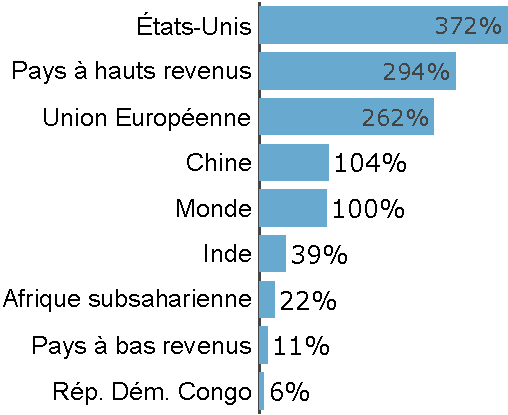
\includegraphics[width=.56\textwidth]{../figures/policies/GDP_pc_PPP_few_fr.pdf}}% https://data.worldbank.org/indicator/NY.GDP.PCAP.PP.CD?contextual=default&end=2021&locations=EU-ZG-XD-XM-1W-IN-US-CD-BI-LU-CN&start=2021&view=bar
\end{figure}

\section{Le lien entre climat et pauvreté} 

Quiconque se préoccupe du bien-être des humains souhaite mettre fin à la pauvreté. 
De même, il n'est pas nécessaire d'attacher une valeur intrinsèque à la Nature ou à la biodiversité pour vouloir lutter contre le changement climatique~; il suffit de se soucier du bien-être des humains. Le changement climatique met en péril les conditions de vie de larges catégories de population, non seulement dans les générations futures mais aussi chez nos contemporains, % mais aussi contemporaines
en particulier dans les pays tropicaux. En effet, le réchauffement est d'autant plus problématique dans les zones qui sont déjà chaudes --- et abritent l'essentiel des populations pauvres, car ces zones sont davantage exposées à la sécheresse, à la baisse des rendements agricoles, et à la difficulté à travailler en plein air (ou sans climatisation). Non seulement les plus pauvres subissent de plein fouet les effets du changement climatique, mais ils manquent de moyens pour y faire face~: %les populations qui ont à peine de quoi se nourrir
ils n'ont pas les ressources pour acheter un climatiseur, construire une digue ou migrer dans une zone épargnée. Non seulement la pauvreté accroît la vulnérabilité au changement climatique, mais le changement climatique augmente le risque de pauvreté. Ainsi, il est estimé qu'entre 32 et 132 millions de personnes basculeront dans l'extrême pauvreté dès 2030 à cause du changement climatique (notamment à travers ses effets sur la santé et les prix des denrées agricoles)\footnote{\cite{jafino_revised_2020}.}. En réduisant la croissance des pays les plus pauvres, le changement climatique augmente les inégalités~: il est estimé que l'écart de revenus entre les pays les plus riches et les plus pauvres s'est déjà accru de 25~\% sous l'effet du changement climatique\footnote{\cite{diffenbaugh_global_2019,khalfan_climate_2023}.}. %Aussi, dès l'an 2000, 166~000 morts étaient imputables annuellement au changement climatique, principalement à cause de ses conséquences en termes de malnutrition, diarrhée et malaria en Afrique et en Asie du Sud\footnote{\cite{patz_impact_2005}.}. 

% Tandis que les principales victimes du changement climatiques sont les générations futures et les populations déjà vulnérables, ce sont les populations les plus aisées qui sont à l'origine des émissions de gaz à effet de serre et ont bénéficié du confort permis par les énergies fossiles. L'enjeu du changement climatique est donc celui d'une injuste répartition des richesses. Pour schématiser, l'opulence d'occidentaux actuels et passés s'est faite au détriment de personnes vulnérables dans les pays du Sud et les générations futures. 

Le changement climatique soulève la question de la répartition mondiale et temporelle du pouvoir, de la richesse, et des opportunités. %et des capacités. 
En effet, la répartition des émissions de gaz à effet de serre est extrêmement inégale~: alors que les 1~\% d'États-uniens les plus riches émettent en moyenne 318~tCO$_\text{2}$e par an, l'Indien moyen en émet 2~t et les 10~\% les plus pauvres du Honduras ou du Mozambique n'en émettent que 0,1~t. %\footnote{\citet{chancel_carbon_2015}.}. 
Au niveau mondial, les 1~\% au sommet sont responsables de 50~\% de plus d'émissions que la moitié de l'humanité en bas de l'échelle (prise dans son ensemble)\footnote{\cite{chancel_carbon_2015,bruckner_impacts_2022}.}. 
Et contrairement à de nombreux Africains ou Sud-Asiatiques pauvres qui ne sont pas encore nés, les occidentaux riches et âgés à forte empreinte carbone ne souffriront probablement pas tellement du changement climatique et n'ont donc que peu intérêt à modifier leur mode de vie opulent, à moins qu'ils se soucient du bien-être de leurs descendants ou des humains en général\footnote{Comme le montrent les indices de vulnérabilité \citep{chen_university_2015} ou les estimations des dommages du changement climatique en fonction du PIB des pays \citep{burke_global_2015}.}. 
% Reconnaître que les intérêts financiers à court terme de l'élite vont à l'encontre du développement soutenable aide à comprendre que la solution ne viendra probablement pas des dirigeants actuels. 
Ainsi, pour prévenir les impacts dramatiques du changement climatique, il est trompeur de formuler la question simplement en termes de température, %problème environnemental, 
car le cœur du problème réside dans les inégalités entre les humains qui diffèrent en termes de richesse, de localisation ou de génération. En tant que telle, une solution au changement climatique ou à ses impacts ne peut être satisfaisante que si elle est équitable, et donc qu'elle implique un transfert substantiel de ressources des riches vers les pauvres et des générations présentes vers les générations futures.%d'aujourd'hui %(par exemple, par le biais de taxes sur le carbone) 
% vers les pauvres de demain.% (par exemple, par le biais de fonds d'adaptation). TODO: remettre l'ancienne formulation, pck on ne veut pas transmettre de la génération actuelle vers future si la future est plus riche
% BOF fait peur aux riches? préciser que ça peut se limiter aux très riches?
% TODO Peut-être qu'avant de dire ca il serait utile de résumer avec quelque chose comme ca : "Lutter contre le changement climatique c'est donc lutter contre les inégalités qu'il cause ou exacerbe, mais c'est aussi décider de la répartition des efforts dans cette lutte. Pour être satisfaisante, une solution au changement climatique...doit être équitable..."

% Une solution au problème couplé des inégalités et du changement climatique nécessitera un élargissement des perspectives. Qui cherche-t-on à favoriser le plus dans ses choix politiques ? Répondre à cette vaste question, en traçant une ligne entre "alliés" et "ennemis", permet de synthétiser l'orientation politique de chacun. On peut classer les gens sur une échelle allant du plus petit au plus grand groupe soutenu : soi-même, ses proches, son ethnie ou sa région, sa nation ou sa religion, tous les humains, l'ensemble de la biosphère. Dans la mesure où nous ne pouvons ressentir de l'empathie, nouer des liens et négocier une solidarité réciproque qu'avec ceux avec qui nous interagissons, il est compréhensible que les humains aient historiquement évolué en clans luttant les uns contre les autres pour le contrôle des ressources. Cependant, pour parvenir à une prospérité harmonieuse, nous devrions nous unir dans un groupe universel de solidarité et lutter ensemble contre des ennemis extérieurs (maladies, catastrophes climatiques) plutôt que contre des personnes avec lesquelles nous pourrions discuter et résoudre pacifiquement nos conflits. Grâce à Internet, il est désormais possible de tisser un réseau de liens interpersonnels nécessaires à la construction d'une société sûre et durable. De plus, l'instauration de la confiance entre les personnes est susceptible de produire des effets positifs importants sur la société, tels qu'une meilleure santé et une réduction des inégalités [Elgar2010] À une époque où les tendances nationalistes et égoïstes gagnent du terrain, il est donc crucial que les humains élargissent leur communauté de solidarité et pensent à long terme. Ce type de pragmatisme doit devenir dominant dans un avenir proche pour que l'opinion générale, les dirigeants et les institutions favorisent équitablement tous les humains (y compris les générations futures) au lieu de défendre les intérêts financiers à court terme de leurs proches ou de leur nation. Un tel humanisme est crucial pour le sort des personnes faibles et du climat. De plus, comprendre que tous les destins sont interdépendants et que le bonheur de chacun dépend des perspectives de bien-être accordées à quiconque[pickett_income_2015] est la seule spiritualité dont la diffusion peut permettre un bonheur durable au plus grand nombre, en projetant un avenir désirable (au lieu de prédire un avenir déprimant). Pour ces raisons, la solution au changement climatique réside davantage dans la bataille d'idées entre humanistes et individualistes que dans le marchandage diplomatique entre pays. 

\chapter{La nécessité de redistribution mondiale\label{ch:redistribution_necessaire}}

\section{Une prescription morale}
Qu'elle soit religieuse, philosophique ou intuitive, la morale prescrit généralement des transferts des personnes à hauts revenus vers les personnes à bas revenus, et donc des pays à hauts revenus vers les pays à bas revenus. C'est le cas de l'utilitarisme, la théorie éthique de référence utilisée en économie. L'utilitarisme attribue le même poids à chaque personne et justifie ainsi le transfert d'un euro d'une personne riche à une personne pauvre, puisqu'un euro procurera plus de satisfaction à cette dernière. D'après la théorie de la taxation optimale, ce raisonnement est valable tant qu'une augmentation des prélèvements n'incite pas les plus riches à réduire, expatrier ou dissimuler leur activité au point de diminuer les recettes obtenues. Des économistes ont calculé le système fiscal optimal en tenant compte de ces effets. Celui-ci réduirait drastiquement les inégalités entre pays et procurerait un revenu minimum de 250~\$ par mois au niveau mondial\footnote{Dans ces calculs, \citet{kopczuk_limitations_2005} se limitent à un taux unique (une \textit{flat tax}) et ne s'autorisent pas un barème progressif. Sans cette restriction, le véritable optimum serait encore plus redistributif.}. La théorie de la taxation optimale ne peut rationaliser la situation actuelle qu'en tordant le cou à la morale. En effet, des chercheurs ont montré que la quasi-absence de transferts internationaux n'est optimale que si on attribue un poids 2~000 fois plus élevé à un États-unien qu'à un Congolais (ou bien, si on attribue une valeur 100 fois supérieure à l'États-unien et qu'on considère que seul un vingtième de l'argent transféré arrivera à son destinataire, le reste étant détourné par la corruption). %de distordre les poids de sorte que la satisfaction d'un États-unien vaille autant que celle de 2~000 Malgaches. 

\section{Un engagement juridico-diplomatique}
Au-delà des considérations éthiques, l'impératif de redistribution mondiale a des fondements juridiques. En 2015, l'ensemble des pays a adopté les Objectifs de développement durable (ODD), au premier rang desquels se trouve l'élimination de l'extrême pauvreté d'ici à 2030. Or, les pays à bas revenus n'ont pas les ressources domestiques suffisantes pour éliminer l'extrême pauvreté. En effet,  dans les 19 pays les plus pauvres, exproprier tous les revenus à partir de 13~\textit{\$} par jour ne suffirait pas à financer des transferts suffisants pour faire passer leurs 700 millions d'habitants au-dessus de 2~\textit{\$} par jour d'ici à 2030. Même en faisant l'hypothèse très optimiste d'une croissance du revenu moyen de 7~\% par an d'ici à 2030% (soit le maximum observé dans le monde dans les cinq années qui ont précédé la Covid)
, exproprier tous les revenus au-delà de 7~\textit{\$} par jour ne suffirait pas à éliminer l'extrême pauvreté dans un pays tel que Madagascar\footnote{Ces calculs sont inspirés de \citet{bolch_arithmetics_2022}, reposent sur les données \textit{Poverty and Inequality Platform} de la Banque mondiale, et sont reproductibles sur \href{https://github.com/bixiou/domestic\_poverty\_eradication/code\_poverty/main.R}{github.com/bixiou/domestic\_poverty\_eradication}.}. En d'autres termes, il est impossible d'atteindre le premier ODD sans transferts internationaux. Et ce, alors que le premier ODD se borne à assurer un revenu à peine suffisant pour ne plus avoir faim. Le transfert nécessaire pour ce premier ODD correspond à 0,1~\% du PIB mondial, soit autant que les dépenses de nourriture pour les animaux de compagnie\footnote{Cf. \href{https://www.grandviewresearch.com/industry-analysis/pet-food-industry}{grandviewresearch.com}.}. % 2019 poverty gap = 2.6% of $2.15 / world GDP of 16865 https://data.worldbank.org/indicator/SI.POV.GAPS; https://www.grandviewresearch.com/industry-analysis/pet-food-industry

Pour s'assurer une vie décente, qui garantit l'accès à l'eau, l'assainissement, l'éducation, à un système de santé, à une capacité minimale à se déplacer et socialiser, on estime qu'il faut un revenu d'au moins 7,5~\textit{\$} par jour\footnote{Cf. Chapitre \ref{ch:premier_pas}.}. 
600 millions de personnes vivent dans un pays où le PIB par habitant est inférieur à ce seuil, et où il est donc rigoureusement impossible d'assurer une vie décente à chacun en mobilisant les seules ressources domestiques. 
Au total, près de la moitié des humains vit sous ce seuil de pauvreté\footnote{Cf. \href{https://ourworldindata.org/grapher/distribution-of-population-between-different-poverty-thresholds-up-to-30-dollars}{ourworldindata.org}.}. Combler l'écart qui les sépare de ce seuil coûterait 2~\% du PIB mondial en 2030\footnote{En parité de pouvoir d'achat, cet écart (le \textit{poverty gap}, qu'on peut traduire par \textit{l'étendue de la pauvreté}) est de 5~800 milliards de dollars, soit 4~\% du PIB mondial de 140~000 milliards. Si on tient compte de la croissance et des écarts de niveaux des prix entre pays, on trouve %une estimation basse à 
2~\% du PIB mondial en 2030.}. % https://data.worldbank.org/indicator/SI.POV.UMIC.GP https://data.worldbank.org/indicator/NY.GDP.MKTP.PP.KD
% PG 7,5 growth: none = 5.8T$PPP ~ 3T$ in nominal, i.e. 3%. With optimistic growth, it is 2.7T$, i.e. more than twice less. To convert PPP into nominal: https://data.worldbank.org/indicator/NY.GDP.PCAP.PP.KD?locations=ZG-8S&year_high_desc=true https://data.worldbank.org/indicator/NY.GDP.PCAP.KD?locations=ZG-8S&year_high_desc=true

En 1970, les pays industrialisés ont pris l'engagement d'allouer 0,7~\% de leur PIB à l'aide publique au développement, dont 0,2~\% du PIB pour les pays les moins avancés. Cet engagement, renouvelé en 2005 et 2015, n'a été jamais été tenu\footnote{Plus précisément, l'aide effective s'élève à seulement la moitié de l'aide promise, dont seulement 0,06~\% pour les pays les moins avancés et seule une poignée de pays respectent leur engagement : le Luxembourg, la Suède, la Norvège, l'Allemagne et le Danemark 
\citep{oecd_oda_2023}.}. 
On estime que l'essentiel des ODD pourraient être atteints si les pays industrialisés respectaient enfin cet engagement\footnote{\citet{sdsn_sdg_2019}.}. Pour atteindre une version maximaliste des ODD (y compris assurer l'accès à une énergie propre) ou un autre objectif ambitieux au regard du statu quo (tel qu'assurer 7,5~\textit{\$} par jour à chacun), les pays à hauts revenus devraient transférer davantage de ressources, probablement entre 2 et 5~\% 
de leur PIB. % PIB high-income/all: 61% (nominal https://data.worldbank.org/indicator/NY.GDP.MKTP.CD?end=2022&locations=XD-1W&start=2022&view=bar) / 46% (PPP https://data.worldbank.org/indicator/NY.GDP.MKTP.PP.KD?end=2022&locations=XD-1W&start=2022&view=bar)
% Il va sans dire que pour développer des services de santé, d'éducation, une énergie décarbonée, et plus généralement atteindre l'ensemble des ODD, la solidarité internationale est indispensable. Pour assurer 
% Plus généralement, 12 ODD sur les 17 concernent la pauvreté, les inégalités et le changement climatique. Si les pays à bas revenus n'ont déjà pas les ressources nécessaires pour éliminer l'extrême pauvreté (estimées à 0,1\% du PIB mondial), % 2019 poverty gap = 2.6% of $2.15 / world GDP of 16865 https://data.worldbank.org/indicator/SI.POV.GAPS
% il va sans dire qu'une redistribution internationale est nécessaire pour développer des services de santé, d'éducation, une énergie décarbonée, et plus généralement atteindre l'ensemble des ODD.

% De tels transferts seraient colossaux. Mais ils pourraient être intégralement supportés par les millionnaires. En se limitant au millième d'humains les plus riches, qui ont une fortune supérieure à 5 millions d'euros, et en ne taxant que leur fortune au-delà de ce seuil, avec un taux effectif progressant de 1\% pour une fortune de 10 millions d'euros à 10\% pour une fortune de 100 milliards, on récolterait environ 2~\% du PIB mondial, et leur fortune ne baisserait même pas (puisque la plupart des milliardaires ont des rendements supérieurs à 10\%). 
% À l'aide d'une taxation plus progressive, qui démarrerait à 500~000 euros, avec un taux de 0,25~\% pour une fortune d'un million d'euro (soit une taxe de 2~500\euro{} par an), et progressant jusqu'à un taux de 20\% sur les plus grosses fortunes, les recettes pourraient atteindre 6\% du PIB mondial. Si une telle redistribution était mise en place, les classes moyennes seraient largement épargnées. Certes, des emplois seraient détruits dans le secteur du luxe, puisque les plus fortunés consommeraient un peu moins, mais d'autres secteurs seraient portés par le développement des pays du Sud et créeraient des emplois orientés vers la production de biens exportés, notamment dans l'industrie. 

% Si les pays de l'OCDE tenaient leur promesse d'allouer 0,7~\% de leur PIB à l'aide publique au développement, dont 0,2~\% du PIB pour les pays les moins avancés, les ODD pourraient être remplis\footnote{Cf. \citet{sdsn_sdg_2019}.}. 
% Flux dans l'autre sens

\section{Un impératif pour la décarbonation du Sud}
Enfin, les transferts internationaux sont une condition \textit{sine qua non} pour que les pays à bas revenus se décarbonent. D'une part, ces pays font face à d'autres priorités que la décarbonation et déploient donc le système énergétique le plus abordable --- reposant souvent sur le charbon. D'autre part, ces pays font valoir --- à juste titre --- qu'ils sont les plus vulnérables au changement climatique et qu'ils n'y ont contribué que marginalement\footnote{L'Afrique et l'Asie du Sud sont responsables de 6~\% des émissions de CO$_\text{2}$ cumulées. % https://ourworldindata.org/contributed-most-global-co2
}. Dans les négociations internationales, ces pays annoncent généralement deux objectifs de réductions d'émissions : un objectif inconditionnel peu ambitieux et un objectif ambitieux conditionné à des financements extérieurs. Par exemple, l'Éthiopie s'est engagée à réduire inconditionnellement ses émissions de 14~\% en 2030 par rapport à un scénario sans action climatique, et conditionne une réduction de 69~\% à un financement de 250 milliards de dollars. %\footnote{Cf. \href{https://www.climatewatchdata.org/custom-compare/overview?section=fairness\_and\_ambition&targets=NGA-revised\_first\_ndc%2CETH-revised\_first\_ndc%2CIDN-}{climatewatchdata.org}.}. % https://www.climatewatchdata.org/custom-compare/overview?section=fairness_and_ambition&targets=NGA-revised_first_ndc%2CETH-revised_first_ndc%2CIDN-
% En NPV, l'Éthiopie recevrait 1.3T$ dans le Plan, et le pays recevrait 258G$ sur la période 2030-33.
Parallèlement, les pays en développement (appuyés par le Secrétariat général de l'ONU) appellent à des transferts de 100 milliards de dollars annuels pour compenser les pertes et dommages climatiques dus aux émissions des pays développés\footnote{Cf. \cite{tc_proposal_2023,sgnu_bridgetown_2023}.}. Si les experts estiment que les transferts requis seraient deux à quatre fois supérieurs à ce montant, seuls 700 millions ont été \textit{promis} en 2023 lors de la COP 28% (soit à peine autant que les revenus des cinq joueurs de foot les plus riches)
\footnote{Cf. \cite{songwe_climate_2023,markandya_integrated_2019,robinson_valuing_2021} et \href{https://www.theguardian.com/environment/2023/dec/06/700m-pledged-to-loss-and-damage-fund-cop28-covers-less-than-02-percent-needed}{www.theguardian.com/environment/2023/dec/06/700m-pledged-to-loss-and-damage-fund-cop28-covers-less-than-02-percent-needed}% et \href{https://frontofficesports.com/the-10-highest-paid-soccer-players-in-the-world-for-2023/}{frontofficesports.com/the-10-highest-paid-soccer-players-in-the-world-for-2023}
.}.

Plus généralement, l'arène internationale tend à se polariser entre le Sud, qui exige un ordre mondial plus juste, et le Nord, qui rechigne à abandonner sa position dominante. Ainsi, l'Union africaine a récemment appelé à un régime mondial de tarification du carbone, à une taxe sur les transactions financières et à une réforme du système financier, afin de bénéficier de financements dédiés, abordables et pérennes pour le climat, dissociés des intérêts nationaux et géopolitiques\footnote{\cite{african_union_african_2023}.}. Les pays du Sud critiquent également les négociations internationales sur la taxation des sociétés, qui ont lieu sous l'égide de l'OCDE et excluent de nombreux pays à bas revenus. En novembre 2023, bien que les pays de l'OCDE aient voté contre, les pays du Sud ont fait adopter une résolution à l'ONU qui établit une Convention sur la taxation (à la manière des COP sur le climat). Les pays du Sud espèrent que ce cadre de négociations sera plus favorable à leurs intérêts que l'OCDE. Or, il y a un espoir que les pays du Nord accèdent à certaines demandes du Sud. 
% Dans un monde qui verse de plus en plus dans le nationalisme et l'autoritarisme, 
Que ce soit pour défendre des valeurs humanistes ou redorer son image bien souvent entachée, 
l'Occident cherche à s'afficher comme un modèle fondé sur les droits humains et la démocratie. 
Ainsi, Ursula von der Leyen, la présidente de la Commission européenne, a récemment pris parti pour la tarification mondiale du carbone\footnote{Cf. son \href{https://twitter.com/vonderleyen/status/1700416700238225659}{Tweet} du 9 septembre 2023.}, et un groupe de travail sur la taxation internationale (notamment du carbone) a été lancé en décembre 2023 conjointement par la France, le Kenya, l'Espagne et la Barbade\footnote{Cf. \href{https://www.elysee.fr/admin/upload/default/0001/15/91b013291db03bcc5f2f6b84de39a81ae0c04c7d.pdf}{https://bit.ly/taskforce\_tax}.}. 
Les valeurs humanistes seraient enfin correctement défendues en cas d'un accord international pour le climat etd' une taxation juste qui mettrait à contribution les pays du Nord. Un tel accord aurait le potentiel de refonder la géopolitique sur des bases saines et de pacifier les relations internationales. A contrario, il a été montré que le changement climatique accroît le risque de conflits armés, notamment en Afrique\footnote{\cite{burke_warming_2009,eberle_heat_2020}.}.

Dans les prochains chapitres, nous proposons un Plan mondial pour mettre fin au changement climatique et à l'extrême pauvreté, impliquant d'importants transferts Nord--Sud, tout en étant accepté par %able pour 
les populations des pays du Nord.
% ODA for LDCs: only Luxembourg is above the objective of 0.2% of GNI (SDG 17.2) https://data.worldbank.org/indicator/DC.ODA.TLDC.GN.ZS?locations=US-GR-LU-SE-GB&most_recent_value_desc=true
% 19 pays (570M en 2022, 700M en 2030) ne pourraient pas éradiquer l'extrême pauvreté même en expropriant tous les revenus au-delà de 13$/jour. Pays comme la RDC ne pourrait pas mettre fin à l'extrême pauvreté en 2030, même avec une croissance de 6% et en expropriant tous les revenus au-delà de 7$/jour.

% Addressing global poverty, inequalities and climate change are at the heart of the universally agreed Sustainable Development Goals (SDG). % 12 out of  17
% It has been pointed out that low-income countries generally do not have enough domestic resources to eliminate the poverty gap in the short run.\cite{bolch_arithmetics_2022} % In other words, it would hardly be possible to achieve the first SDG and end extreme poverty by 2030 without international transfers. => Careful, Bolch use a poverty line above the SDG one.



\chapter{Le cœur du Plan mondial pour le climat\label{ch:coeur}}
% Le plan mondial pour le climat : les grands principes (description de la mesure, des trajectoires)

% \section{Le cœur du Plan}

On a vu au Chapitre \ref{ch:statu_quo} que l'humanité disposait d'un budget carbone à ne pas dépasser pour maintenir le réchauffement sous une cible donnée. L'accord de Paris établit cette cible. Cet accord, signé par l'intégralité des pays en 2015,  vise à contenir le réchauffement <<~nettement en dessous de 2\textdegree{}C (...) en poursuivant l'action menée pour limiter l'élévation de température à 1,5\textdegree{}C~>>. \\

Comment garantir une trajectoire d'émissions conforme à ce budget carbone~? 

Le plus sûr serait de plafonner les émissions mondiales, grâce à un plafond annuel qui décroît en conformité avec l'objectif. \\

Comment alors allouer les émissions de CO$_\text{2}$ permises~? 

Le plus simple % naturel, élémentaire
est d'allouer un même permis d'émissions à chaque humain. \\

Faut-il autoriser la revente des permis d'émissions~? 

Oui, % Passer en FAQ la suite ?
instaurer un marché du carbone est préférable à un système de quota carbone non échangeable pour plusieurs raisons, détaillées dans la Foire Aux Questions (FAQ, p. \pageref{q:rationnement}).\\ % La FAQ contient également des justifications détaillées de ce système comparé à d'autres, explique en quoi il est favorable aux plus modestes et obligerait les riches à réduire leurs émissions.% défavorable aux plus riches. %(Chapitre \ref{ch:faq}). 

Ces trois réponses suffisent à saisir l'essentiel du Plan mondial pour le climat.

\paragraph{Prévenir certains malentendus}
Il est important de comprendre qu'en instaurant un plafonnement des émissions, les émissions mondiales sont par construction égales à ce plafond, grâce à des mécanismes (détaillés aux Sections \ref{sec:pcp_quota} et \ref{sec:implementation}) qui empêchent son dépassement. C'est le principal intérêt de ce Plan.

% Ce qui lève mon objection d'une affirmation sans preuve et permet de laisser éventuellement la suite sur la pauvreté en place, même si l’enchaînement me paraîtrait plus naturel si votre critique de la compensation carbone suivait directement.
% BOF prix du carbone => coût du carbone? (pck le prix est plus faible que le coût s'il y a d'autres mesures, et le marché fixe un prix, pas un coût)
% BOF enlever?
Ce plafonnement règle la question de la température, %trajectoire climatique, 
mais pas la question sociale~: c'est la répartition des permis d'émissions qui détermine comment les efforts sont partagés. La répartition égalitaire que nous proposons permet d'opérer une importante redistribution Nord--Sud et de mettre fin à l'extrême pauvreté. 

Pour éviter une confusion fréquente, notons d'emblée que ce système \textit{ne} permettrait \textit{pas} d'acheter des crédits de compensation carbone grâce à des projets de reforestation. Le système proposé ressemble au marché du carbone européen en place depuis 2005, mais est radicalement différent du marché --- dysfonctionnel et propice au greenwashing --- de la compensation carbone\footnote{Le marché européen plafonne les émissions des secteurs de l'industrie et de l'électricité, selon une trajectoire qui décroît jusqu'à zéro en 2040. Il va être complété en 2027 par un deuxième marché du carbone qui couvrira les émissions des transports et des bâtiments. Il ne faut pas confondre ces marchés du carbone avec le marché de la \textit{compensation} carbone, qui permet à des entreprises ou à des individus volontaires d'acheter des crédits carbone pour <<~compenser~>> leurs émissions grâce à des projets (de type reforestation) dans des pays en développement. La compensation carbone pose problème car elle ne garantit pas une réduction des émissions mondiales. En effet, il n'est pas clair que les projets financés entraînent une réduction d'émissions \textit{permanente} (par exemple, une zone reforestée lors du projet peut être déforestée plus tard) et \textit{additionnelle} (par exemple, une forêt aurait pu repousser même en l'absence de financement, ou bien la reforestation à un endroit peut générer une \textit{fuite de carbone} en provoquant une déforestation à un autre endroit). Pour ces raisons, les crédits carbone ne sont pas éligibles sur les marchés européens du carbone. Ces derniers réduisent véritablement les émissions européennes.}.
%Déjà, si les permis d'émissions ne sont pas échangeables, cela signifie soit que des centaines millions de personnes (notamment dans les pays du Nord) devraient diviser leurs émissions par deux ou trois du jour au lendemain (les mettant dans l'impossibilité de poursuivre leurs activités), soit qu'on allouerait (dans un premier temps) davantage de permis d'émissions aux personnes qui polluent davantage (ce qui romprait avec le principe d'égalité cher aux défenseurs des quotas non échangeables). A contrario, si les permis sont échangeables, les pollueurs auraient une certaine latitude pour choisir leurs émissions et du temps pour adapter progressivement leurs activités et changer leur équipement, tandis que les personnes avec une faible empreinte carbone pourraient revendre leurs permis d'émissions inutilisés et ainsi gagner du pouvoir d'achat. Ainsi, tant les pollueurs que les frugaux bénéficieraient de la flexibilité permise par le marché. D'ailleurs, le bénéfice potentiel serait tellement important que l'émergence d'un marché noir serait difficile à empêcher dans le cas d'un système de quotas non échangeables. Vous vous dites peut-être qu'un marché du carbone serait immoral ou injuste, car il permettrait aux plus riches de continuer à polluer. Pourtant, un tel système opérerait une redistribution des pollueurs vers les frugaux : ceux-là devant payer pour acheter des permis d'émissions à ceux-ci. En outre, mettre en place un marché du carbone n'empêche pas d'interdire par ailleurs les consommations jugées superflues, telles que les yachts, les jets privés, voire les SUV. Enfin, si on considère injuste que les plus riches soient capables de préserver un mode de vie dispendieux dans un tel système, n'est-ce pas parce qu'on considère l'extrême richesse comme injuste~? Si c'est le cas, autant s'attaquer à la fortune directement, plutôt que de passer par des moyens détournés. En effet, plafonner les émissions de Rupert Murdoch ne l'empêcherait pas d'utiliser son empire médiatique pour minimiser, voire nier le changement climatique. %d'Elon Musk ne l'empêcherait pas d'acheter Twitter et d'en contrôler l'algorithme. 

% Un dernier argument contre le marché est qu'il permettrait des enrichissements illégitimes à cause de la fraude ou la spéculation. 

% Le système esquissé ci-dessus semble réguler les \textit{individus}. J'ai fait comme si % BOF c'était pas clair que j'avais fait comme si, on peut virer ce passage
% les individus auraient la responsabilité d'acheter ou vendre des permis d'émissions, alors qu'on n'a même pas les données pour mesurer précisément les émissions de quelqu'un. En réalité, on peut obtenir des effets équivalents au système esquissé précédemment avec un fonctionnement bien plus simple, qui régule les \textit{entreprises}~: 

\paragraph{Fonctionnement}
Le système esquissé ci-dessus peut être mis en œuvre de la façon suivante. Chaque année, un nombre limité de permis d'émissions est créé, en conformité avec la trajectoire d'émissions qu'on s'est fixée. Ces permis d'émissions sont mis aux enchères auprès des entreprises à la source des émissions de CO$_\text{2}$, et en particulier celles qui mettent sur le marché % PNON extraient ?
du charbon, du pétrole ou du gaz. Ces entreprises doivent se procurer des permis correspondant à leurs émissions. Enfin, les recettes générées par la vente de permis sont redistribuées en un revenu de base égal pour tous les humains. 

\paragraph{Qui paie~? Qui reçoit~?}
Le revenu de base est égal aux recettes générées divisées par la population. Or, les recettes générées sont égales au prix du carbone multiplié par les émissions mondiales de carbone. Ainsi, le revenu de base est égal au prix du carbone multiplié par l'empreinte carbone moyenne d'un humain. 

Bien que, pour des considérations pratiques, on distribuerait aux individus de l'argent plutôt que des permis d'émission, ces deux options sont équivalentes. En effet, imaginons que chaque humain reçoive le même permis d'émission et puisse le revendre aux entreprises polluantes sur le marché du carbone. La somme qu'il en tirerait serait égale au prix du carbone multiplié par le quota individuel, c'est-à-dire exactement le revenu de base. Ainsi, il y a une correspondance parfaite entre allocation égalitaire des permis d'émissions ou allocation égalitaire des recettes. % PNON égal droit à polluer ?

% Même si, en apprence, le prix du carbone est payé par les entreprises polluantes, il faut bien comprendre qu'au bout du compte ce sont les consommateurs qui paient ce coût. % PNON => je ne dis pas que l'apparence est fausse dans ma formulation, qui est plus nuancée
Même s'il serait avantageux % accommodant
d'affirmer que le prix du carbone est payé par les entreprises polluantes, il est plus juste d'expliquer que ce sont les consommateurs qui en supportent le coût. 
En effet, les entreprises polluantes répercutent le coût des permis d'émissions en hausses de prix, si bien que chaque individu fait face à une hausse de dépenses, égale au prix du carbone multiplié par son empreinte carbone. De ce fait, le revenu de base couvre tout juste le prix du carbone payé pour un individu dont l'empreinte carbone est égale à la moyenne mondiale. Les personnes ayant une empreinte carbone plus élevée que la moyenne mondiale perdent en pouvoir d'achat\footnote{Ce résultat découle d'hypothèses justifiées en Annexe \ref{app:indiv}. L'empreinte carbone et sa moyenne mondiale mentionnées sont celles \textit{après} l'entrée en vigueur du Plan.
%qui ne tient compte ni de la diminution de l'empreinte carbone induite par le prix du carbone, ni de la hausse du pouvoir d'achat induite par le revenu de base. La hausse de dépenses sera en réalité inférieure à cette approximation pour un individu dont l'empreinte carbone diminue suite à la mesure, ce qui sera le cas pour l'individu moyen. Le revenu de base sera lui aussi plus faible, puisqu'il sera égal au prix du carbone multiplié par l'empreinte carbone moyenne \textit{après} la réforme. % PNON put back?
}. À l'inverse, les personnes avec une faible empreinte carbone y gagnent. En d'autres termes, le système proposé opère une redistribution mondiale des pollueurs vers les frugaux --- donc, en première approximation, des riches vers les pauvres. 

Pour en savoir plus, la FAQ (p. \pageref{q:riches}) contient des justifications de ce système comparé à d'autres, explique en quoi il est favorable aux plus modestes et obligerait les riches à réduire leurs émissions.

% D'un point de vue théorique, ce système \textit{corporatif} est équivalent au système individuel précédent. En effet, dans le système corporatif, les entreprises polluantes répercutent le coût des permis d'émissions en hausse de prix, si bien que chaque individu ($i$) fait face à une hausse de dépenses ($\Delta d_i$) égale au prix du carbone ($p$) multiplié par son empreinte carbone ($e_i$)~: % PNON remettre formule
% $$ \text{hausse de dépenses}_i = \Delta d_i = p \times e_i\text{.}$$
% Quant aux recettes générées, elles correspondent au produit du prix du carbone par l'ensemble des émissions, de sorte que le revenu de base ($r$) est égal au prix du carbone multiplié par l'empreinte carbone moyenne ($\overline{e} = \frac{1}{N} \sum_{i=1}^N e_i$)~:  
% $$ \text{revenu de base} = r = p \times \overline{e}\text{.}$$
% Dans le système individuel, les permis d'émissions sont alloués de façon égalitaire aux individus, donc les permis d'émissions d'un individu correspondent à l'empreinte carbone moyenne ($\overline{e}$). Ainsi, si une personne revendait tous ses permis d'émissions (au prix $p$), elle toucherait un montant équivalent au revenu de base. Par ailleurs, cet individu devrait alors acheter des permis pour couvrir ses émissions, pour un montant égal au prix du carbone multiplié par son empreinte ($p \times e_i$). Dans les deux cas, on retombe sur le même calcul. Le gain net pour un individu est égal à~: 
% $$\text{gain net}_i = r - \Delta d_i = p \times \left( \overline{e} - e_i \right)\text{.}$$
% Le système reposant sur les individus est intéressant d'un point de vue théorique, puisqu'il permet de montrer l'équivalence entre allocation des permis d'émissions et allocation des recettes d'une tarification carbone. En revanche, le système d'enchères aux entreprises est le seul qui soit réaliste à administrer. 

\paragraph{Taxe ou quota~?}
Pour conclure, notons que ce système fixe une quantité~: le régulateur fixe un quota d'émissions et laisse le marché déterminer le prix du carbone. À l'inverse, on pourrait imaginer une taxe carbone~: le régulateur fixe le prix et laisse le marché déterminer les émissions. Pour peu que le prix du carbone soit le même dans le système qui fixe la quantité et celui qui fixe le prix, les deux systèmes sont strictement équivalents (ils entraînent les mêmes émissions tarifées au même prix). Notre proposition repose sur un système qui fixe la quantité puisque l'objectif premier est de respecter le budget carbone (or, fixer le prix ne permet pas de prévoir précisément les émissions). Certes, le système proposé ne permet pas de prévoir précisément le prix du carbone, et un prix trop élevé serait problématique (car il entraînerait des coûts trop importants pour ajuster nos modes de vie). Mais le prix du carbone peut être réduit grâce à des mesures complémentaires (cf. Chapitre \ref{ch:premier_pas}), et il semble préférable de ne pas sacrifier l'ambition climatique. Cependant, on pourrait fixer le prix sans sacrifier l'ambition, à l'aide d'une taxe carbone dont le montant serait révisé annuellement de sorte à s'assurer que la trajectoire d'émissions soit conforme au budget carbone. Une telle taxe (dont on ne connaît pas précisément le montant plusieurs années à l'avance) serait in fine équivalente au quota que nous proposons. Ainsi, elle constituerait une variante tout à fait valable au Plan proposé, que je soutiendrais tout autant, la différence entre les deux relevant du détail. 

\paragraph{Conclusion}
Pour résumer, on peut mettre fin au réchauffement climatique en plafonnant les émissions et éliminer l'extrême pauvreté à l'aide d'un revenu de base. Un système simple et efficace pour traiter ces deux problèmes est de combiner ces deux solutions. Voici le cœur du Plan mondial pour le climat, % PNON changer cette fin?
qui constitue les deux premiers principes détaillés au Chapitre \ref{ch:principes}. Pour des considérations de justice et de géopolitique, quelques ajustements sont nécessaires pour compléter notre proposition~: je les décris aussi au Chapitre \ref{ch:principes}. %aux principes 3 et 4. 
Enfin, ce Plan mondial pour le climat doit être complémenté par d'autres mesures%, par exemple pour éviter que les classes moyennes des pays à hauts revenus ne soient perdantes
~: je les esquisse au Chapitre \ref{ch:premier_pas}.


\chapter*{\textit{Une journée à l'hôpital de Poitiers}}\label{ch:narr_poitiers}
\addcontentsline{toc}{chapter}{\nameref{ch:narr_poitiers}} 

Catherine est infirmière au CHU de Poitiers. Aujourd'hui, elle a préparé des gâteaux pour fêter la fin des travaux avec ses collègues~: maintenant que l'hôpital est rénové, finis les bruits de perceuse et surtout, finies les températures invivables en période estivale. Catherine, elle, n'a pas attendu que le Plan mondial fasse augmenter le prix du gaz %augmente (sous l'effet du Plan mondial) 
pour faire des travaux dans sa maison. Lorsqu'elle en a héritée en 2028, l'audit énergétique avait révélé qu'étant donné la hausse de prix anticipée, l'option la plus économe pour le chauffage consistait à isoler les murs et les combles, et remplacer la chaudière au fioul par une pompe à chaleur. Le remboursement des travaux coûte à Catherine un peu moins que ce qu'elle aurait dépensé en fioul, et lorsqu'elle aura fini de rembourser son crédit en 2041, elle gagnera vraiment au change. 

Dans son hameau cossu de Charassé, quasiment tout le monde a une voiture électrique. Catherine, elle, a opté pour un scooter électrique lorsqu'elle s'est débarrassée de sa vieille Twingo. Elle a fait ce choix pour pouvoir financer l'école de commerce de sa fille~: se passer de voiture, ça permet de sacrées économies, surtout avec la hausse du prix de l'essence. Et puis les embouteillages ne lui manquent pas. Même si elle appréhendait de ne plus faire ses courses en voiture, elle aime bien se faire livrer, finalement. En fait, le plus gênant, c'est pour partir en vacances avec son petit dernier. Alors qu'avant elle en avait pour deux heures de route pour aller chez ses parents aux Sables-d'Olonne, ça lui prend désormais six heures porte à porte~: un bus puis trois trains. Enfin ça, c'est quand elle ne trouve pas de covoiturage. Grâce à l'alerte qu'elle s'est paramétrée, elle réussit quand même à se faire des week-ends chez ses parents aussi régulièrement qu'avant. Elle saute sur l'occasion quand un conducteur fait un aller-retour similaire au sien, et fait parfois des belles rencontres. La dernière fois, elle a eu le béguin pour son conducteur~: un ancien ouvrier de l'usine de moteurs d'avion qui a fermé, reconverti dans la pose de panneaux solaires. En repensant à son sourire d'ange et son beau teint hâlé, Catherine espère vraiment retomber sur lui au prochain trajet.


\chapter{Un Plan largement soutenu\label{ch:soutien}}
% BOF scinder en deux chapitres et réorganiser?

% Un plan largement soutenu (soutien majoritaire dans 20 pays, avantage électoral aux partis de gauche qui l'incluraient dans leur programme, consensus en faveur de la répartition égalitaire de l'effort de décarbonation)
Outre ce livre et une vidéo YouTube\footnote{La vidéo résumant le livre en 30 minutes est disponible sur \href{https://bit.ly/CH_GCP}{bit.ly/CH\_GCP}.}, d'autres bénévoles et moi-même défendons le Plan mondial pour le climat auprès de multiples acteurs à travers l'association de plaidoyer que nous avons fondée, \textit{Global Redistribution Advocates}. % Je parle de GRA ici au cas où les gens referment le livre juste après
Notre motivation à défendre ce Plan découle du résultat de ma recherche académique. Depuis ma thèse, je me suis spécialisé dans les enquêtes d'opinion relatives au climat et à la redistribution. Ainsi, j'ai mené une enquête internationale dans 20 pays sur les attitudes envers les politiques climatiques, et une enquête complémentaire aux États-Unis et en Europe sur les opinions envers la redistribution mondiale des richesses. Bien que l'idée au cœur du Plan mondial pour le climat --- un quota carbone mondial avec une redistribution égalitaire des recettes --- soit ancienne et considérée comme la politique climatique canonique par les économistes, aucune enquête n'avait testé cette proposition auprès de l'opinion publique. Or, les enquêtes révèlent un soutien majoritaire à travers le monde. En outre, différentes méthodes d'enquêtes indiquent que le soutien est sincère et pourrait se matérialiser électoralement. 
C'est cet élément nouveau --- savoir que la population soutient un tel Plan, même dans les pays qui seraient perdants financièrement --- qui justifie de remettre cette idée sur la table des négociations internationales, et qu'on l'étudie sérieusement. Dans ce chapitre, je décrirai l'histoire de cette idée puis les résultats des enquêtes d'opinion.

% Outre l'écriture de ce livre, je défends le Plan mondial pour le climat à travers l'association de plaidoyer que j'ai fondée, \textit{Global Redistribution Advocates}. La motivation à défendre ce Plan découle du résultat de ma recherche académique. Depuis ma thèse, je me suis spécialisé dans les enquêtes d'opinion relatives au climat et à la redistribution. Ainsi, j'ai mené une enquête internationale dans 20 pays sur les attitudes envers les politiques climatiques, et une enquête complémentaire aux États-Unis et en Europe sur les opinions envers la redistribution mondiale des richesses. Bien que l'idée au cœur du Plan mondial pour le climat --- un quota carbone mondial avec une redistribution égalitaire des recettes --- soit ancienne et considérée comme la politique climatique canonique par les économistes, aucune enquête n'avait testé cette proposition auprès de l'opinion publique. Or, les enquêtes révèlent un soutien majoritaire et sincère à travers le monde. C'est cet élément nouveau --- savoir que la population soutient un tel Plan, même dans les pays qui seraient perdants financièrement --- qui justifie de remettre cette idée sur la table des négociations internationales, et qu'on l'étudie sérieusement. Dans ce chapitre, je décrirai l'histoire de cette idée puis les résultats des enquêtes d'opinion.

\section{Une vieille idée} 

\subsubsection{La genèse de l'idée}
Le principe du pollueur-payeur est une idée de base en économie, qui remonte à \citet{pigou_economics_1920}. Le principe consiste à faire payer les coûts externes (en l'occurrence, les dégâts causés par le changement climatique) à la personne qui les engendre (ici, l'émetteur de gaz à effet de serre). Cette tarification peut prendre aussi bien la forme d'un marché de quotas que d'une taxe. Le coût qu'elle entraîne pour le pollueur l'encourage à réduire son activité ou à la rendre moins polluante, ces alternatives étant désormais comparativement moins coûteuses. %le coût de ces alternatives étant désormais relativement avantageux. 
% Pour neutraliser les coûts externes résiduels, les recettes engendrées devraient servir à prévenir ou remédier aux préjudices causés. 
Pour compenser les préjudices causés par la pollution restante, les recettes engendrées par la tarification de celle-ci devraient servir à prévenir ou remédier à ces préjudices. % TODO Pigou c'est une approche marginaliste, ca dit juste que le cout marginal social de la pollution doit être égal à son bénéfice marginal social. Avec l'argent collecté tu vas vouloir faire les projets qui ont la valeur sociale la plus importante, mais c'est pas forcément de compenser les gens qui souffrent de la pollution résiduelle.
Cela dit, dans le cas du changement climatique, les préjudices sont diffus et difficiles à estimer, et il est probablement plus simple de partager les recettes de façon égalitaire. Ce partage égalitaire peut ainsi être conçu comme un égal permis d'émissions pour chaque humain. 

Étant donné ce cadre théorique, il n'est pas étonnant qu'un quota carbone mondial distribué de façon égalitaire soit apparu comme la solution canonique au changement climatique depuis que celui-ci a émergé dans le débat public. Il semblerait que c'est Michael Grubb, professeur à l'University College de Londres, qui a le premier défendu cette solution alors qu'était rédigé le premier rapport du GIEC, en 1990. Dans son article, Grubb écrit que <<~de loin, la meilleure combinaison en termes d'effectivité à long terme, de faisabilité, d'équité et de simplicité est obtenue grâce à un système basé sur des permis d'émission de carbone négociables, attribués sur la base d'un même permis pour chaque adulte~>>\footnote{La citation originale de \citet{grubb_greenhouse_1990} est <<~\textit{by far the best combination of long term effectiveness, feasibility, equity, and simplicity, is obtained from a system based upon tradable permits for carbon emission which are allocated on an adult per capita basis}~>>.}. Un an plus tard, Anil Agarwal et Sunita Narain, du Centre pour la Science et l'Environnement de New Delhi, publient un texte fondateur sur la justice climatique qui défend à peu près la même solution tout en fustigeant le <<~colonialisme environnemental~>> des pays développés. %commence en ces termes~: <<~L'idée selon laquelle les pays en développement tels que l'Inde et la Chine doivent être tenus responsables du réchauffement de la Terre et de la déstabilisation de son climat (\dots) est un excellent exemple de colonialisme environnemental~>>\footnote{La citation originale de \citet{agarwal_global_1991} est <<~The idea that developing countries like India and China must share the blame for heating up the earth and destabilizing its climate, as espoused in a recent study published in the United States (US) by the World Resources Institute (WRI) in collaboration with the United Nations, is an excellent example of environmental colonialism.~>>}. 
Depuis lors, nombreux sont ceux qui ont témoigné leur soutien à une solution de ce genre~: \citet{bertram_tradeable_1992,baer_equity_2000,jamieson_climate_2001}, ou plus récemment le rapport \citet{blanchard_major_2021}\footnote{Si les auteurs du rapport ne sont pas parfaitement explicites sur la clé de répartition des permis, ils écrivent <<~The European Union should aim at forming a coalition of climate-ambitious countries (including the United States) with a unified ETS market. This climate coalition should encourage other countries to join its ETS in exchange for the distribution of free permits.~>> Pour peu que l'allocation gratuite des permis s'effectue sur une base proportionnelle à la population de chaque pays, le système proposé serait proche de notre Plan.} (respectivement ancien économiste en chef du FMI et <<~prix Nobel~>> d'économie) et la tribune de \citet{rajan_global_2021} (qui fut gouverneur de la banque centrale indienne et économiste en chef du FMI). 

\subsubsection{L'échec des négociations climatiques}
Hélas, \citet{bertram_tradeable_1992} rapporte que les diplomates de pays riches tels que les États-Unis et le Japon ont évacué cette option des négociations climatiques dès 1990. Au sommet de la Terre de 1992, George Bush exprima clairement que son administration n'était prête à aucune contribution au reste du monde par sa formule restée célèbre~: <<~le mode de vie américain n'est pas négociable~>>\footnote{La citation originale est <<~The American way of life is not up for negotiation~>>.}. % ``The American way of life is not up for negotiation.'' In 2011 Todd Stern said "if equity is in [the proposed agreement], we are out" Pickering et al. (2012)
Comme les textes doivent y être adoptés à l'unanimité, le cadre onusien a toujours cherché une solution consensuelle. Dans les années 90, les propositions impliquant de larges transferts internationaux ont été écartées par des pays tels que les États-Unis, tandis que les pays en développement refusaient tout objectif contraignant en l'absence de tels transferts. Les négociations ont alors abouti en 1997 lors du protocole de Kyoto sur des objectifs nationaux dans les seuls pays développés\footnote{\cite{gupta_history_2010}.}. Cette scission en deux catégories de pays a fait du protocole de Kyoto une impasse~: les émissions des pays en développement n'ont pas été limitées, tandis que les pays développés n'ont consenti qu'à une faible baisse de leurs émissions (sans parler des États-Unis, qui exigeaient que les pays en développement soient couverts et n'ont donc jamais ratifié le protocole). Pour sortir de l'impasse, les diplomates réunis à Copenhague en 2009 ont cherché à négocier une réduction d'émissions différenciée dans chaque pays. Les pays développés ont mis sur la table des engagements unilatéraux en termes de réductions d'émissions ainsi que la promesse de contribuer 100 milliards de dollars annuellement (soit moins d'un millième du PIB mondial). Las, les pays en développement ont considéré ces engagements insuffisants (les pays les moins avancés appelant par exemple à une contribution d'au moins 1,5~\% du PIB des pays développés) et ont refusé de prendre des engagements contraignants\footnote{\cite{dimitrov_inside_2010}.}. De ce fait, aucun accord n'a été trouvé à Copenhague. Depuis, les ambitions ont été revues à la baisse. L'accord de Paris signé en 2015  a eu le mérite d'entériner un objectif universel de limitation de la hausse de température, mais il a acté le passage à un régime non contraignant où chaque pays définit volontairement sa contribution en termes de réduction d'émissions. 

Non seulement les cibles définies par chaque pays sont insuffisantes pour atteindre l'objectif de l'accord de Paris, mais les politiques mises en œuvre risquent fort de manquer ces cibles. Ainsi, les politiques et actions 
actuelles nous orientent vers un réchauffement de 2,6\textdegree{}C à 2,9\textdegree{}C en 2100\footnote{Cf. \href{https://climateactiontracker.org/global/temperatures/}{climateactiontracker.org/global/temperatures}.} et une température qui continuerait de croître à un rythme alarmant après 2100. 

Au vu de l'histoire des négociations climatiques, deux éléments me semblent indispensables pour obtenir un accord contraignant de réductions d'émissions~: des transferts Nord--Sud conséquents (de l'ordre de 1~\% du PIB mondial) et l'abandon de l'aspiration à l'universalité (les États-Unis ayant toujours refusé tout accord contraignant, pour ne citer qu'eux).

\subsubsection{Un soutien des économistes sans cesse renouvelé}
Dans un livre intitulé <<~Global Carbon Pricing: The Path to Climate Cooperation~>>\footnote{\citet{cramton_global_2017}.}, de nombreux experts, dont trois <<~prix Nobel~>> d'économie (Joseph Stiglitz, Jean Tirole et William Nordhaus), vantent à tour de rôle les mérites d'une tarification mondiale des émissions de CO$_\text{2}$. Dans cet ouvrage, \citet{gollier_negotiating_2015} ordonnent les différentes options possibles pour répartir les recettes de cette tarification selon un paramètre de générosité, et décrivent l'allocation égalitaire des recettes comme étant la plus généreuse envers les plus démunis\footnote{L'allocation la moins généreuse étant celle (dite de \textit{grandfathering}) où les recettes sont allouées en proportion des émissions.}. 
Dans un autre chapitre, \citet{cramton_international_2015} partent du principe que chaque État défend son intérêt national et proposent l'accord suivant entre les pays %qui veulent agir contre le changement climatique
volontaristes~: Le paramètre de générosité serait choisi par les pays aux émissions par habitant autour de la moyenne mondiale, puis l'ambition climatique serait fixée au niveau minimal proposé par les pays participants\footnote{\citet{cramton_international_2015} propose de fixer le prix, mais on pourrait adapter leur proposition à un système d'échange de quotas en fixant le budget carbone. Je préfère donc utiliser le terme plus général d'\textit{ambition climatique}.}. Comme les pays aux émissions moyennes sont peu affectés par les transferts internationaux impliqués par l'accord, ils choisiraient stratégiquement le paramètre de générosité qui maximiserait l'ambition climatique~: ni trop élevé, pour que les pays riches proposent un niveau d'ambition important, ni trop faible, pour que les pays pauvres y gagnent et souscrivent à une ambition importante. \citet{van_den_berg_implications_2020} proposent une <<~transition à deux volets vers une tarification mondiale du carbone~>>~: un club climatique qui fusionnerait des systèmes d'échange de permis existants et en intégrerait progressivement de nouveaux, et une réorientation des négociations internationales (les COP) pour déterminer les règles d'une tarification mondiale du carbone et le niveau de générosité. Le \citet{fmi_how_2019} est également favorable à une tarification mondiale du carbone et, À court terme, à un prix plancher du carbone. Pour aller dans le sens de la justice climatique, l'institution propose soit des prix différenciés entre les pays, soit la solution que nous défendons~: un prix uniforme avec des transferts internationaux. 

Le soutien à la tarification mondiale du carbone n'est pas l'apanage des économistes \textit{mainstream}~: elle est également soutenue par des économistes  écologistes partisans de la décroissance. Ainsi, un système équivalent au Plan mondial pour le climat (appelé \textit{cap and share} par \citealp{douthwaite_degrowth_2012}) est la première des six mesures politiques proposées dans \textit{l'économie de la décroissance} de \cite{kallis_economics_2012}. De même, des économistes hétérodoxes tels qu'Olinor Ostrom et Robert Costanza défendent une variante de la tarification mondiale, où une moitié des recettes  financerait un revenu de base et l'autre moitié des projets bas carbone\footnote{\cite{barnes_creating_2008}.}.% C'est la même Barnes qui est à l'origine du Cap & Dividend U.S.)

\section{Une découverte récente~: l'adhésion de la population} \label{sec:soutien}

Lors des négociations internationales, les diplomates semblent davantage défendre les intérêts nationaux de court-terme que la justice climatique. 
Mais leur attitude représente-t-elle correctement les valeurs de leurs peuples~? 
% Mais représentent-ils correctement leurs concitoyens~? % inclusiv / PNON être plus diplomate (plutôt que critiquer la démocratie)? => déjà changé par rapport à "les diplomates défendent les intérêts nationaux de court-terme sans se soucier de la justice climatique."
Étonnamment, ce n'est que récemment que des enquêtes d'opinion se sont penchées sur la question. Toutes convergent pour trouver un large soutien en faveur d'une politique climatique mondiale et redistributive. Avant de présenter en détail les résultats d'enquêtes menées par mes collègues et moi-même qui examinent les attitudes envers le Plan mondial pour le climat dans 20 pays, % investiguent, traitent, 
examinons les autres enquêtes traitant de questions similaires. 
% Si les scientifiques, les responsables politiques et le mouvement associatif se sont pudiquement gardés de défendre un Plan mondial pour le climat jusqu'à présent, c'est peut-être parce qu'il paraît naturel à tout le monde que les diplomates défendent leurs intérêts nationaux de court-terme lors des négociations internationales. Le caractère principalement national des médias, des élections et du pouvoir politique a probablement agi comme des œillères et limité l'élaboration de politiques climatiques à l'échelle nationale.  %e les populations des pays riches n'étaient pas perçues comme prêtes à prendre à sa charge une redistribution mondiale. Comment, si ce n'est par ce présupposé, expliquer que les premières enquêtes à avoir étudié les attitudes envers la justice climatique soient si récentes~? 

\subsection{Soutien aux politiques climatiques mondiales}

Depuis une douzaine d'années, une série de travaux académiques s'est attachée à révéler les préférences en termes de répartition de l'effort de décarbonation entre les pays. Ces études couvrent de nombreux pays, à travers des enquêtes représentatives de la population. Si les différentes études sont difficilement comparables car elles diffèrent par leur approche et leur façon de poser les questions, deux régularités se dégagent. Quel que soit le pays dans lequel l'enquête est menée, les options préférées sont celles où l'effort de décarbonation est universel, et celles qui apparaissent égalitaires\footnote{Ainsi, \citet{carlsson_is_2011} trouvent que les Suédois préfèrent qu'il soit permis à tous les pays d'émettre une même quantité d'émissions par habitant. Dans une enquête aux États-Unis, en Allemagne, en France et au Royaume-Uni, \citet{bechtel_mass_2013} révèlent qu'un accord climatique est d'autant plus préféré qu'il comprend un grand nombre de pays, % cf. \citet{beiser-mcgrath_could_2019}
et moins apprécié si les pays riches sont les seuls à porter l'effort de décarbonation par rapport à l'option où <<~les pays riches paient davantage que les pays pauvres~>> ou à celle où les pays <<~paient en proportion de leurs émissions~>>. De même, \citet{carlsson_fair_2013} mettent en évidence que l'option la moins appréciée par les États-uniens ou les Chinois est celle où les pays à faibles émissions sont exemptés de tout effort, tandis que dans une enquête couvrant 28 pays (dont les plus peuplés), une large majorité s'accorde pour que l'intégralité des pays contribue à la réduction des émissions \citep{dabla-norris_public_2023}. 
% Par ailleurs, 
\citet{schleich_citizens_2016} rapportent un classement identique des options en Chine, aux États-Unis et en Allemagne, avec une préférence pour le principe du pollueur-payeur suivie par la prise en compte de la capacité à payer, et la dernière place pour l'option où les pays qui polluent le plus ont plus de permis de polluer. Les auteurs trouvent aussi que seuls 13 à 28~\% des gens (suivant les pays) considèrent leur position personnelle correctement représentée dans les négociations internationales~; et 73 à 87~\% pensent que la lutte contre le changement climatique nécessite de nouveaux traités internationaux. Enfin, \citet{meilland_international_2023} trouvent que le principe préféré par les Français et les États-uniens est que <<~tous les pays s'engagent à converger vers une même moyenne d'émissions par habitant, compatible avec un changement climatique maîtrisé~>>.}. %Par exemple, dans une enquête couvrant 28 pays (dont les plus peuplés)\footnote{\cite{dabla-norris_public_2023}.}, une large majorité s'accorde pour que l'intégralité des pays contribue à la réduction des émissions, et la majorité se prononce pour une répartition de l'effort de décarbonation basée sur les émissions actuelles plutôt que sur les émissions cumulées historiquement.%tendent vers l'égalité, évoquent l'égalité, manifestent un souci d'égalité. 

Par ailleurs, les enquêtes révèlent toutes un fort soutien à la lutte contre le changement climatique. Par exemple, dans une enquête de grande ampleur sur 125 pays couvrant 94~\% de la population mondiale, \citet{andre_actual_2024} trouvent que 89~\% des humains souhaitent une politique climatique plus ambitieuse, et 69~\% sont disposés à contribuer 1~\% de leurs revenus pour lutter contre le changement climatique (valeur qui est une estimation crédible du coût de la décarbonation). 
En revanche, 81~\% sous-estiment la part de la population disposée à contribuer~: % et 73~\% la sous-estiment de plus de 10 points
cette part est perçue en moyenne à 43~\%, soit 26 points de moins que la réalité. Cette sous-estimation (dite \textit{ignorance pluraliste}) des préoccupations écologistes explique peut-être le manque d'ambition des accords internationaux sur le climat. % BOF: remettre en footnote les 2 phrases sur ignorances pluraliste

Alors que la plupart des enquêtes investiguent des questions d'ordre général ou théorique, très peu ont testé l'adhésion à des mesures climatiques mondiales bien définies. En fait, en dehors de mes propres études, je n'en connais qu'une, publiée dans la revue scientifique \textit{Nature}. Dans cette enquête sur cinq pays, \citet{carattini_how_2019} testent différentes variantes d'une taxe carbone mondiale. Pour la variante avec redistribution égalitaire des recettes, ils trouvent un soutien proche de 50~\% dans les pays à hauts revenus (États-Unis, Australie, Royaume-Uni) et en Afrique du Sud, et plus de 80~\% de soutien en Inde. Ces résultats sont cohérents avec ceux des enquêtes auxquelles j'ai collaborées, détaillés dans \citet{fabre_international_2023} et résumés ci-dessous. 

\begin{figure}[b!] % PNON remove?
  \caption[Soutien aux politiques climatiques mondiales]{Soutien aux politiques climatiques mondiales.} 
  \makebox[\textwidth][c]{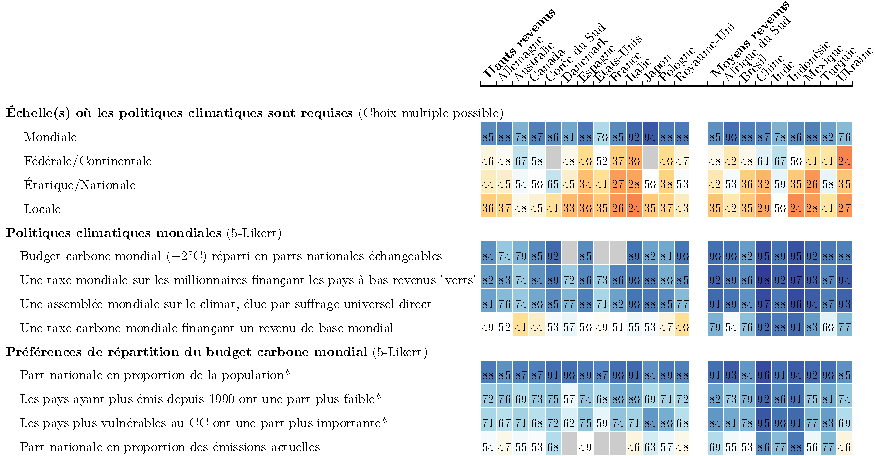
\includegraphics[width=\paperwidth]
  {../figures/OECD/Heatplot_global_tax_attitudes_share_fr.pdf}}\label{fig:oecd} % with dependence on others (absent from OECD): Heatplot_burden_share_all_share_countries
  {\footnotesize \\ $\quad$ \\ Note 1~: Pourcentage de réponses \textit{Très} et \textit{Plutôt favorable}, en excluant les réponses \textit{Indifférent\textperiodcentered{}e} ($n$ = 40,680). Source~: \citet{fabre_international_2023}. %The numbers represent the share of \textit{Somewhat} or \textit{Strongly support} among non-\textit{indifferent} answers (in percent, $n$ = 40,680). 
  La couleur bleue dénote une majorité relative. %The color blue denotes a relative majority. See Figure \ref{fig:oecd_absolute} for the absolute support. (Questions \ref{q:scale}-\ref{q:millionaire_tax}. Reproduced from \citealp{dechezlepretre_fighting_2022}, Figure A21.) 
  \\ Note 2~: *Au Danemark, en France et aux États-Unis, les questions avec une astérisque ont été posées différemment. %In Denmark, France and the U.S., the questions with an asterisk were asked differently, cf. Question \ref{q:burden_sharing_asterisk}. 
  } 
\end{figure}

La première de ces enquêtes a été réalisée sur 20 pays %avec le soutien de l'OCDE 
entre 2021 et 2022\footnote{Avec mes co-auteurs Antoine Dechezleprêtre, Tobias Kruse, Bluebery Planterose, Ana Sanchez-Chico et Stefanie Stantcheva, nous avons conduit une enquête sur les attitudes envers le changement climatique et les politiques climatiques. Cette enquête porte sur 20 pays couvrant 72~\% des émissions mondiales de CO$_\text{2}$ (plus ou moins les pays du G20), avec des échantillons représentatifs d'environ 2~000 répondants par pays. Elle avait pour but principal d'étudier les attitudes envers des politiques climatiques nationales, mais nous avons également posé quelques questions sur des mesures mondiales.}. Il s'est avéré que parmi les mesures climatiques les plus soutenues figurent trois mesures mondiales ayant chacune une forte dimension redistributive~: un quota de permis d'émissions échangeables, une assemblée mondiale élue démocratiquement qui proposerait un traité sur le climat, et un impôt mondial sur la fortune finançant les pays à bas revenus qui respectent les objectifs climatiques. Dans chaque pays, chacune de ces mesures obtient une majorité de soutien absolu\footnote{À une exception près~: l'assemblée mondiale pour le climat n'obtient \textit{que} 48~\% de soutien absolu aux États-Unis.} 
et plus de 70~\% de soutien relatif (c'est-à-dire en excluant les réponses \textit{Indifférent\textperiodcentered{}e}), 
comme le montre la Figure \ref{fig:oecd}. Ces résultats sont cohérents avec une autre question où l'on demandait à quelle(s) échelle(s) des politiques climatiques sont requises~: % PNON choix multiple
l'écrasante majorité a répondu l'échelle mondiale, tandis que l'échelle continentale ou nationale n'a été choisie que par une petite moitié des répondants. 

La question sur le quota mondial ne précisait pas l'allocation des permis d'émissions entre pays, mais la question suivante testait le soutien à cette mesure selon différentes variantes d'allocation des permis. En cohérence avec les préférences sur la répartition de l'effort révélées par les travaux sus-mentionnés, notre enquête met en évidence un consensus en faveur d'une allocation des permis au pro rata de la population des pays, ce qui correspond à la répartition égalitaire au cœur du Plan mondial pour le climat\footnote{En fait, c'est précisément suite à ce consensus que j'ai défini le Plan sur cette base égalitaire. Si ça ne tenait qu'à moi, j'aurais préféré une approche encore plus redistributive que l'égalitaire.}. Cette variante obtient entre 84~\% et 96~\% de soutien relatif selon les pays, et une majorité absolue de soutien dans tous les pays (même en incluant les réponses \textit{Indifférent\textperiodcentered{}e})\footnote{La variante la moins appréciée (mais qui récolte quand même une majorité de soutien relatif dans la plupart des pays) attribue les permis d'émissions en proportion des émissions actuelles, et n'implique ainsi aucune redistribution Nord--Sud. Un niveau de soutien intermédiaire (qui reste donc élevé) est obtenu par les variantes encore plus redistributives que l'option égalitaire~: celle tenant compte des responsabilités historiques en attribuant moins de permis aux pays qui ont plus émis par le passé, ou celle tenant compte de la vulnérabilité face au changement climatique en attribuant plus de permis aux pays qui subiront des préjudices plus importants.}.

Malgré le soutien extrêmement fort à un quota mondial égalitaire, une taxe carbone mondiale finançant un revenu de base mondial obtient un soutien bien plus faible, autour de 50~\% dans les pays à hauts revenus. Pourtant, les deux mesures sont équivalentes d'un point de vue économique dès lors que le prix du carbone est le même dans les deux systèmes, comme on l'a vu au Chapitre \ref{ch:coeur}\footnote{En effet, pourvu que le prix du carbone soit le même dans les deux systèmes, les consommateurs font face aux mêmes hausses de prix~; et le revenu de base répartit les recettes en proportion de la population adulte des pays.}. 
Deux facteurs expliquent cette différence dans le soutien. D'une part, les gens peuvent préférer un quota à une taxe, car dans le cas du quota, il est certain que les émissions seront réduites conformément à l'objectif. D'autre part, lors %lorsque nous avons posé la 
des questions sur la taxe carbone, %nous avons également informé les répondants 
les répondants avaient été informés 
du coût de ce système sur leur pouvoir d'achat. Sans une enquête complémentaire, nous ne pouvions pas connaître le taux de soutien au Plan mondial pour le climat (c'est-à-dire au quota égalitaire) lorsque les gens sont informés de la perte de pouvoir d'achat qu'il engendrerait\footnote{Les montants de ces pertes sont reportés aux notes \ref{fn15}-\ref{fn16} et la méthode de calcul en Annexe \ref{app:pays}.}.   

% De 70~\% (aux États-Unis) à 94~\% (au Japon) des personnes interrogées considèrent le niveau mondial comme l'échelle appropriée pour l'adoption de politiques climatiques. En revanche, le niveau européen est choisi par moins de la moitié des répondants européens, le niveau fédéral n'est choisi que par 52~\% des répondants américains, et les niveaux nationaux ou locaux sont choisis par un nombre encore plus restreint de personnes. Il n'est donc pas surprenant que 50~\% (au Japon) à 78~\% (en Chine et en Inde) %74~\% (en Allemagne) à 95~\% (en Chine et en Indonésie) 
% soutiennent le principe d'un système mondial d'échange de permis d'émission. 
% Il est intéressant de noter qu'avec un soutien d'au moins 84~\% dans chaque pays, avec un soutien absolu de 53~\% (au Japon) à 76~\% (en Chine), il existe un consensus mondial en faveur d'un système mondial d'échange de quotas d'émission qui attribue des permis d'émission proportionnellement à la population des pays, conformément à un droit d'émission égal pour chaque être humain. Dans tous les pays, cette solution est préférée à d'autres solutions, telles que l'octroi de droits d'émission supplémentaires aux pays qui ont moins émis dans le passé (\textit{responsabilités historiques}, deuxième option préférée dans l'ensemble), ou aux pays qui émettent actuellement plus (\textit{grandfathering}, option la moins préférée dans l'ensemble). 

\subsection{Fort soutien au Plan mondial pour le climat}

Pour comprendre en profondeur les attitudes envers le Plan mondial pour le climat, j'ai mené en 2023 une enquête complémentaire avec deux nouveaux co-auteurs~: Thomas Douenne et Linus Mattauch. Cette enquête repose sur un échantillon représentatif de 3~000 européens (en Allemagne, en Espagne, en France et au Royaume-Uni) et deux échantillons représentatifs de (respectivement) 3~000 et 2~000 États-uniens. 
% \begin{figure}[h !] 
%     \caption[]{Soutien au Plan mondial pour le climat à travers le monde (en pourcentage).}\label{fig:support}
%     \makebox[\textwidth][c]{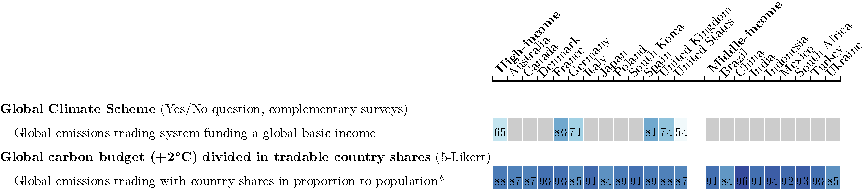
\includegraphics[width=1.2\textwidth]{../figures/OECD/Heatplot_global_tax_attitudes_only_GCS_share.pdf}} 
%     % \makebox[\textwidth][c]{\includegraphics[width=1.2\textwidth]{../figures/OECD/Heatplot_global_tax_attitudes_GCP_share.pdf}} 
% \end{figure}

Même en comprenant bien la baisse de pouvoir d'achat qu'il implique, 76~\% des Européens et 54~\% des Américains soutiennent le Plan mondial pour le climat (cf. Figure \ref{fig:gcs_support})
\footnote{\label{fn15}
Voici comment nous avons décrit la mesure aux répondants~:
\begin{quote}
En 2015, tous les pays se sont mis d'accord pour contenir le réchauffement climatique ``bien en-dessous de +2~\textdegree{}C''. Pour limiter le réchauffement climatique à ce niveau, \textbf{il existe une quantité maximale de gaz à effet de serre que nous pouvons émettre à l'échelle mondiale}. \\
Pour respecter cet objectif climatique, on peut créer des permis d'émission de gaz à effet de serre en nombre limité à l'échelle mondiale. Les entreprises polluantes seraient tenues d'acheter des permis pour couvrir leurs émissions. Une telle politique \textbf{obligerait les compagnies pétrolières à payer} leurs émissions et augmenterait progressivement le prix des combustibles fossiles. \textbf{Des prix plus élevés encourageraient les ménages et les entreprises à utiliser moins de combustibles fossiles, réduisant ainsi les émissions de gaz à effet de serre.} \\
Conformément au principe selon lequel chaque être humain a un droit égal à polluer, les revenus générés par la vente de permis pourraient financer un revenu de base mondial. \textbf{Chaque adulte recevrait 30~\euro{} par mois}, sortant ainsi de l'extrême pauvreté les 700 millions de personnes qui gagnent moins de 2~\textit{\$} par jour. \\
~[\textbf{Le Français}]\textbf{ type perdrait financièrement }[\textbf{10~\euro{}}]\textbf{ par mois}\footnotemark{\label{fn16}} 
% \footnote{Ce coût mensuel net médian est ajusté suivant le pays. Il est de 85\$ aux États-Unis, 25\euro{} en Allemagne, 5\euro{} en Espagne et 20£ au Royaume-Uni.} 
(car il ferait face à [40~\euro{}] par mois d'augmentations de prix, ce qui est supérieur aux 30~\euro{} qu'il recevrait). \\
La mesure pourrait être mise en place dès que des pays qui totalisent plus de 60~\% des émissions mondiales s'accordent dessus. Les pays qui refuseraient de participer à la mesure pourraient faire face à des sanctions (comme des droits de douane) du reste du monde et seraient exclus du revenu de base.
\end{quote}
Nous nous sommes ensuite assurés que les répondants avaient retenu qui gagnerait ou perdrait suite à cette mesure, et notamment qu'elle serait coûteuse pour les personnes typiques de leur pays. Pour ce faire, nous avons posé des questions de compréhension, puis affiché la réponse correcte. Enfin, nous avons décrit la mesure à nouveau, de façon plus succincte, avant de tester le soutien à l'aide d'une question Oui/Non.}. 
\footnotetext{\label{fn16}Ce coût mensuel net médian est ajusté suivant le pays. Il est de 85~\$ aux États-Unis, 25~\euro{} en Allemagne, 5~\euro{} en Espagne et 20~£ au Royaume-Uni.} 
En Europe, quel que ce soit le pays ou le positionnement politique, une large majorité soutient le Plan mondial pour le climat. 
Aux États-Unis, il y a une forte polarisation~: 74~\% des électeurs de Biden soutiennent le Plan tandis que 74~\% des électeurs de Trump s'y opposent, les abstentionnistes le soutenant à 53~\%.  
Ces résultats montrent que la plupart des Occidentaux sont disposés à perdre quelques dizaines d'euros par mois si cela permet de mettre fin au changement climatique et à l'extrême pauvreté\footnote{Le soutien est plus important pour le quota que pour une taxe carbone (testée dans l'enquête sur 20 pays), ce qui confirme que la population préfère une mesure dont elle est certaine qu'elle réduira suffisamment les émissions de CO$_\text{2}$.}. 
% Pour évaluer la robustesse du soutien public constaté dans les 20 pays, \citet{fabre_international_2023} ont mené des enquêtes complémentaires auprès de 3~000 répondants américains et de 3~000 répondants européens (en France, en Allemagne, en Espagne et au Royaume-Uni). Ils décrivent le Plan en détaillant les effets négatifs sur le pouvoir d'achat des personnes interrogées. Malgré l'emphase sur ses coûts, le Plan obtient toujours un soutien majoritaire de 54~\% aux États-Unis et de 76~\% en Europe. À l'aide d'une technique appelée <<~expérience de liste~>>, ils démontrent en outre que ce soutien est authentique et n'est pas motivé par un éventuel biais de désirabilité sociale. En fait, une majorité de personnes dans chaque pays est prête à signer une pétition en faveur du Plan, sachant que la part des répondants prêts à signer sera transmise au cabinet du chef de l'État. 

\begin{figure}[h!]
  \caption[Soutien au Plan mondial pour le climat]{Soutien au Plan mondial pour le climat (pourcentage de \textit{Oui}).} 
  \makebox[\textwidth][c]{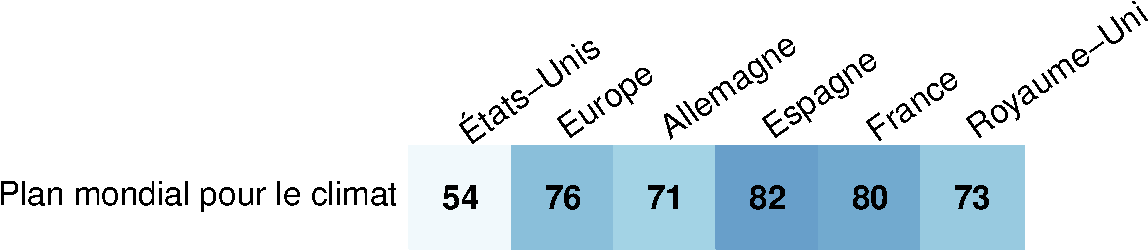
\includegraphics[width=1\textwidth]
  {../figures/FR/gcs_support_positive.pdf}}\label{fig:gcs_support} 
\end{figure}

\subsection{Un soutien authentique} % Authenticité?

Malgré des réponses très favorables au Plan, on pourrait douter du soutien déclaré. 
%Peut-être que les répondants font preuve d'un biais de désirabilité sociale~: ils disent soutenir le Plan car c'est ce qui semble la réponse attendue, les faisant apparaître comme altruistes, même si au fond d'eux ils s'opposent à cette mesure qui nuirait à leur confort et à leur pouvoir d'achat. Peut-être que le résultat serait différent si un référendum avait lieu sur la question (soit que les opinions changent suite au débat médiatique, soit que certaines personnes défendent leur intérêt personnel financier lorsque le choix revêt un véritable enjeu). Peut-être enfin que la plupart des gens soutiennent le Plan mondial pour le climat, mais n'attachent pas à la justice climatique une importance suffisante pour que cette question détermine leur vote aux élections. Par exemple, des personnes qui s'opposent à l'immigration et soutiennent une action climatique ambitieuse pourraient voter pour un parti nationaliste plutôt qu'un parti écologiste si la question de l'immigration est prioritaire pour elles. 
La seule façon d'être absolument certain qu'une majorité de la population soutient sincèrement le Plan serait d'organiser un référendum. Cela dit, même à l'aide d'une simple enquête, on peut avoir une bonne indication de la sincérité des réponses, et nous avons utilisé plusieurs méthodes pour tester cette sincérité dans la suite de l'enquête.

Pour approcher du mieux qu'on peut l'enjeu que constituerait un référendum, nous avons demandé aux répondants s'ils seraient prêts à signer une pétition en faveur du Plan mondial pour le climat, en sachant que les résultats à cette question (posée à un échantillon représentatif de la population) seraient transmis au cabinet du chef d'État. Ainsi, les répondants comprenaient que leur réponse pouvait avoir une influence sur la politique officielle. Aux États-Unis, une majorité est prête à signer la pétition et la différence avec le soutien déclaré direct n'est pas significative. En Europe, 69~\% des répondants seraient prêts à signer la pétition~: c'est certes 7 points de moins que pour le soutien déclaré, mais ça reste une large majorité. 

À l'aide d'une technique appelée <<~expérience de liste~>>, nous montrons que le soutien est authentique et n'est pas motivé par un éventuel biais de désirabilité sociale. Cette expérience fonctionne de la manière suivante~: nous demandons aux répondants \textit{combien} de mesures ils soutiennent parmi une liste de mesures, et nous ne savons donc pas si un répondant soutient telle ou telle mesure\footnote{De ce fait, les répondants ne font plus face à un biais de désirabilité sociale les incitant à mentir sur leur soutien à telle ou telle mesure.}. 
Pour une moitié aléatoire des répondants, nous ajoutons le Plan mondial pour le climat dans la liste des mesures\footnote{En Europe, les trois autres mesures qui figurent dans les listes sont~: la peine de mort pour les crimes majeurs, un plan de redistribution nationale et un plan d'isolation thermique des bâtiments.}. 
En calculant la différence entre le nombre moyen de mesures soutenues dans les groupes avec et sans le Plan dans leur liste, on estime le soutien tacite au Plan\footnote{Par exemple, si le \textit{groupe sans} le Plan soutient en moyenne 2,1 mesures, et le \textit{groupe avec} en soutient 2,86, on peut faire l'hypothèse que le \textit{groupe avec} le Plan soutient autant les autres mesures que le \textit{groupe sans} (puisqu'ils sont chacuns représentatifs de la population), et que la différence entre le nombre de mesures soutenues correspond au soutien au Plan, soit $2,86 - 2,1 = 76~\%$ de soutien tacite en faveur du Plan mondial pour le climat.}. % PTET? mettre vrais chiffres? - 1.49 = 72% en UE / - 1.15 = 52% aux US
% Pour un groupe aléatoire de répondants, la liste contient trois mesures\footnote{En Europe, les trois mesures que nous avons employées sont~: la peine de mort pour les crimes majeurs, un plan de redistribution nationale et un plan d'isolation thermique des bâtiments.}. Pour un autre groupe aléatoire de répondants, la liste contient quatre mesures~: les trois mesures précédentes ainsi que la mesure qui nous intéresse, le Plan mondial pour le climat. % PTET on vs. nous
% Comme on demande seulement aux répondants \textit{combien} de mesures ils soutiennent, on ne sait pas quelles mesures un répondant donné soutient. Pour cette raison, les répondants ne font plus face à un biais de désirabilité sociale les incitant à mentir sur leur soutien à telle ou telle mesure. Par ailleurs, cette méthode permet quand même d'estimer le soutien à la mesure qui nous intéresse, en calculant la différence entre le nombre moyen de mesures soutenues dans le groupe avec la liste à quatre mesures et celui de la liste à trois mesures\footnote{Par exemple, si le groupe à trois mesures en soutient en moyenne 2,1, et le groupe à quatre mesures 2,86, on peut faire l'hypothèse que le groupe à quatre mesure soutient autant les trois premières mesures que l'autre groupe (puisqu'ils sont chacuns représentatifs de la population), et que la différence entre le nombre de mesures soutenues correspond au soutien à la quatrième mesure, soit $2,86 - 2,1 = 76~\%$ de soutien tacite en faveur du Plan mondial pour le climat.}. On peut alors estimer le biais de désirabilité sociale en comparant le soutien tacite au soutien déclaré à la question directe, rapporté précédemment
% \footnote{Dans d'autres contextes, cette méthode a révélé un biais de désirabilité sociale en faveur de l'invasion de l'Ukraine parmi la population russe (le soutien tacite étant 10 à 20 points plus faible que le soutien déclaré), ou encore la sous-déclaration d'opinions racistes dans le Sud des États-Unis \citep{kuklinski_racial_1997,chapkovski_solid_2022}.}. 
% Dans notre enquête, l
Le soutien tacite n'est pas significativement différent du soutien déclaré, ce qui indique que les répondants ne font pas semblant %feignent pas 
de soutenir le Plan en vue de satisfaire une norme sociale%est authentique et n'est pas motivé par un éventuel biais de désirabilité sociale
\footnote{Dans d'autres contextes, cette méthode a révélé un biais de désirabilité sociale en faveur de l'invasion de l'Ukraine au sein de la population russe (le soutien tacite étant 10 à 20 points plus faible que le soutien déclaré), ou encore la sous-déclaration d'opinions racistes dans le Sud des États-Unis \citep{kuklinski_racial_1997,chapkovski_solid_2022}.}. 

\subsection{Un gain électoral à faire campagne pour le Plan}
La preuve la plus convaincante que le soutien au Plan est profond est qu'un candidat progressiste pourrait gagner des voix en le soutenant. Nous le montrons à travers différentes questions. Tout d'abord, nous décrivons un programme progressiste et un programme conservateur correspondant aux programmes typiques des principaux partis du pays\footnote{Nous présentons le choix entre les deux programmes comme étant celui entre les deux candidats de la prochaine élection majeure (en France, le second tour de la prochaine élection présidentielle), puis nous demandons aux personnes interrogées pour quel candidat elles voteraient.}. Pour une moitié aléatoire de l'échantillon, nous ajoutons le Plan mondial pour le climat au programme progressiste. En France, le candidat progressiste gagnerait 11 points de vote en incluant le Plan dans son programme. Aux États-Unis, le candidat progressiste pourrait gagner 3 points, tandis que dans les autres pays, l'effet n'est pas significativement différent de zéro\footnote{Le gain électoral est très significatif en France (la valeur $p$ est de 0,5~\%). Pour les États-Unis, la valeur $p$ est de 13~\%, c'est-à-dire non statistiquement significative au seuil habituel de 5~\%, mais avec seulement 13~\% de chances que le candidat progressiste n'ait aucun gain électoral en soutenant le Plan. Pour les autres pays, le gain électoral n'est pas significativement différent de zéro (même au seuil de 20~\%).}. 
%
Ainsi, le soutien au Plan mondial pour le climat ne ferait perdre des voix à un candidat progressiste dans aucun pays, et pourrait rapporter un gain électoral important en France. 

Dans la question suivante, nous tirons au sort deux programmes politiques à partir d'un ensemble de mesures (plutôt progressistes), puis nous ajoutons le Plan à l'un des programmes\footnote{En Europe, les personnes interrogées sont invitées à imaginer qu'une coalition de gauche ou de centre-gauche remportera les prochaines élections et il leur est demandé sur quel programme elles préféreraient que cette coalition ait été élue. Aux États-Unis, la question est formulée comme un duel hypothétique dans une primaire démocrate et n'est posée qu'aux non-républicains (c'est-à-dire aux démocrates, aux indépendants et aux non-affiliés).}. Le programme contenant le Plan est systématiquement préféré par une majorité (allant de 58~\% aux États-Unis et au Royaume-Uni à 64~\% en Espagne, cf. Figure \ref{fig:conjoint_left_ag_b}). Cette question et la précédente révèlent que le soutien au Plan mondial pour le climat est non seulement sincère, mais est aussi suffisamment important pour déterminer le choix électoral de certains électeurs\footnote{
% Enfin, cette priorisation du Plan est confirmée 
Cet intérêt pour 
% Cette priorisation de 
la redistribution mondiale est confirmé lors d'une question demandant aux répondants de répartir 100 points pour exprimer leur soutien à un ensemble de mesures (les mêmes que précédemment), avec la consigne d'attribuer davantage de points aux mesures qu'ils soutiennent le plus. Le Plan mondial pour le climat est plus priorisé que la moyenne et fait partie des politiques climatiques les plus appréciées. À l'inverse, une mesure climatique promulguée dans l'UE et en Californie (l'élimination progressive des voitures thermiques neuves) est l'une des trois mesures les moins priorisées dans chaque pays. Plus généralement, cette question montre que les mesures de redistribution mondiales sont assez prioritaires pour l'électorat, juste derrière les mesures les plus appréciées~: l'augmentation du salaire minimum et l'amélioration des services publics grâce à des financements supplémentaires pour l'éducation et la santé.}. 

\begin{figure}[h!] 
  \caption[Influence du Plan sur le programme préféré]{Influence du Plan sur le programme préféré~:\\ Préférence pour un programme aléatoire A contenant le Plan mondial pour le climat plutôt qu'un programme B ne le contenant pas (en \%). (Aux États-Unis, question posée uniquement aux non-Républicains).}\label{fig:conjoint_left_ag_b}
  \makebox[\textwidth][c]{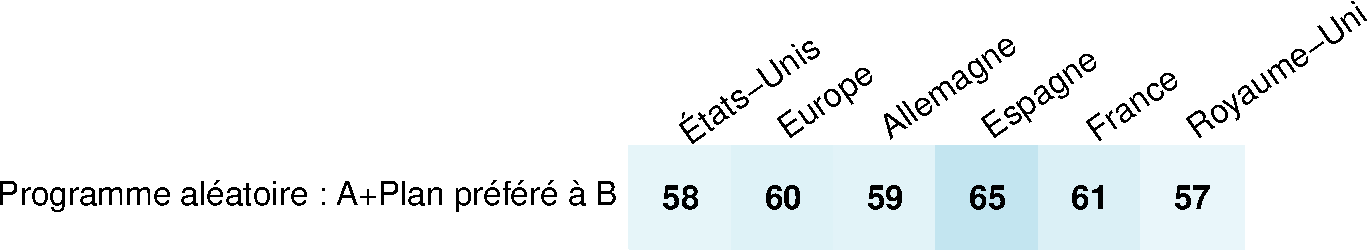
\includegraphics[width=\textwidth]{../figures/FR/conjoint_left_ag_b_binary_positive.pdf}} 
\end{figure}


Pour résumer, les enquêtes d'opinion révèlent un soutien majoritaire large et sincère en faveur du Plan mondial pour le climat, et indiquent que la population préfère les programmes politiques qui incluent cette mesure plutôt que les programmes qui ne la contiennent pas. Et ce, alors même que les répondants occidentaux sont pleinement conscients qu'ils perdraient un peu de pouvoir d'achat dans le cadre du Plan mondial pour le climat. 

Si la population soutient ce Plan, c'est parce qu'il est équitable et mondial, donc effectif pour mettre fin au changement climatique. Ce n'était pas le cas de la taxe carbone française contre laquelle se sont opposés les Gilets jaunes, et dont on a clairement mesuré le rejet dans les enquêtes d'opinion. En d'autres termes, la plupart des gens sont préoccupés par le climat, et disposés à soutenir une solution pour peu qu'elle soit juste et effective. 
Pour en savoir plus sur ces enquêtes% (lire le questionnaire, les méthodes précises et les résultats complets)
, je renvoie le lecteur à l'article académique intitulé \textit{International Attitudes Toward Global Policies}, que j'ai co-écrit avec Thomas Douenne et Linus Mattauch. 

\chapter*{\textit{Déroulé du futur politique rêvé}}\label{ch:narr_reve}
\addcontentsline{toc}{chapter}{\nameref{ch:narr_reve}} 

L'année de ma naissance a eu lieu la première conférence sur le changement climatique. On est alors en 1992 et des économistes imaginent déjà ce qui deviendra plus tard le Plan mondial pour le climat. Une idée balayée par les États-Unis lors de la négociation du protocole de Kyoto, mais qui suscite un regain d'intérêt lorsqu'une étude financée par l'OCDE révèle en 2023 que près 80~\% de la population soutiendrait ce Plan dans tous les pays. Démarre alors un marathon de plaidoyer, d'abord auprès des économistes, faciles à convaincre, puis des associations, difficiles à joindre, 
et enfin auprès du monde politique. Au moment où j'écris, ce Plan a déjà obtenu la bénédiction de plusieurs prix Nobel, nous l'avons présenté au cabinet du Président de la République, et des partis politiques réfléchissent à l'intégrer dans leur programme. Voici l'Histoire que nous pouvons écrire ensemble, pour mettre un terme au changement climatique et à l'extrême pauvreté. 

~[début de la fiction] La présidence brésilienne du G20 soumet l'idée lors du sommet de 2024. Elle est immédiatement soutenue par Greta Thunberg et Antonio Guterres, le secrétaire général de l'ONU. 
En coulisses, Wang Yi, le ministre chinois des affaires étrangères, discute du Plan avec son homologue européen, Josep Borrell. 
% Dans les coulisses, les commissaires européens aux relations extérieures et à l'économie, Josep Borrell et Paolo Gentiloni, discutent du plan avec Huang Runqiu et Wang Yi, ministres chinois de l'environnement et des affaires étrangères. 
Même si les tractations restent secrètes, la gauche européenne décide de faire campagne sur ce Plan lors des élections de 2024. Contre toute attente, elle les remporte haut la main. Tout s'emballe. En novembre 2024, le Brésil, l'Union Européenne, la Chine et l'Inde font de ce plan leur position commune lors de la COP29. Suite à la réélection de Donald Trump, les États-Unis refusent évidemment cet accord, mais les gouverneurs de Californie et de l'État de New York font savoir que leurs États rejoindront l'accord, même si le niveau fédéral ne suit pas. Les pays africains n'en croient pas leurs yeux~: 
% est-ce que la plupart des pays vont vraiment s'accorder 
% la plupart des pays vont-ils vraiment s'accorder 
va-t-on vraiment obtenir un accord international %de la plupart des pays 
sur un plan qui doublerait le revenu moyen d'un pays comme le Burundi, en versant à chaque humain un revenu de base de 40~\euro{}/mois~? En février 2025, un groupe de 156 pays et 9 États états-uniens, couvrant 74~\% des émissions de CO$_\text{2}$ mondiales, signent un accord de principe pour négocier le plafonnement de leurs émissions de CO$_\text{2}$. S'ensuit une bataille de cinq longues années pour négocier ce plan, puis une implémentation laborieuse, qui prendra du retard, mais sera pleinement opérationnelle en 2037. Dopée par le revenu de base, l'Afrique connaît alors un boom économique sans précédent. Dans les années 2050, les États-Unis et la Russie finissent par rejoindre le club climatique. L'Arabie Saoudite est le dernier pays à franchir le pas, en 2061. En 2084, le monde entier a atteint la neutralité carbone, et plus personne ne vit avec moins de 8 dollars par jour. Ce n'était pas gagné~: la moitié de l'humanité vit sous ce seuil de pauvreté à l'heure où j'écris ces lignes. % 50% < 8$ according to World Bank's pretax (less if we use WID or posttax): 57% < 10$
Et vous, grévistes --- je suis sûr que vous en êtes, vous n'y êtes pas pour rien. En effet, rien de tout cela n'aurait pu aboutir sans la grève mondiale pour le climat d'octobre 2024, suivie par près d'un milliard de personnes.

\chapter{Les grands éléments du Plan mondial pour le climat\label{ch:principes}}

La proposition développée dans ce chapitre ne résout pas tous les problèmes de l'humanité, et ne constitue pas non plus une réponse complète au changement climatique. Bien qu'elle soit désignée <<~Plan mondial pour le climat~>> (parce que ça sonne bien), <<~Cadre international de sortie des énergies fossiles~>> aurait été plus fidèle.  % Une désignation telle que <<~Cadre international de sortie des énergies fossiles~>> aurait été plus fidèle, mais il faut dire que <<~Plan mondial pour le climat~>> sonne mieux. %C'est donc peut-être exagéré de le nommer <<~Plan mondial pour le climat~>>, mais ça sonne mieux qu'une désignation plus fidèle telle que <<~Cadre international de sortie des énergies fossiles~>>. 
En effet, en l'état actuel, ce Plan couvre uniquement les émissions de CO$_\text{2}$ fossiles et industrielles, pas celles liées à l'usage des terres, à la forêt ou aux autres gaz à effet de serre. % PTET? Inclure toutes émissions ? mettre ça dans Ch 3?
Sa portée se limite à établir un traité-cadre qui garantit les réductions d'émissions et détermine les transferts internationaux. Charge ensuite à chaque État ou collectivité de prendre les mesures (climatiques et sociales) appropriées pour que la décarbonation se passe bien sur son territoire. Son champ d'application étant posé, % Ses limitations / Son périmètre
examinons les grands principes du Plan.

\section{1$^\text{er}$ principe~: Un quota annuel d'émissions}\label{sec:pcp_quota}

Le budget carbone --- et avec lui le climat futur --- est l'élément décisif que les États devront négocier. 
Notre proposition repose sur un budget d'émissions nettes et couvre la période où les émissions nettes sont positives, c'est-à-dire où les émissions excèdent la séquestration (cf. ci-après). La Figure \ref{fig:emissions_par_region} illustre une trajectoire mondiale d'émissions sur laquelle les pays pourraient s'accorder et projette les trajectoires qu'elle pourrait impliquer dans différentes régions (cf. détails en Annexe \ref{app:pays}). 

\begin{figure}[h!]
  \caption[Trajectoires d'émissions par région]{Trajectoires estimées des émissions de CO$_\text{2}$ par adulte dans différentes régions pour un scénario +1,8\textdegree{}C.}\label{fig:emissions_par_region}
  \makebox[\textwidth][c]{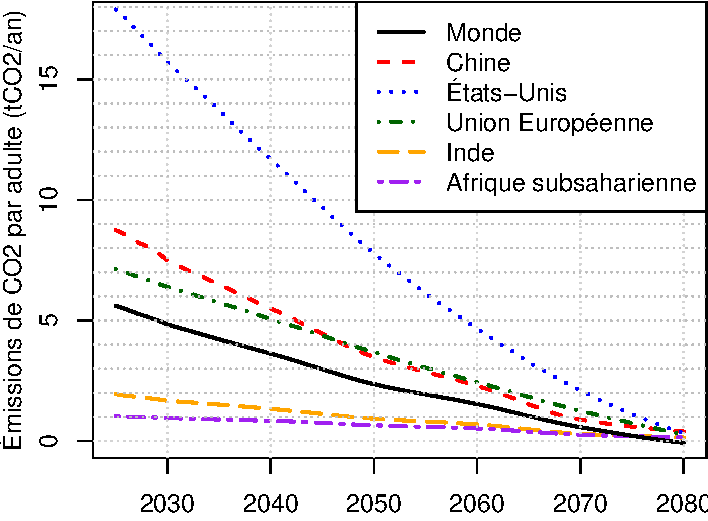
\includegraphics[width=.92\textwidth]{../figures/policies/emissions_par_region_sm.pdf}} % .92
\end{figure} 

Le marché carbone fonctionne de la façon suivante. 
L'organe de gouvernance du Plan définit le quota annuel d'émissions, selon une trajectoire conforme au budget carbone. En début d'année, ce quota est mis aux enchères. %sous la forme de permis d'émissions d'une tonne de CO$_\text{2}$. 
Les sociétés assujetties sont les entreprises \textit{upstream}, c'est-à-dire celles qui mettent sur le marché des hydrocarbures (charbon, pétrole, gaz) ou dont les procédés industriels émettent du CO$_\text{2}$ (production de ciment, d'hydrocarbures, incinérateurs\dots). 
% Les sociétés assujetties sont les entreprises ``upstream'', c'est-à-dire celles qui extraient des hydrocarbures, importent des biens depuis des pays non participants, ou produisent du ciment\footnote{L'assujettissement pourrait s'opérer un peu plus en aval dans la chaîne de valeur (``midstream''), au niveau des dépôts d'hydrocarbures. Cela permettrait de ne pas faire payer la production de plastique, qui n'engendre pas directement des émissions, et de bénéficier de l'administration existante des droits d'accise sur les produits pétroliers.}. 
Chaque société assujettie annonce la quantité de permis qu'elle s'engage à acheter pour chaque niveau de prix du carbone. Pour chaque prix possible, on obtient ainsi une quantité agrégée demandée par les sociétés assujetties, qui décroît avec le prix. Les permis d'émissions sont alors vendus au prix pour lequel la quantité agrégée demandée correspond au quota. Les sociétés assujetties et des sociétés financières agréées peuvent ensuite échanger des permis d'émissions sur un marché secondaire. Au bout de quelques années (probablement une ou deux), le prix d'équilibre aura été découvert, de sorte que le prix sur le marché secondaire sera relativement stable et égal à celui des enchères. En fin d'année, les émissions issues des entreprises assujetties sont contrôlées, et ces entreprises doivent délivrer des permis à hauteur de leurs émissions. % les entreprises assujetties doivent alors restituer des permis d'émission à la même hauteur que leurs émissions constatées.
Des sanctions dissuasives garantissent le bon fonctionnement du système. Par exemple, pour toute tonne de CO$_\text{2}$ émise mais non couverte par un permis d'émissions, la société fautive doit payer une amende égale à trois fois le prix d'une tonne de CO$_\text{2}$, et doit toujours délivrer le permis manquant l'année suivante. En outre, un pays risque l'exclusion du système s'il ne fait pas appliquer correctement le Plan sur son territoire. % BOF réécrire paragraphe

En résumé, un système d'échange de permis d'émission (ETS, pour \textit{emissions trading system}) serait mis en place pour plafonner les émissions de CO$_\text{2}$ à l'échelle internationale. 
Un tel système a déjà fait ses preuves dans plusieurs pays, dont l'Union Européenne\footnote{L'ETS européen est souvent décrié. Pourtant, il a bel et bien permis de réduire les émissions couvertes (celles de l'industrie et de la production d'électricité) conformément à l'objectif fixé, tandis que les émissions non couvertes (mais qui le seront à partir de 2027) ont continué de croître. En réalité, l'ETS européen a été critiqué pour deux (bonnes) raisons. D'une part, l'objectif fixé n'était pas assez ambitieux (c'est ce qui explique le prix très faible jusqu'à une réforme du système en 2019). D'autre part, les permis d'émissions étaient attribués gratuitement aux entreprises polluantes, plutôt que vendus aux enchères. Ces deux écueils sont évités dans le Plan mondial pour le climat.}, la Chine et la Corée du Sud, et est à l'étude dans d'autres comme l'Inde, le Brésil ou le Nigeria. 17~\% des émissions mondiales sont déjà couvertes par un ETS. En outre, différents ETS peuvent être fusionnés avec succès, comme l'ont montré la Californie et le Québec \citep{icap_emissions_2023}. Dans le cas du Plan proposé, le nouvel ETS viendrait s'ajouter aux ETS existants plutôt que fusionner avec eux, pour éviter de réduire l'ambition de certains d'entre eux. En particulier, l'ETS européen a une trajectoire de décarbonation rapide, puisqu'à partir de 2040, plus aucun permis d'émission ne sera créé pour l'électricité et les grandes installations industrielles\footnote{\cite{pahle_emerging_2023}.}. Au passage, la décarbonation en cours dans l'UE montre que le marché du carbone fonctionne comme prévu.

\paragraph{Les émissions négatives}
Pour séquestrer du carbone présent dans l'atmosphère, plusieurs méthodes sont possibles, dont la reforestation (et plus généralement, les gains de biomasse), la bioénergie avec captage et stockage du CO$_\text{2}$\footnote{Le BECCS consiste à cultiver des plantes, à les incinérer (ce qui au passage fournit de l'énergie), à récupérer l'essentiel du CO$_\text{2}$ dans les cheminées de l'usine, puis à séquestrer ce CO$_\text{2}$ dans des cavités souterraines.} (BECCS), ou encore le captage direct du CO$_\text{2}$\footnote{Les technologies de captage direct (ou \textit{direct air capture}) permettent d'extraire le CO$_\text{2}$ de l'air à l'aide d'un solvant liquide ou d'un absorbant solide.}. Pour atteindre la cible de 1,5\textdegree{}C en 2100, de telles émissions négatives seront nécessaires, surtout à la fin du siècle, lorsque les actions de décarbonation plus abordables auront été effectuées\footnote{\cite{minx_negative_2018}.}. 

Dans ce livre, nous interprétons l'accord de Paris comme permettant un dépassement temporaire de la cible de 1,5\textdegree{}C dès lors que le réchauffement n'excède pas 2\textdegree{}C. En d'autres termes, des émissions négatives nettes (à partir de la deuxième moitié de ce siècle) permettront de redescendre jusqu'à 1,5\textdegree{}C, seuil qui sera très probablement déjà franchi en 2040\footnote{\citet{diffenbaugh_data-driven_2023} estiment que le réchauffement dépassera 1,5\textdegree{}C en 2035 dans un scénario de décarbonation ambitieuse, ce qui est cohérent avec la Table 4.2 du rapport de l'\citet{ipcc_climate_2021}.}. 
Pour fixer les idées, disons que le budget d'émissions positives serait de 1~000 GtCO$_\text{2}$ à partir de 2025. Ce budget carbone est conforme à l'objectif de ne pas dépasser les 2\textdegree{}C de réchauffement\footnote{Plus précisément, il y a deux chances sur trois de ne pas dépasser les 2\textdegree{}C de réchauffement avec un budget carbone de 1~000 GtCO$_\text{2}$ à partir de 2024.}. 
Dans la phase suivante, où les émissions nettes seront négatives, il y aurait deux budgets carbone annuels~: un quota d'émissions positives résiduelles (pour les activités impossibles à décarboner), et une commande d'émissions négatives. Un appel d'offre annuel permettrait d'acheter ces émissions négatives au moindre coût, et cette séquestration du carbone serait financée par des taxes sur les plus riches, telles qu'un impôt mondial sur la fortune
\footnote{Seuls les projets dont la séquestration est indiscutable seraient financés. Ainsi, la séquestration par gain de biomasse forestière ne serait financée que si les émissions liées à la perte de biomasse forestière sont tarifées par ailleurs. La séquestration du carbone pourrait être financée dès la première phase, là aussi à travers des taxes sur les plus riches. Sa valeur serait alors fixée au prix de marché, et la séquestration ainsi rémunérée viendrait gonfler d'autant le quota d'émissions mis aux enchères.}. % PS : après réflexion, je préfère le système où les crédits pour la séquestration carbone sont séparés du marché du carbone. Ils seraient rémunérés au prix de marché du carbone (et on pourrait également prévoir des subventions pour la R&D et des projets pilote). La séquestration rémunérée par l'UE pourrait venir gonfler d'autant le quota d'émissions mis aux enchères. Mais la séquestration devrait être rémunérée par d'autres ressources que les recettes de l'ETS (par exemple, un impôt sur la fortune). La raison de ma préférence pour cet arrangement est que l'intégralité des recettes liées aux émissions pourra être remise aux ménages (sous forme de transferts directs, de subventions et d'investissements) et le coût de la séquestration pourra reposer sur les plus riches (à travers un impôt affecté). Ça éviterait de se retrouver dans une situation ou une grosse part des recettes de l'ETS est captée par les entreprises de séquestration, et où on ne pourrait pas compenser les ménages pour les hausses de prix.
Au bout de quelques décennies d'émissions nettes négatives, on atteindrait la cible climatique de l'accord de Paris (1,5\textdegree{}C de réchauffement), et on pourrait même continuer de séquestrer du carbone pour atteindre un climat plus clément et limiter la hausse du niveau de la mer. Dans ce livre, nous ne nous préoccupons pas des émissions négatives, qui ne prendront de l'ampleur que dans quelques décennies, et nous nous concentrons sur la première phase du Plan. 
% Notre proposition repose sur différents budgets carbone~: un budget d'émissions positives, conforme à l'objectif de ne pas dépasser les 2\textdegree{}C de réchauffement, et un budget d'émissions négatives, permettant de réduire la température. Pour fixer les idées, disons que le budget d'émissions positives serait de 1~000 GtCO$_\text{2}$ à partir de 2025, et le budget d'émissions négatives serait de 500 GtCO$_\text{2}$, ce qui signifie que le budget d'émissions nettes serait de $1~000-500=500$ GtCO$_\text{2}$. Pour l'instant, ne nous préoccupons pas des émissions négatives, qui ne prendront leur essor quand dans quelques décennies. 
% Faire différemment pour gérer le plastique : budget carbone jusqu'à net zéro, puis double budget (positif et négatif)
% Pb du plastique: si on le fait payer à l'extraction, on a intérêt à extraire, stocker sous forme de plastiques, et brûler plus tard quand la tonne est plus chère. Comment faire ?

\section{2$^\text{e}$ principe~: Un revenu de base mondial}\label{pcp:rdb}

Les recettes du Plan serviraient à financer un revenu de base mondial~: un même transfert à tous les humains de 15 ans ou plus\footnote{En réalité, il vaudrait mieux verser également un revenu de base aux (mères des) enfants de moins de 15 ans, d'un montant inférieur --- disons de moitié --- à celui reçu par les adultes. Ce livre modélise l'option sans revenu de base pour les enfants pour rester en phase avec la question posée dans l'enquête.%uniquement pour simplifier l'exposition
}. 
Nous estimons que le revenu de base s'élèverait à environ 50~\$ par mois entre 2030 et 2060\footnote{Le revenu de base est estimé en multipliant le prix du carbone par les émissions mondiales et en divisant le tout par la population adulte mondiale. Les personnes les plus attentives noteront que ce montant est plus élevé que celui utilisé dans l'enquête (30~\$ en 2030, cf. \citealp{fabre_global_2023}). En effet, pour ce livre, j'ai refait les calculs à l'aide d'un modèle plus sophistiqué (cf. Annexe \ref{app:pays}), et le prix du carbone qui est en issu est plus élevé que celui de ma source initiale \citep{stern_report_2017}.} (cf. Figure \ref{fig:trajectory}), 
ce qui suffirait à sortir de l'extrême pauvreté les 700 millions de personnes qui vivent avec moins de 2~\textit{\$} par jour. À leur apogée en 2030, les recettes du Plan sont estimées à 2~\% du PIB mondial. Le Plan entraînerait des transferts internationaux d'environ 0,6~\% % 0,9\%
du PIB mondial, le reste % 65~\% 
des recettes étant reversées dans le pays où elles sont perçues. Les effets distributifs du Plan sont détaillés au Chapitre \ref{ch:effets_distributifs}. %En utilisant un scénario limitant le réchauffement climatique à 1,8\textdegree{}C, n
% Même si les recettes diminueront lorsque la décarbonation sera presque achevée (vers les années 2060), le revenu de base mondial devrait être maintenu grâce à de nouvelles sources de financement (par exemple, un impôt mondial sur les bénéfices des sociétés). 

\begin{figure}[h!]
  \caption[Trajectoires (émissions, prix, revenu de base)]{Trajectoires estimées des émissions, du prix du carbone et du revenu de base.}\label{fig:trajectory}
  \makebox[\textwidth][c]{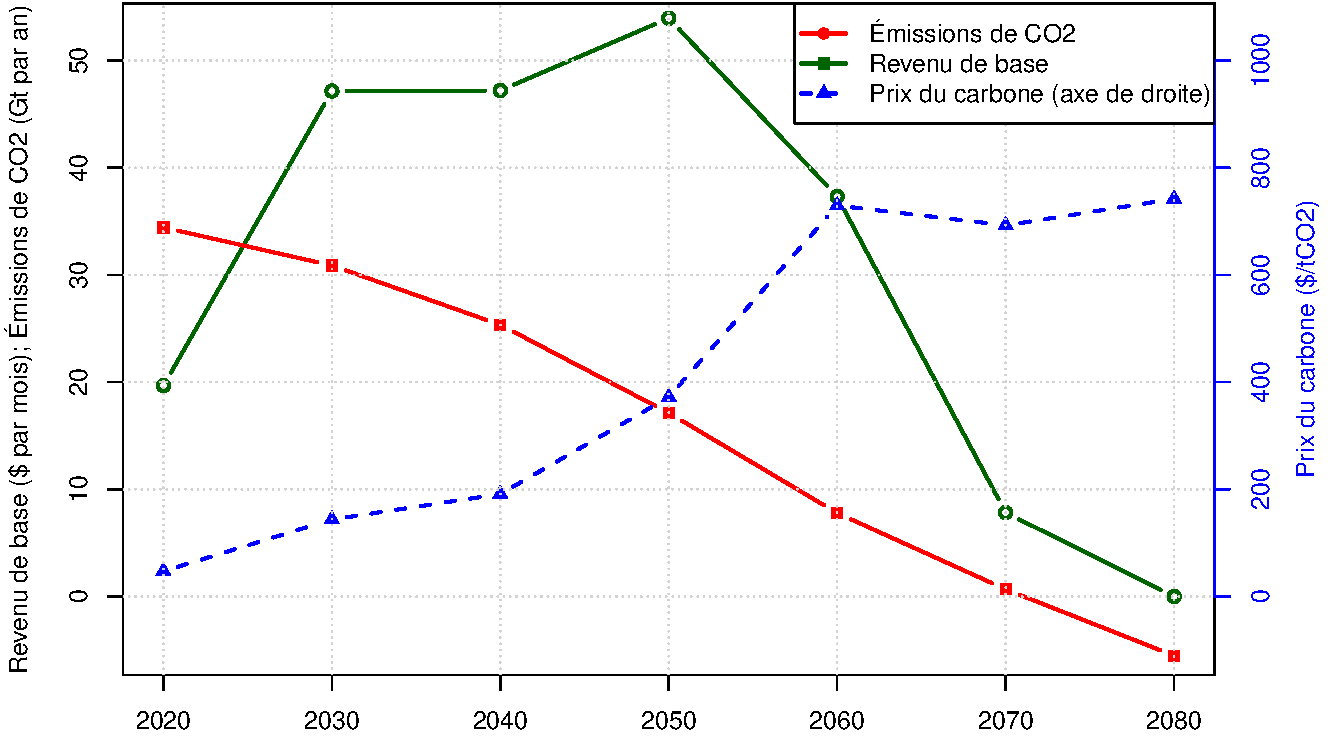
\includegraphics[width=\textwidth]{../figures/policies/GCP_trajectoires.pdf}} 
\end{figure} 

Comparé aux usages alternatifs des recettes, le revenu de base a l'avantage d'atteindre les plus pauvres et de ne délaisser personne. En outre, il permet de s'adapter au mieux aux besoins des individus, qui décideront eux-mêmes comment utiliser l'argent en fonction de leurs besoins (nourriture, soins, équipement\dots{}). 
Bien que la distribution d'un revenu de base à chaque être humain soit techniquement difficile, différentes options sont disponibles %~: soit les outils administratifs existants, soit des smartphones potentiellement connectés à l'internet par satellite
(cf. section \ref{sec:implementation}). Si les infrastructures ne sont pas prêtes à temps pour cette distribution ou si des communautés préfèrent recevoir la somme sous une autre forme, l'argent pourrait être versé aux autorités locales ou nationales afin qu'elles développent les services publics, la protection sociale et les infrastructures. 

\section{3$^\text{e}$ principe~: Un club climatique}

Le Plan serait lancé par un club de pays volontaires et mis en œuvre dès que 60~\% des émissions mondiales de CO$_\text{2}$ seraient couvertes par les entités participantes\footnote{Notons que des entités infranationales pourraient rejoindre le club même si le niveau fédéral ne le fait pas.}. Ce seuil peut être atteint par l'union de la Chine (30~\% des émissions mondiales), des États-Unis (15~\%), de l'Inde (7~\%), de l'UE et du Royaume-Uni (9~\%). Si les États-Unis ne participent pas, ce seuil serait quand même atteint dans un scénario \textit{prudent} où le club serait formé par l'UE, les pays qui bénéficieraient financièrement du Plan (19~\%, dont l'Inde) et ceux qui ne seraient ni gagnants ni perdants financièrement (36~\%, dont la Chine). % PTET expliquer plus
Dans un scénario \textit{optimiste} où l'on ajoute à cela les autres États susceptibles de rejoindre le club
\footnote{En plus des pays qui ne seraient pas perdants financièrement et de l'UE, on peut espérer une participation des États suivants~: Japon, Corée du Sud, Canada, Royaume-Uni, Norvège, Suisse, Nouvelle-Zélande, ainsi que les 12 États états-uniens où le parti démocrate a remporté les dernières élections avec plus de 10 points d'écart (en particulier la côte Ouest, l'Illinois et le Nord-Est à l'exception de la Pennsylvanie).}, 
93~\% de la population et 74~\% des émissions mondiales seraient couvertes (cf. Tableau \ref{tab:scenarios_table_fr}). 

\begin{table}[h]

\caption[Différents scénarios de club climatique]{\label{tab:scenarios_table_fr}Principales caractéristiques des différents scénarios de club climatique.}
\makebox[\textwidth][c]{
\begin{tabular}[t]{ccccc}
\toprule
\makecell{Scenario\\de club} & \makecell{Émissions\\mondiales\\couvertes} & \makecell{Population\\mondiale\\couverte} & \makecell{Revenu de base\\en 2040\\(\$/mois)} & \makecell{Contribution de l'UE\\en 2040\\(fraction de son PIB)}\\
\midrule
Tous les pays & 100\% & 100\% & 47 & 0.8\%\\
Tous sauf OPEP+ & 90\% & 97\% & 41 & 0.9\%\\
Optimiste & 74\% & 93\% & 32 & 1.1\%\\
Central & 67\% & 90\% & 25 & 1.1\%\\
Prudent & 63\% & 88\% & 22 & 1.2\%\\
UE + Afrique & 12\% & 24\% & 29 & 1.1\%\\
\bottomrule
\end{tabular}}
\end{table} % PTET? étoffer

Pour éviter le déplacement d'émissions vers des pays à la législation moins contraignante, les importations vers le 
club seraient taxées en proportion de leur contenu carbone~: c'est la tarification carbone aux frontières (que l'UE met en place à son échelle). 

\section{4$^\text{e}$ principe~: Des mécanismes de participation}

Sans aménagement supplémentaire, le Plan aurait pour effet de rendre contributeurs nets certains pays dont l'empreinte carbone est supérieure à la moyenne mondiale même si leur population est loin d'être riche. Pour tenir compte de la capacité à payer limitée de ces populations, une clause (dite d'\textit{opt out}) éviterait à des pays aux revenus intermédiaires d'être contributeur net. Ainsi, une clause dérogatoire à la mutualisation des recettes permettrait à des pays dont le PIB par habitant n'excède pas la moyenne mondiale de plus de 50~\% (comme la Chine, l'Afrique du Sud ou l'Algérie) de conserver les recettes prélevées sur leur territoire. Ces pays feraient face aux mêmes contraintes de décarbonation que les autres, mais ne seraient ni gagnant, ni perdant par rapport à une tarification carbone sans transferts internationaux. 

Le traité permettrait également à des États tels que la Californie ou l'État de New York de rejoindre le club indépendamment du niveau fédéral. En particulier, ces États seraient exemptés de tarification aux frontières, car ils ne peuvent pas mettre en place des droits de douane vis-à-vis d'autres États états-uniens. 
Ces mécanismes sont détaillés dans l'annexe \ref{ch:details}. 


\section{Mise en œuvre}\label{sec:implementation}
Outre le défi géopolitique, la mise en œuvre du Plan serait confrontée à deux défis techniques. 

\paragraph{Le contrôle des émissions}
Premier défi, les émissions de carbone doivent être déclarées, contrôlées et vérifiées, au moins % PTET? changer "au moins"?
pour les grandes unités industrielles telles que les mines de charbon ou les raffineries de pétrole. Cela pourrait s'avérer difficile dans les pays ne disposant pas d'une administration performante. Cependant, ce défi n'est pas spécifique au Plan, car le contrôle des émissions est un élément nécessaire à toute politique climatique réussie. En fait, le contrôle des émissions serait vraisemblablement facilité par le Plan par rapport à d'autres politiques climatiques, étant donné que le Plan fournirait des ressources aux pays à bas revenus (qu'ils pourraient utiliser pour développer leur administration) et ferait travailler les pays ensemble (de sorte que les pays expérimentés aideraient les autres). En outre, des projets états-uniens et européens permettent désormais de mesurer à l'aide de satellites les émissions d'une installation industrielle, d'une localité ou d'un pays\footnote{Cf. \cite{nassar_quantifying_2017,pan_potential_2021,shen_national_2023} et le \href{https://www.esa.int/Applications/Observing_the_Earth/Copernicus/Carbon_dioxide_monitoring_satellite_given_the_shakes}{projet CO2M de l'ESA}.}. Ces mesures sont utilisées pour contrôler la fiabilité des émissions déclarées.

\paragraph{Distribuer le revenu de base}
Second défi, le revenu de base doit être accessible à tous et résistant à la fraude (afin que personne ne reçoive le revenu de base plusieurs fois). Il est difficile d'atteindre les personnes qui n'ont pas d'état civil ou qui vivent dans des zones reculées. De même, il est difficile de vérifier l'identité des personnes et de s'assurer qu'elles ne sont pas enregistrées plusieurs fois. Cependant, il y a de bonnes raisons d'être confiant dans le fait que l'infrastructure nécessaire pour fournir un revenu de base peut être déployée dans les dix ans, car différentes solutions techniques sont disponibles. Premièrement, la plupart des pays disposent déjà de programmes sociaux destinés aux personnes isolées et procèdent à des campagnes d'enregistrement de la population%dans des registres biométriques
, notamment dans des registres électoraux. %En particulier, le programme \textit{Identification for Development} de la Banque mondiale finance des systèmes d'identification dans 57 pays
%\footnote{Cf. \cite{world_bank_state_2017,world_bank_benin-burkina-faso-togo-and-niger-second-phase--west-africa-unique-identification-for-regional-integration-and-inclusion-wuri-projectpdf_2020,world_bank_identification_2022}.}, dans le but de <<~garantir à tous une identité juridique~>> conformément à l'Objectif de développement durable n\textdegree{} 16.9. %En particulier, de nombreux pays africains procèdent régulièrement à des campagnes d'enregistrements de la population dans des registres électoraux biométriques. 
% 100M personnes déjà identifiées grâce à MOSIP (système open-source)
% Discussion of unified civil registry in Africa: https://www.biometricupdate.com/202306/the-case-for-an-integrated-digital-crvs-system-for-african-countries
Deuxièmement, les smartphones peuvent désormais être utilisés comme moyen de paiement et pour l'identification biométrique (et le coût d'un smartphone serait couvert par seulement quelques mois de revenu de base). %Ainsi, pour compenser les pertes de revenus des travailleurs informels lors de la pandémie de COVID, le Togo a mis sur pied en moins de deux semaines un transfert monétaire sur mobile à destination d'un million de personnes dans les zones confinées\footnote{Cf. \cite{ipa_togos_2021}}. 
Troisièmement, %alors que de nombreux endroits n'ont toujours pas accès à internet, 
l'internet par satellite offre une solution abordable pour accéder à internet depuis n'importe où. En pratique, le revenu de base des habitants d'un village suffirait à couvrir l'abonnement Starlink (de 23~\euro{} par mois au Nigeria) ainsi que l'équipement (320~\euro{})\footnote{Cf. \href{https://starlinkinsider.com/starlink-price/}{starlinkinsider.com/starlink-price}.}. %progresse rapidement et pourrait bientôt devenir bon marché et omniprésent \citep{hanson_satellite_2016}. 
%Quatrièmement, des leçons peuvent être tirées de l'expérience du système Aadhaar, lancé en 2009, qui a fourni un identifiant biométrique unique à 99~\% de la population adulte indienne en seulement 8 ans\footnote{cf. \href{https://www.thehindu.com/business/Aadhaar-covers-99-of-adults-in-India-Prasad/article17104609.ece}{thehindu.com/business/Aadhaar-covers-99-of-adults-in-India-Prasad/article17104609.ece}% \href{https://www.hindustantimes.com/india-news/over-100-crore-aadhaar-cards-issued-in-india-so-far-says-uidai-ceo-101639645906181.html}{hindustantimes.com/india-news/over-100-crore-aadhaar-cards-issued-in-india-so-far-says-uidai-ceo-101639645906181.html}
% }. %Aadhaar est lié aux comptes bancaires et utilisé pour distribuer des prestations sociales. Quand les projets en Afrique coûte en général entre 5 et 10~\euro{} par personne enregistrée, Aadhaar n'a coûté que 1\euro{} par personne\footnote{Cf. \cite{world_bank_state_2017}}. 

% L'IRIS est la techno avec le moindre taux de non-détection (0,2%) https://pages.nist.gov/IREX10/
% Pour les images de visage, c'est ~0.3% en condition réelle https://pages.nist.gov/frvt/html/frvt11.html (border border) et ~5 en 1:N https://www.neurotechnology.com/awards-frvt-1-n.html

% PNON Expliquer à ceux qui veulent séparer climate et pauvreté : Le truc c'est que la décarbonation n'est pas juste une question de financement, mais aussi de restrictions. Il faut plafonner les émissions. Se pose alors la question de comment répartir les recettes. Autant les reverser de façon équitable. => c'est déjà ce qui est dit dans le cœur du plan en gros
\paragraph{L'avancée de l'identification}
Les progrès dans ces infrastructures sont fulgurants. Lancé en 2009, le système indien Aadhaar a fourni un identifiant biométrique unique à 99~\% de la population adulte en seulement 8 ans\footnote{Cf. \href{https://www.thehindu.com/business/Aadhaar-covers-99-of-adults-in-India-Prasad/article17104609.ece}{thehindu.com/business/Aadhaar-covers-99-of-adults-in-India-Prasad/article17104609.ece}. Plusieurs problèmes ont entaché Aadhaar \citep{dreze_aadhaar_2017}, mais on peut tirer des leçons de ces échecs pour ne pas les reproduire \citep{gelb_digital_2019,muralidharan_identity_2023}. En effet, les modalités qui fonctionnent sont désormais mieux connues. Par exemple, la meilleure pratique consiste à utiliser les protocoles open-source pour l'identification biométrique (\href{https://mosip.io/}{MOSIP}) plutôt que des logiciels propriétaires.}, pour un coût d'à peine 1~\euro{} par personne enregistrée. Ce déploiement de l'identité biométrique est désormais répliqué ailleurs. % PNON Quand les projets en Afrique coûte en général entre 5 et 10~\euro{} par personne enregistrée, Aadhaar n'a coûté que 1\euro{} par personne\footnote{Cf. \cite{world_bank_state_2017}}.
En particulier, le programme \textit{Identification for Development} de la Banque mondiale finance des systèmes d'identification dans 57 pays parmi les plus pauvres 
\footnote{Cf. \cite{world_bank_state_2017,world_bank_benin_2020,world_bank_identification_2022}.}, dans le but de <<~garantir à tous une identité juridique~>> conformément à l'Objectif de développement durable n\textdegree{}~16.9. Cette identification permet ensuite d'offrir de nombreux services, et pourrait être utilisée pour le revenu de base. En Inde, Aadhaar est lié aux comptes bancaires et déjà utilisé pour distribuer des prestations sociales. De son côté, le Togo a mis sur pied en moins de deux semaines un transfert monétaire sur mobile à destination d'un million de personnes\footnote{Cf. \cite{ipa_togos_2021}.}, pour compenser les pertes de revenus des travailleurs informels dans les zones confinées lors de la pandémie de COVID. 

Bien que le défi technique demeure, il semble pouvoir être relevé par une combinaison appropriée d'infrastructures existantes et nouvelles, adaptée aux besoins spécifiques de chaque région. 

\paragraph{Haïti comme premier test}
Pour tester la bonne mise en œuvre du revenu de base, celui-ci pourrait être expérimenté dans un pays comme Haïti. Prendre une petite île comme premier test permettrait d'éviter des mouvements de population venue depuis des pays voisins pour toucher le revenu de base\footnote{Le revenu moyen en République dominicaine est sept fois supérieur à celui d'Haïti, ce qui dissipe les craintes d'un afflux en provenance de cet unique pays frontalier.}. En outre, Haïti est non seulement un des pays les plus pauvres, mais aussi un pays où l'administration est défaillante et dépassée par des gangs armés. Si la distribution d'un revenu de base se déroule positivement même dans une telle situation, on pourra raisonnablement déduire que le revenu de base peut être généralisé. En outre, distribuer un revenu de base de 40~\euro{} par mois à tous les adultes haïtiens pendant quatre ans coûterait 17 milliards d'euros, une somme qui pourrait être financée par un seul État (voire par un consortium privé). % volontariste % PTET 40 ou 50? être cohérent
Par exemple, l'État français pourrait apporter ce financement et rembourser ainsi la dette illégitime que la France a imposée à Haïti lors de son indépendance (dette imposée pour dédommager ses colons esclavagistes)\footnote{Cf. \href{http://preferences-pol.fr/Documents/Haïti.pdf}{preferences-pol.fr/Documents/Haïti.pdf}.}.
%  Haïti. Haiti 166/192 in GDP pc PPP, 148/192 in GDP pc nominal, 135/167 in democracy index, 171/180 in corruption. 8M d'adultes en 2023 => 17G€ = 44€/mois par adulte pendant 4 ans

% 1.	Plafonner les émissions en conformité avec une trajectoire +2°C, à l'aide d'un ETS
% •	Le traité définirait un budget carbone, ensuite décliné en quotas annuels.
% •	Des permis d'émissions de CO2 seraient vendus aux enchères aux entreprises émettrices, comme dans le marché du carbone (ETS) européen.	
% •	Le prix du carbone inciterait les ménages et entreprises à se décarboner. 
% •	Il serait in fine payé par les individus en proportion de leur empreinte carbone.	

% 2.	Utiliser les recettes pour verser un revenu de base mondial et résorber la pauvreté
% •	Les recettes seraient reversées sous la forme d'un revenu de base à tous les adultes.
% •	Chaque humain recevrait ainsi environ 50€/mois.
% •	Les versements sont techniquement possibles (smartphones, internet par satellites). 

% 3.	Former un club climatique avec une tarification carbone aux frontières
% •	Le traité entrerait en vigueur dès que les entités signataires couvrent 60% des émissions mondiales (Chine : 30%, pays bénéficiaires nets : 23%, UE+UK : 9%, U.S. : 15%).
% •	Les importations vers le club seraient taxées en proportion de leur contenu carbone.

% 4.	Inclure des mécanismes qui encouragent la participation de la Chine, la Californie… 
% •	Le traité permettrait à des États de rejoindre l'accord indépendamment du niveau fédéral, notamment en les exemptant de la tarification aux frontières.
% •	Une clause d'opt out de la mutualisation des recettes permettrait à des pays (comme la Chine, l'Afrique du Sud ou l'Algérie) dont le PIB par habitant n'excède pas la moyenne mondiale de plus de 50% de conserver les recettes prélevées sur leur territoire, leur évitant d'être contributeur net malgré leur empreinte carbone supérieure à la moyenne.

% 5.	Complémenter ce Plan par d'autres mesures pour le climat et la justice sociale
% •	Une fiscalité plus progressive pour compenser les classes moyennes des pays riches.
% •	Un ISF mondial finançant les pays pauvres pour traiter les responsabilités historiques.
% •	Des mesures climatiques nationales pour faciliter la décarbonation.


\chapter{Un transfert important vers les pays du Sud\label{ch:effets_distributifs}}
% Le plan mondial pour le climat : les effets distributifs dans le monde (évolution de la distrib mondiale des revenus + % de gagnants par pays + carte des pays gagnants et perdants)

On l'a vu au Chapitre \ref{ch:coeur}, le Plan mondial pour le climat opérerait une redistribution des personnes ayant une empreinte carbone plus élevée que la moyenne mondiale vers celles ayant une empreinte carbone plus faible. Dans ce chapitre, je présente des estimations des effets du Plan sur la répartition mondiale des niveaux de vie, la part de personnes gagnant financièrement suite au Plan dans chaque pays, ainsi que des cartes des gains et pertes par pays. Les méthodologies employées sont expliquée à l'Annexe \ref{ch:methodo}.

\section{La fin de l'extrême pauvreté}\label{sec:fin_pauvrete}

71~\% des humains seraient financièrement gagnants suite au Plan mondial pour le climat. Le Plan impliquerait une redistribution de 1,3~\% du PIB mondial des 29~\% d'humains ayant une empreinte carbone supérieure à la moyenne mondiale vers les 71~\% ayant une empreinte carbone plus faible. L'essentiel % 85%
de cette redistribution se ferait des 10~\% les plus riches vers les 50~\% les plus pauvres (Tableau \ref{tab:gcp_ineq}). 

\begin{table}[b]

\caption{\label{tab:gcp_ineq}Évolution de l'inégalité mondiale suite au Plan.}
\makebox[\textwidth][c]{
\begin{tabular}[t]{lccccc}
\toprule
  & \makecell{Étendue de\\la pauvreté\\à 7,5~\euro{}/jour\\(en \% du PIB)} & \makecell{Top 10~\%\\(part en \%)} & \makecell{Bottom 50~\%\\(part en \%)} & \makecell{Gini\\(en \%)} & \makecell{D9/D1\\Ratio\\inter-décile}\\
\midrule
Avant & 2,4 & 53,0 & 8,5 & 67,5 & 53,7\\
Après & 1,7 & 51,9 & 9,6 & 65,7 & 32,0\\
\bottomrule
\end{tabular}}
\end{table}

Quand on trace la distribution mondiale des niveaux de vie, l'effet du Plan est de l'ordre de l'épaisseur du trait (Figure \ref{fig:evol_distr_a}). En effet, pour 99~\% des humains, le gain net serait contenu entre $-$200~\textit{\euro{}}/mois et 50~\textit{\euro{}}/mois (Figure \ref{fig:evol_distr_b}). La perte financière serait plus importante pour les individus plus riches, mais elle ne dépasserait quasiment jamais 2,5~\% du revenu (Figure \ref{fig:evol_distr_d}). Aussi, l'indice de Gini des niveaux de vie mondial, qui mesure l'inégalité entre 0~\% et 100~\%, ne baisserait que de 2~\%. 
Pour autant, malgré des effets contenus sur la répartition des revenus dans son ensemble, le Plan changerait la donne pour les humains les plus pauvres. Le niveau de vie ferait plus que doubler pour le milliard d'humains les plus pauvres (Figure \ref{fig:evol_distr_c}). Plus personne ne vivrait dans l'extrême pauvreté (avec moins de 2~\textit{\$} par jour). 
À l'heure actuelle, le niveau de vie du 9$^\text{è}$ décile (c'est-à-dire le minimum pour faire partie des 10~\% les plus riches) est 54 fois plus élevé que celui du 1$^\text{er}$ décile (le maximum pour faire partie des 10~\% les plus pauvres). Grâce au revenu de base du Plan, ce ratio passerait de 54 à 32. 

Outre l'éradication de l'extrême pauvreté, le Plan réduirait également la pauvreté. Définie au seuil de 7,5~\textit{\euro{}} par jour, % PNON le calculer en dollar, e.g. 7€/j => pb: ça ne baisse plus que de 24%
celle-ci baisserait de 30~\%\footnote{L'étendue de la pauvreté (ou \textit{poverty gap}) est l'écart qui sépare la population pauvre du seuil de pauvreté (ici défini à 7,5\textit{\euro{}}/jour). L'étendue de la pauvreté passerait de 2,4~\% à 1,7~\% du PIB mondial suite au Plan.}. 
Par ailleurs, plus de la moitié des humains verraient leur niveau de vie augmenter d'au moins 3~\%~; et pour un tiers, l'amélioration serait d'au moins 10~\%. 

% /!\ Données en PPP et non MER
\begin{figure}[h!]
  \caption[Effet du Plan sur la répartition mondiale des revenus]{Effet du Plan mondial sur le climat sur la répartition mondiale des niveaux de vie.}\label{fig:evol_distr}
\begin{subfigure}{.5\textwidth}
  % \caption[]{Distribution des niveaux de vie avant/après le Plan.}
  \caption[]{Distribution avant/après.}\label{fig:evol_distr_a}
  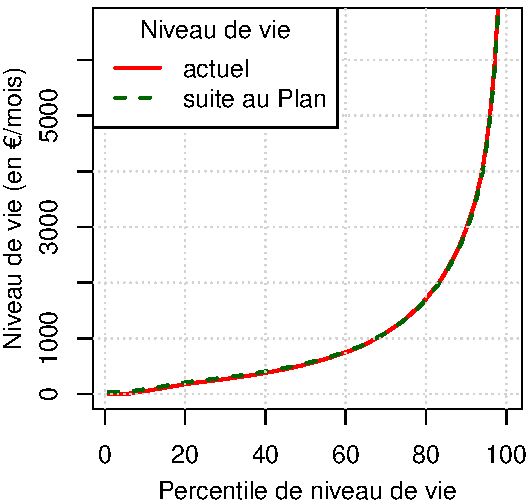
\includegraphics[width=\textwidth]{../figures/policies/gcp_rev_distr.pdf}
\end{subfigure} \quad
\begin{subfigure}{.5\textwidth}
  % \caption[]{Variation absolue de niveaux de vie}
  \caption[]{Variation absolue}\label{fig:evol_distr_b}
  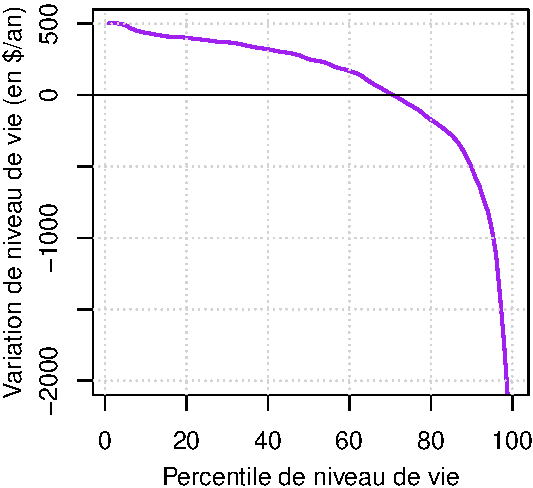
\includegraphics[width=\textwidth]{../figures/policies/gcp_diff_rev.pdf}
\end{subfigure}
\\ \quad \\
\begin{subfigure}{.5\textwidth}
  % \caption[]{Variation relative de niveaux de vie}
  \caption[]{Variation relative}\label{fig:evol_distr_c}
  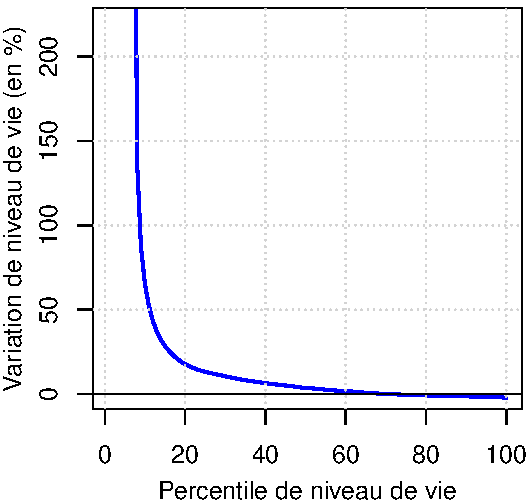
\includegraphics[width=\textwidth]{../figures/policies/gcp_var_rev.pdf}
\end{subfigure} \quad
\begin{subfigure}{.5\textwidth}
  % \caption[]{Variation relative de niveaux de vie (zoom sur les plus riches)}
  \caption[]{Variation relative (top 50~\%)}\label{fig:evol_distr_d}
  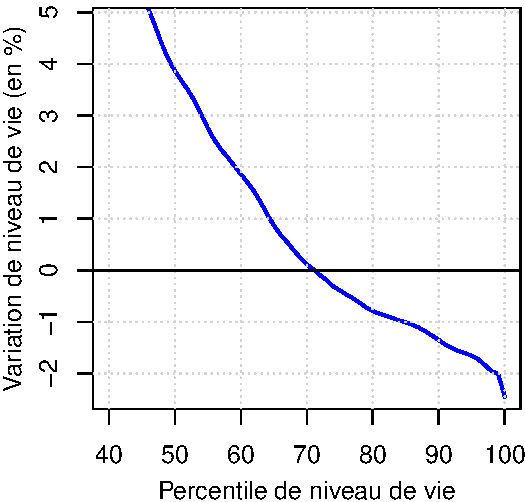
\includegraphics[width=\textwidth]{../figures/policies/gcp_var_rev_rich_only.pdf}
\end{subfigure}
{\footnotesize \textit{Note:} Calcul de l'auteur à partir d'un prix à 100 \$/tCO$_\text{2}$ et de 10~\% de réduction d'émissions, ce qui donne un revenu de base à 44~\$/mois (voir méthodologie en Annexe \ref{app:revenus}). Données~: empreinte carbone par percentile de revenus. Source~: Lucas Chancel (World Inequality Database).}
\end{figure}

\section{Une majorité de gagnants dans la plupart des pays}

Si la majorité des humains serait financièrement gagnante suite au Plan, on peut se demander quelle serait la part de gagnants dans chaque pays. La Figure \ref{fig:share_below_global_mean} présente ces chiffres, qui sont équivalents à la proportion d'individus ayant une empreinte carbone inférieure à la moyenne mondiale. En Inde par exemple, il y aurait 94~\% de gagnants, tandis qu'il n'y en aurait que 23~\% en France.  

Même si la perte financière pour le Français type serait déjà inférieure à 20~\euro{}/mois suite au Plan, le Plan devrait être complété par des mesures de redistribution nationale pour faire reposer le coût de la mue écologique sur les plus riches. Dans le Chapitre \ref{ch:premier_pas}, je montre comment une hausse de taxe sur les 1~\% ou 5~\% les plus riches permettrait de financer un transfert qui compenserait le Français ou l'États-unien type, de sorte qu'il ne perde pas financièrement. Étant donné la latitude de chaque pays pour répartir les coûts du Plan au sein de sa population, la part des gagnants par pays est finalement une information moins pertinente que la répartition des gains et des pertes entre pays, présentée ci-après.


% Pays gagnants/perdants dans différents scénarios
\section{Une redistribution Nord--Sud}

Sans surprise, le Plan mondial pour le climat opérerait une redistribution des pays du Nord vers les pays du Sud. Les principaux contributeurs seraient l'Amérique du Nord et des pays de la péninsule arabique, et les principaux bénéficiaires l'Afrique subsaharienne et l'Asie du Sud. On peut voir les effets du Plan pays par pays sur les Figures \ref{fig:gain_2030} (pour 2030) et \ref{fig:gain_npv} (pour les effets agrégés sur l'ensemble du siècle). On y voit notamment que, grâce au mécanisme de participation évoqué au Chapitre \ref{ch:principes}, des pays à revenus intermédiaires comme la Chine ne sont ni gagnant ni perdant monétairement, par rapport à la situation de référence où la décarbonation s'effectue au même rythme mais sans transferts internationaux. 

Évidemment, certains pays perdants comme l'Arabie Saoudite ou la Russie ne rejoindraient probablement pas le club climatique. J'ai également simulé les effets distributifs du Plan dans différents scénarios où la participation ne serait pas universelle. Les Figures \ref{fig:gain_optimist} et \ref{fig:gain_central} présentent les effets du Plan respectivement dans un scénario de participation \textit{optimiste} et dans un scénario \textit{central}. Comme le montre le Tableau \ref{tab:scenarios_table_fr}, même dans un scénario \textit{prudent} (où le club comprendrait uniquement l'UE et les pays non-perdants), 63~\% des émissions mondiales seraient couvertes. Les émissions couvertes monteraient à 74~\% dans un scénario optimiste où la plupart des pays à hauts revenus rejoindraient l'accord. Si ce chiffre peut sembler insuffisant pour un scénario censé être optimiste, notons toutefois que ce scénario est avant tout réaliste, puisqu'il suppose que les États-Unis resteraient hors du club climatique, même si les États états-uniens structurellement démocrates le rejoindraient\footnote{Les États structurellement démocrates sont ceux où le parti démocrate a gagné l'élection présidentielle de 2020 avec plus de 10 points d'écart.}. Gageons que ces scénarios à participation partielle ne seront valables que dans le court terme, et que le Plan réunira une masse critique de pays, suffisante pour instaurer une norme sociale mondiale en faveur du club climatique, qui poussera l'ensemble des pays à le rejoindre sur le long terme.


\begin{figure}[h]
  \caption[Parts de gagnants par pays]{Parts de gagnants suite au Plan, par pays.}\label{fig:share_below_global_mean}
  \centerline{
    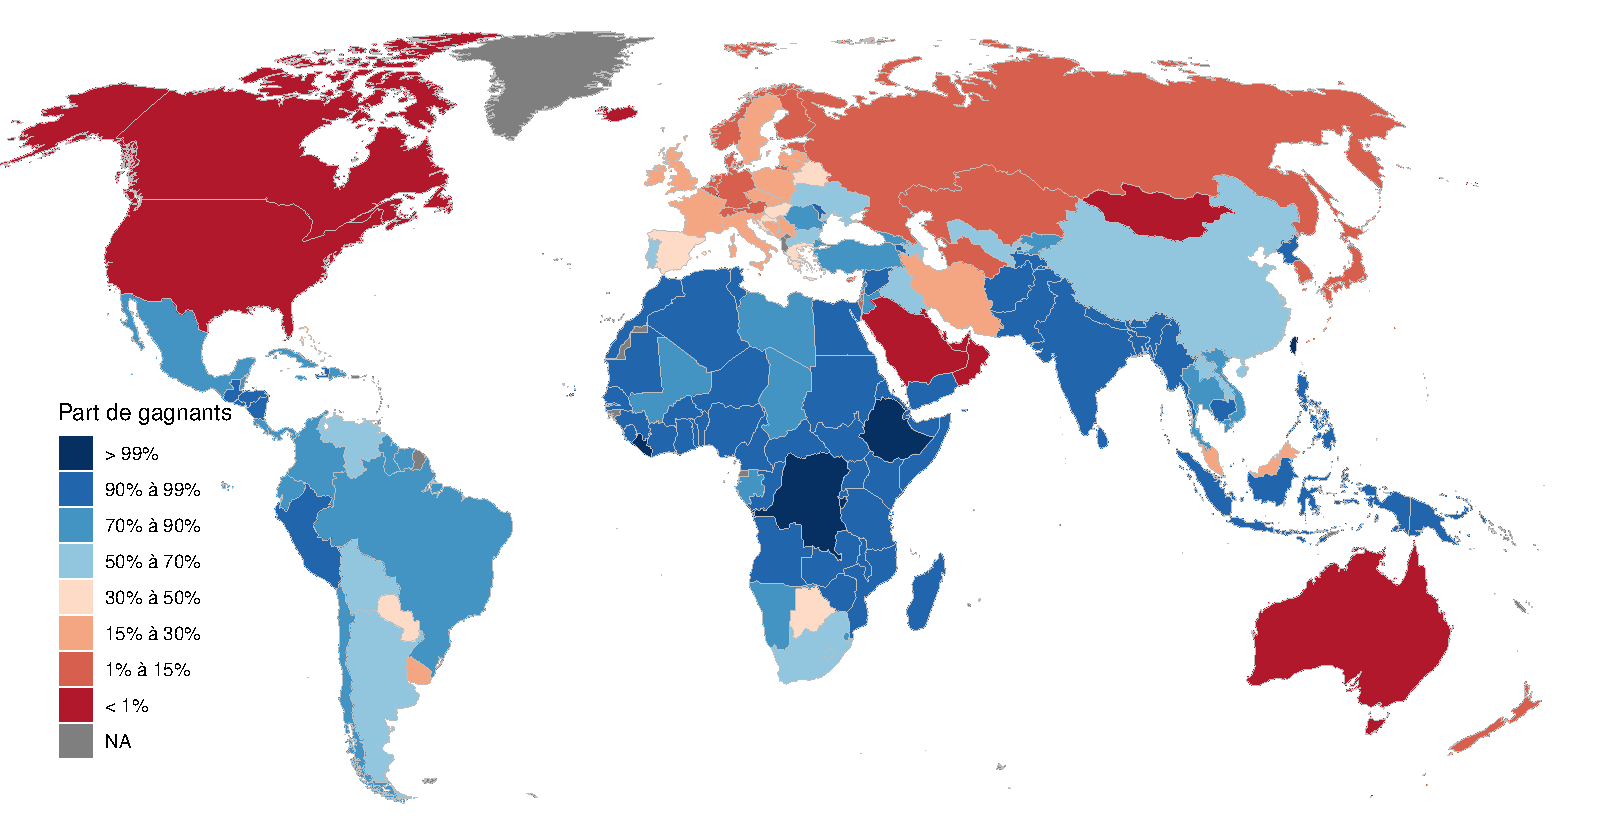
\includegraphics[width=.8\paperwidth]{../figures/maps/share_below_global_mean.pdf}
    } 
  {\footnotesize \textit{Note:} Est considéré gagnant tout individu dont l'empreinte carbone est inférieure à la moyenne mondiale. Source~: \href{http://wid.world}{wid.world}.}
\end{figure}
\begin{figure}[h]
  \caption[Gains nets par pays en 2030]{Gains ou pertes monétaires par pays suite au Plan mondial pour le climat, en 2030.}\label{fig:gain_2030}
  \centerline{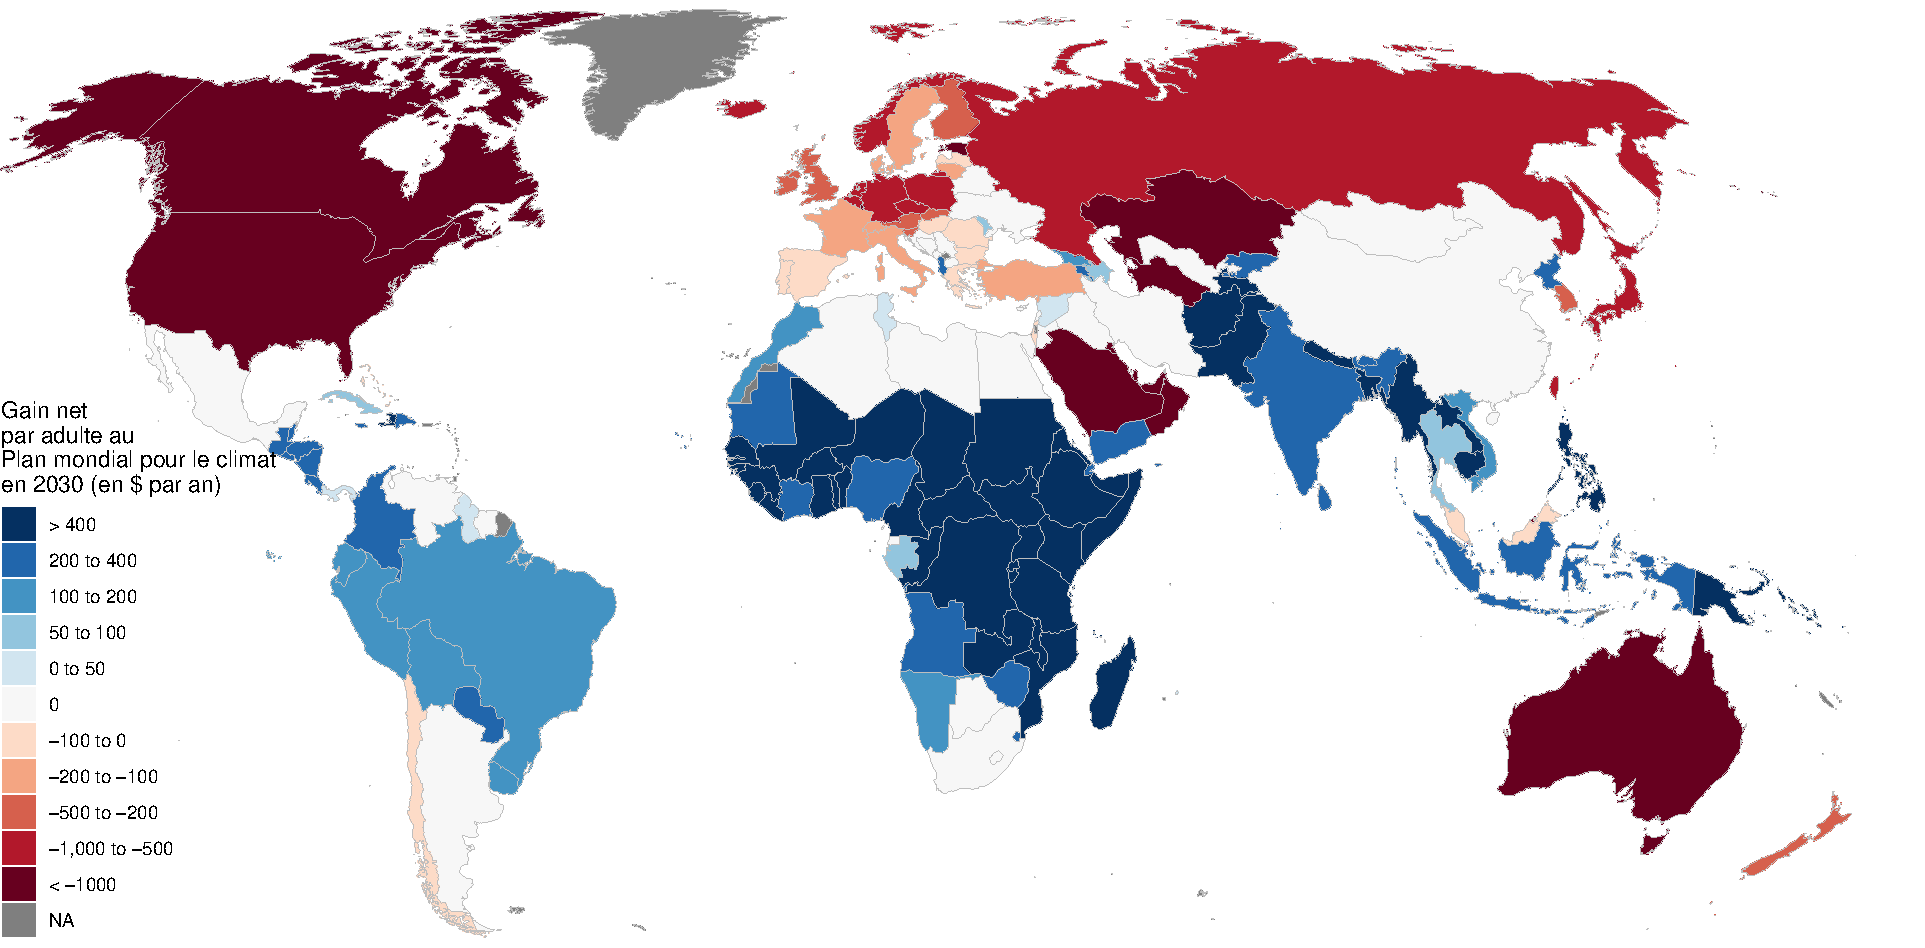
\includegraphics[width=.8\paperwidth]{../figures/maps/gain_adj_2030_fr.pdf}} % mean_gain_over_gdp_2019 mean_gain_2030
\end{figure}

\begin{sidewaysfigure}
  \caption[Gains nets par pays sur le XXI$^\text{e}$ siècle]{Gains ou pertes monétaires suite au Plan mondial pour le climat sur le XXI$^\text{e}$ siècle.}\label{fig:gain_npv}
  \centerline{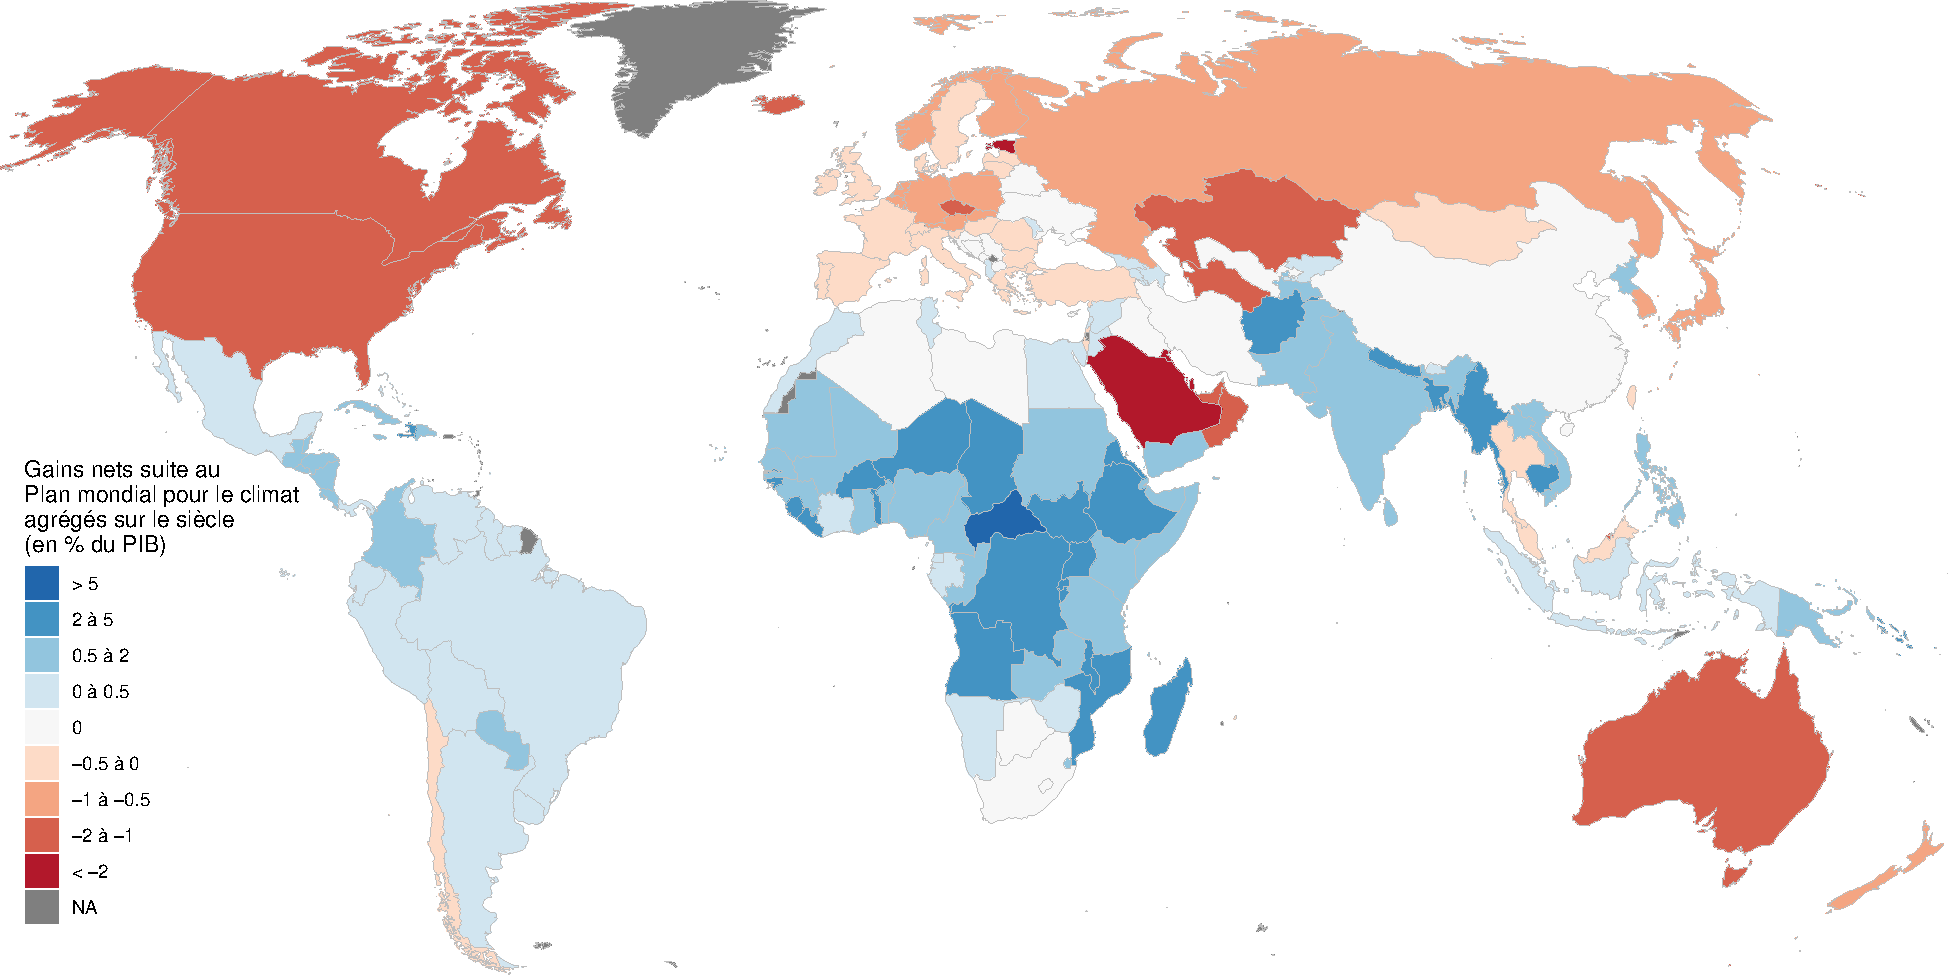
\includegraphics[width=.9\paperheight]{../figures/maps/npv_over_gdp_gcs_adj_fr.pdf}
    } % mean_gain_over_gdp_2019
  {\footnotesize \textit{Note:} La valeur nette actualisée est calculée avec un taux d'actualisation de 3~\% sur la période 2030--2100.}
\end{sidewaysfigure}

\begin{figure}[h!]
  \caption[Gains nets dans un scénario de participation \textit{Optimiste}]{Gains ou pertes monétaires par pays suite au Plan dans un scénario de participation \textit{Optimiste}.}\label{fig:gain_optimist}
  \centerline{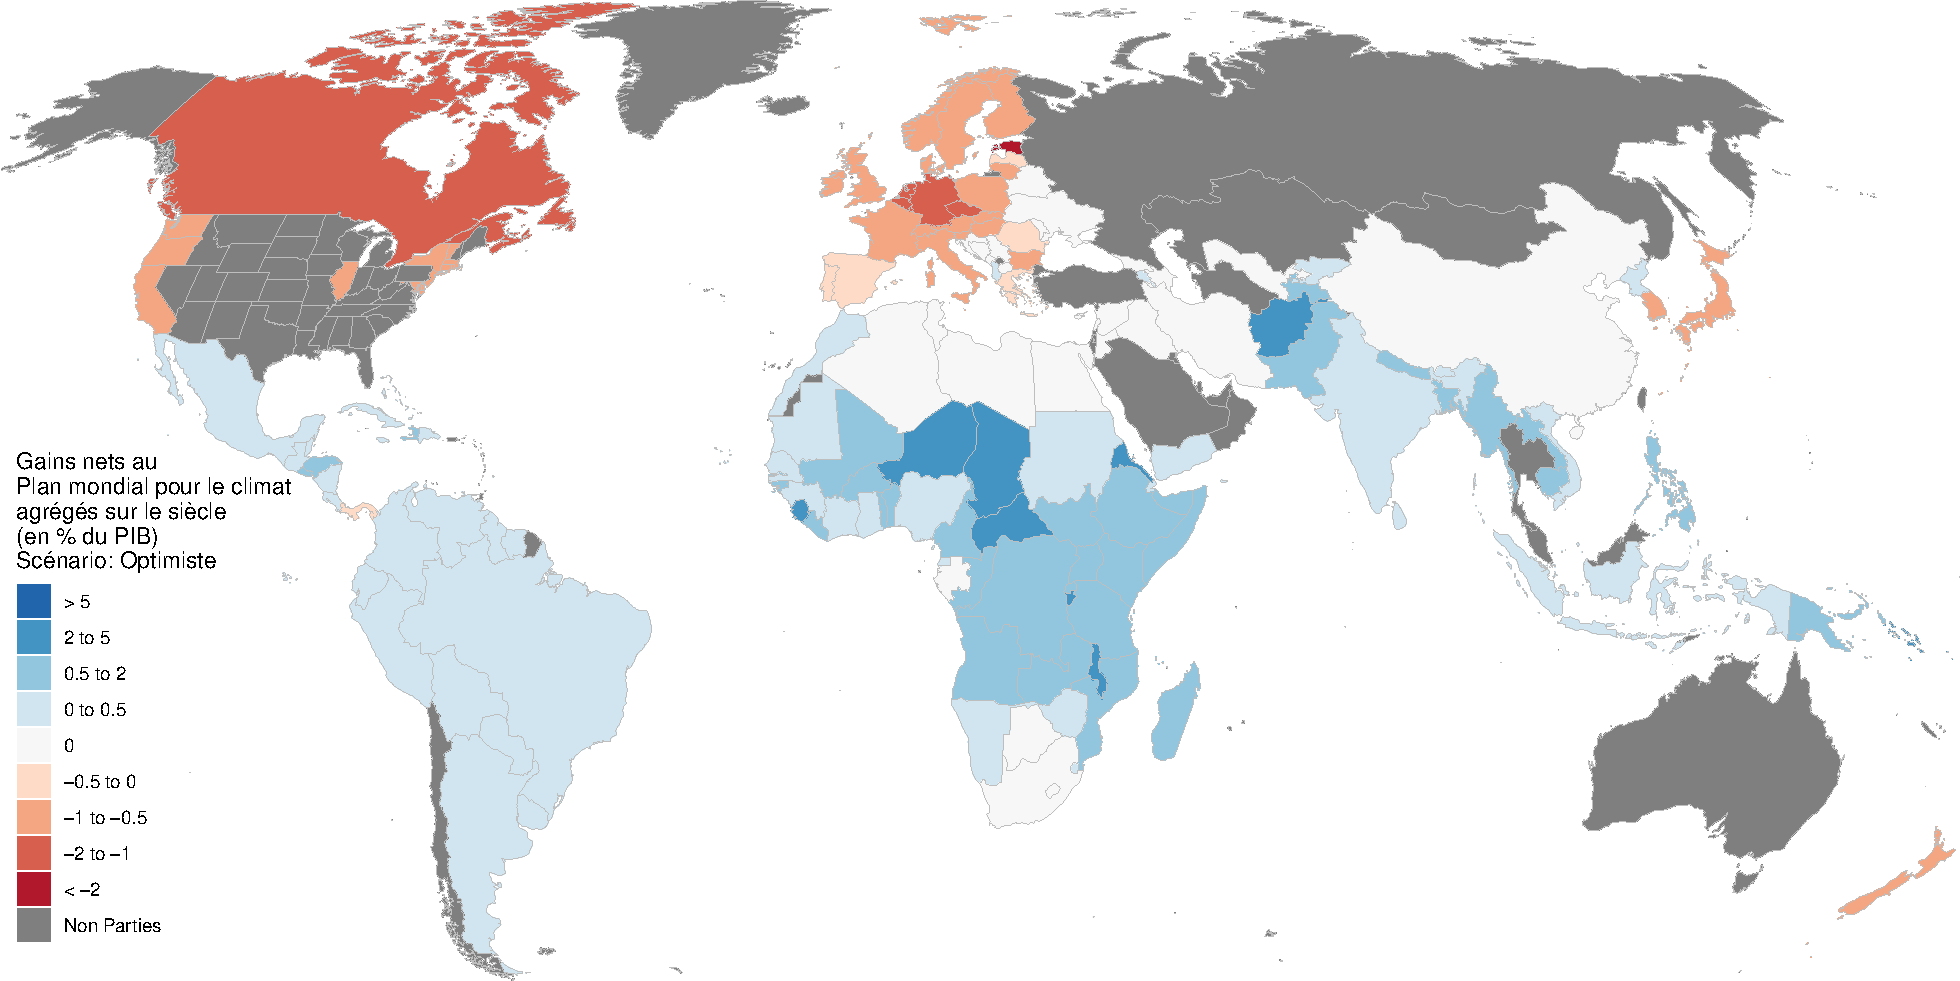
\includegraphics[width=.85\paperwidth]{../figures/maps/Soptimistic_npv_over_gdp_gcs_adj_fr.pdf}} 
\end{figure}
\begin{figure}[b!]
  \caption[Gains nets dans un scénario de participation \textit{Central}]{Gains ou pertes monétaires par pays suite au Plan dans un scénario de participation \textit{Central}.}\label{fig:gain_central}
  \centerline{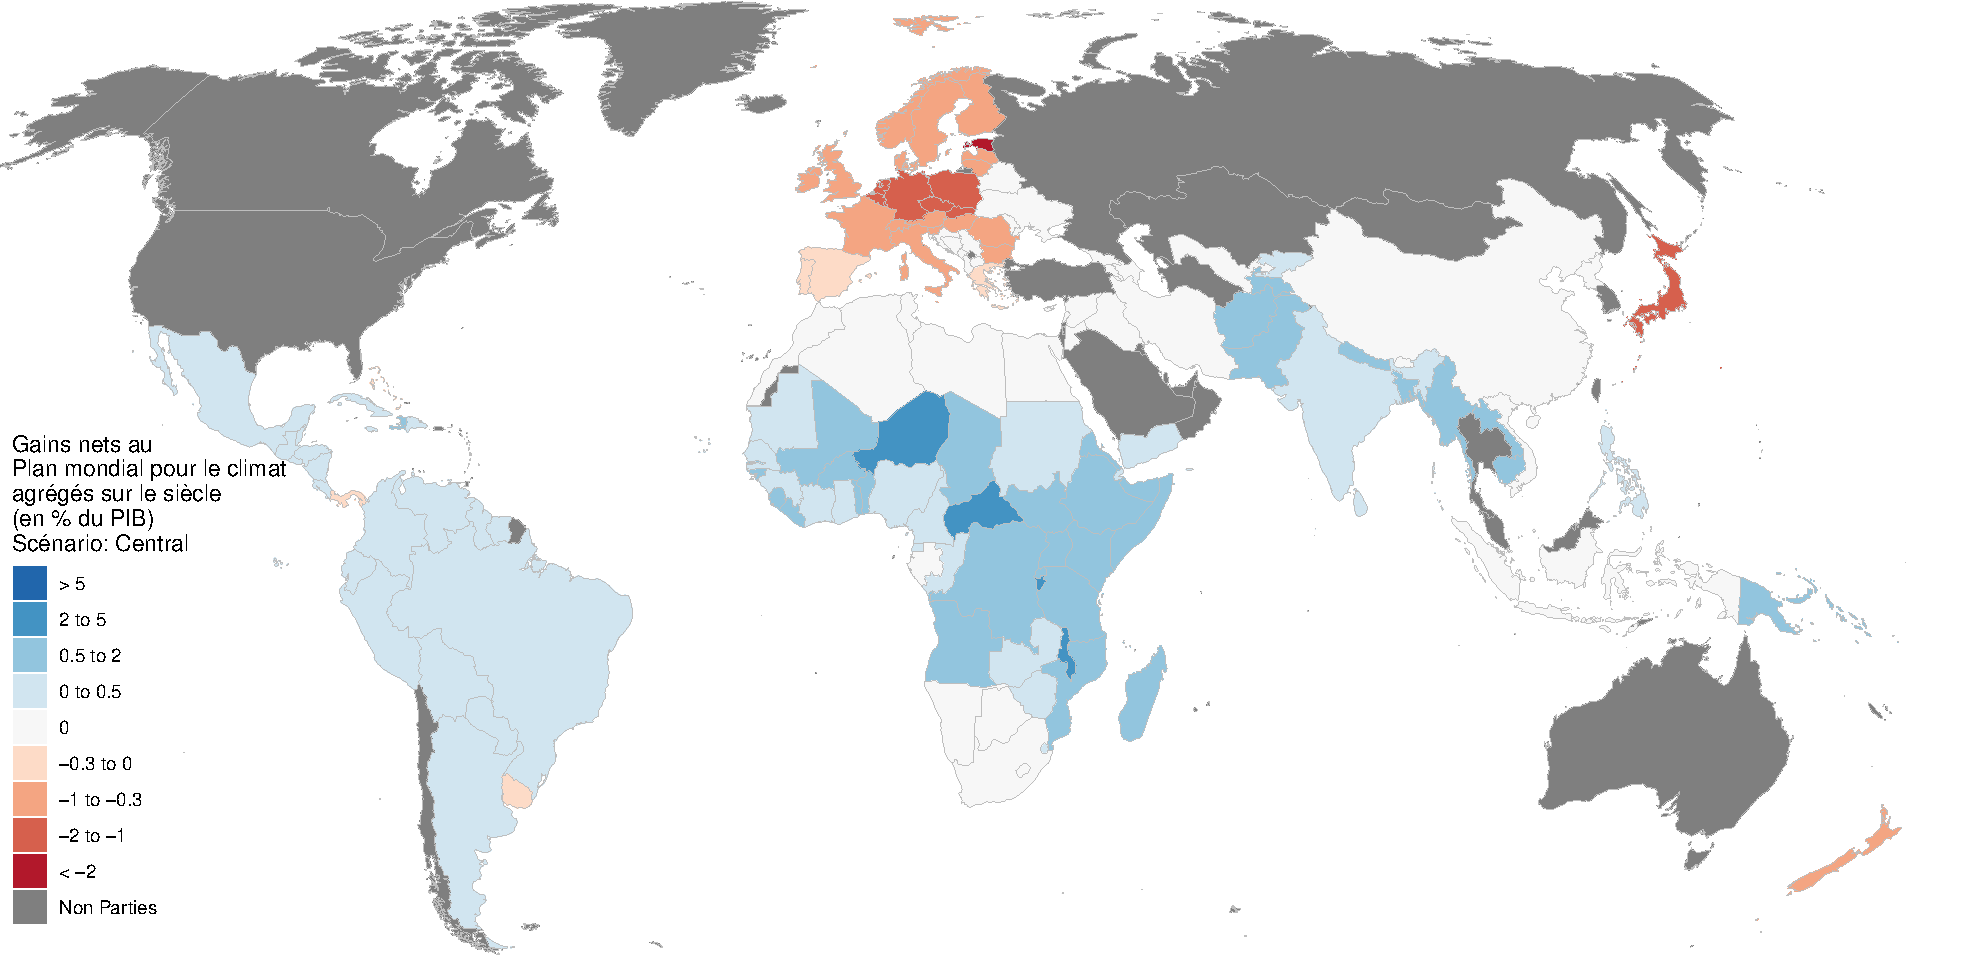
\includegraphics[width=.85\paperwidth]{../figures/maps/Scentral_npv_over_gdp_gcs_adj_fr.pdf}
    } 
\end{figure}
% \begin{figure}[b!]
%   \caption[]{Gains ou pertes monétaires suite au Plan mondial pour le climat sur le XXI$^\text{e}$ siècle}\label{fig:median_gain_adj}
%   \centerline{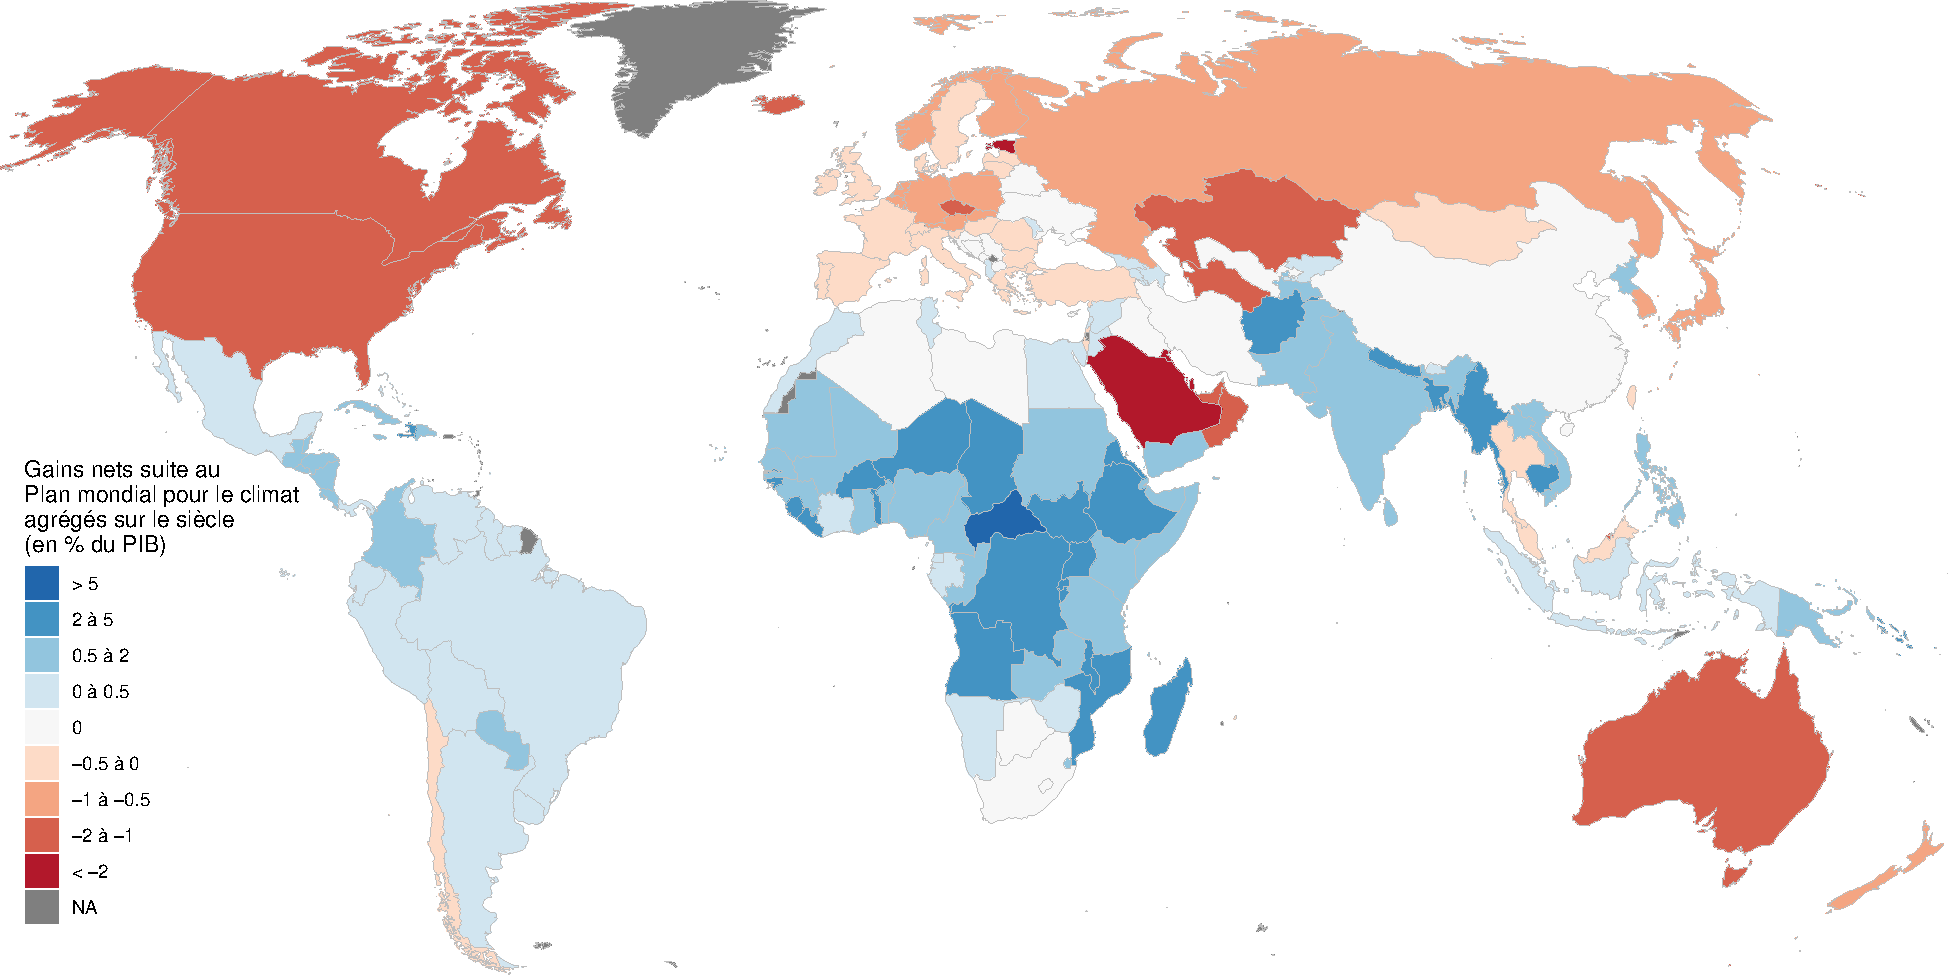
\includegraphics[width=.84\paperwidth]{../figures/maps/npv_over_gdp_gcs_adj_fr.pdf}
%     } % mean_gain_over_gdp_2019
%   {\footnotesize \textit{Note:} La valeur nette actualisée est calculée avec un taux d'actualisation de 4\% sur la période 2020--2100.}
% \end{figure}

\chapter*{\textit{Les effets concrets du Plan sur la vie des gens}}\label{ch:narr_bilan}
\addcontentsline{toc}{chapter}{\nameref{ch:narr_bilan}} 

Sept ans après l'entrée en vigueur du Plan mondial pour le climat, les trois quarts des centrales à charbon indiennes sont à l'arrêt. D'abord, le charbon est désormais plus cher que le gaz, puisqu'il contient deux fois plus de CO$_\text{2}$. Ainsi, il devient moins cher de produire de l'électricité à partir des centrales à gaz. Surtout, l'électricité d'origine renouvelable est encore moins chère, et elle se développe à toute vitesse. En effet, en prévision du Plan, le gouvernement indien a investi massivement dans le déploiement de l'éolien et du photovoltaïque. La part d'électricité d'origine renouvelable est ainsi passée de 20~\% à 80~\% en seulement sept ans. Résultat, les émissions indiennes ont baissé de 30~\% sur la période, et la pollution atmosphérique s'est nettement réduite. 

Rajesh est chauffeur de taxi à Calcutta. Il a fait le calcul, une voiture électrique coûte désormais le même prix qu'une voiture thermique, quand on tient compte du prix du carburant. Les bornes de recharge se sont largement développées dans la ville, et le prix de l'essence va continuer à monter. Rajesh est décidé~: à la prochaine panne, il se débarrassera de son vieux taxi et investira dans une Tata électrique. Rajesh gagne environ 300~\euro{} par mois, dont 50~\euro{} de revenu de base. C'est grâce à ce revenu stable que Rajesh a pu emprunter pour acheter une voiture d'occasion. % According to a survey by the National Association of Street Vendors of India (NASVI), street food vendors in India earn an average of around 8,000 to 10,000 Indian rupees per month (approximately $100 to $135 USD) https://www.quora.com/How-much-do-street-food-vendors-earn-per-day
Avant d'être chauffeur de taxi, il vendait des samoussas dans la rue et gagnait deux fois moins, tout juste de quoi vivre dans une petite chambre. Même si ses dépenses mensuelles ont augmenté de 25~\euro{} avec l'inflation, sa femme et lui ont maintenant de quoi s'offrir un joli appartement de trois pièces, dans lequel ils viennent de s'installer avec leur nouveau né. Grâce au revenu de base, il n'a plus besoin d'envoyer de l'argent à sa famille restée à la campagne, et il peut assister chaque mois à un match de cricket de son équipe fétiche. 

Jordan, lui, est contrarié par ce Plan mondial. Il habite à Vancouver, mais sa famille et ses amis les plus proches vivent à Ottawa, où il a grandi. Or, le prix du vol aller-retour est passé de 250~\euro{} à 400~\euro{}. Pour rien au monde Jordan ne renoncerait à ses week-ends mensuels dans sa ville natale. Alors, il a dû rogner sur le reste. Jordan n'a pas renouvelé son abonnement à la salle de sport --- il se contente dorénavant de jogging et d'exercices au sol chez lui, et il a un peu baissé le thermostat de son appartement (de 23 à 21\textdegree{}C) pour faire des économies. D'après ce qu'il a lu dans les journaux, le prix d'un billet devrait monter jusqu'à 800~\euro{} dans une vingtaine d'années, lorsque les avions seront propulsés à l'hydrogène. Qu'à cela ne tienne, Jordan jure qu'il continuera à faire le trajet tout aussi fréquemment, quitte à déménager dans un quartier moins cher s'il doit dégager davantage de pouvoir d'achat. Et au diable ses collègues qui le poussent à rejoindre le mouvement d'autolimitation \textit{maximum un vol par an}, il ne cèdera pas à cette mode moralisatrice~!

Rosalie, de son côté, est tout sourire. Grâce à un système de tontine, son quartier s'est cotisé pour acheter un tracteur commun. Le travail aux champs est bien plus facile, et les horaires bien moins longs, depuis l'arrivée de l'engin. Depuis le versement du revenu de base, les chantiers n'arrêtent pas à Houndé. Les compagnies d'électricité tirent des câbles dans chaque rue, la mairie installe des latrines publiques, sans compter l'hôpital flambant neuf payé par l'État burkinabé. Sur les 50~\euro{} que Rosalie reçoit chaque mois sur son téléphone, 20~\euro{} part directement en impôts (la moitié pour la ville, l'autre moitié pour l'État), et 10~\euro{} %de plus 
dans la tontine. Sur les 20~\euro{} qui lui restent, Rosalie s'est d'abord fait plaisir~: elle a acheté un matelas, en prenant un crédit sur un an avec son mari. Elle a désormais beaucoup moins mal au dos. Et surtout, elle a toujours de quoi acheter des légumes et du riz. Maintenant, elle et sa famille mangent tous les jours à leur faim.


\chapter{Un pas vers un monde soutenable\label{ch:premier_pas}} % Une des briques d'un monde soutenable
% Un pas vers un monde soutenable (le Plan n'est pas suffisant, il doit être complémenté d'autres mesures climatiques (nationales, sectorielles), d'autres mesures de redistribution mondiale (impôt sur la fortune), et l'objectif de long terme doit être d'assurer les conditions nécessaires au bien-être à chaque humain)

Le Plan proposé n'est qu'une des briques souhaitables pour construire un monde soutenable. Ce n'est pas l'objet de ce livre que de détailler un ensemble exhaustif de mesures qui permettraient d'atteindre une société harmonieuse. Pour autant, même s'il peut être négocié indépendamment du reste, le Plan mondial pour le climat ne doit pas être pensé isolément, mais comme faisant partie d'un système de mesures qui se renforcent mutuellement. Dans ce chapitre, nous dressons un aperçu de mesures complémentaires à notre Plan, tant au niveau mondial que national. À l'échelle mondiale, le Plan devrait être complété d'une gouvernance démocratique et d'autres mesures de redistribution Nord--Sud. À l'échelle nationale, la mue écologique devrait être accompagnée d'une fiscalité plus redistributive ainsi que de politiques climatiques sectorielles. 

\section{Pour un monde réellement soutenable}

\subsection{Le besoin de redistribution supplémentaire}
Dans un pays comme le Burundi, où le PIB par \textit{adulte} est autour de 500~\$ par an et les émissions de CO$_\text{2}$ à 0,1 tonne par an, notre Plan --- et son revenu de base à 50~\$ par mois --- doublerait le revenu moyen. 
%Dans un pays comme la R.D.C., où le PIB par habitant est sous les 600~\$ par an et les émissions de CO$_\text{2}$ sous les 0,1 tonne par an, notre Plan --- et son revenu de base à 50~\$ par mois --- doublerait le revenu moyen. % On ne trouve pas ça dans les simulations car la croissance du PIB de ces pays est largement sur-estimée. 
% Ce sera certes un défi d'adapter rapidement la société à un tel afflux de ressources, mais 
% https://data.worldbank.org/indicator/NY.GDP.PCAP.KD?locations=BI-CD&most_recent_value_desc=false
Pour autant, avec un revenu moyen par habitant qui passerait autour de 50~\$ par mois --- soit 140~\textit{\$} par mois ajusté au coût de la vie\footnote{Pour rappel, nous dénotons le dollar en parité de pouvoir d'achat par le signe \textit{\$} en italique.}, 
le niveau de vie resterait insuffisant pour la plupart des Burundais. Il faudrait encore davantage de redistribution mondiale pour assurer une vie décente à chacun. 

% \subsection{L'estimation du seuil de pauvreté}
% % \paragraph{7,5~\$ par jour pour une vie décente}
% Pritchett (2016) défend un seuil de pauvreté à 10$/jour, based on averaging high-income countries’ lines
On peut considérer qu'il faut au moins 7,5~\textit{\$} par jour pour avoir une vie décente dans un pays du Sud\footnote{Il n'est pas aisé %(et peut-être pas pertinent) 
de définir un seuil monétaire correspondant au minimum requis pour avoir une vie décente. Sur la base de travaux de \cite{oneill_good_2018}, Jason \cite{hickel_is_2019} mesure dans chaque pays l'atteinte de 11 indicateurs sociaux~: espérance de vie en bonne santé d'au moins 65 ans, 2~700 kcalories par personne et par jour, scolarisation dans le second degré, accès à l'électricité, à l'assainissement, etc. Il montre que dans un pays comme le Sri Lanka, les indicateurs sociaux sont presque universellement respectés, et qu'ils pourraient l'être parfaitement à l'aide de redistribution nationale supplémentaire. On peut en déduire que le revenu moyen sri-lankais, de 250~\textit{\$} %$_\text{PPA}$ 
par mois, % From PIP y_2022
est suffisant pour assurer une vie décente dans ce pays. Par ailleurs, \cite{kikstra_decent_2021} montrent que 210~\textit{\$} par mois % 5.5/d en 11PPP = 6.85 en 17PPP, 6.85*365/12 = 208
est généralement insuffisant pour avoir une vie décente, définie selon des critères équivalents. Ainsi, le seuil monétaire permettant d'assurer les besoins fondamentaux se situe probablement entre 210 et 250~\textit{\$} par mois (en moyenne sur les pays du Sud), soit entre 6,85 et 8,25~\textit{\$} par jour. Faute d'étude académique qui calcule un tel seuil, je vais donc utiliser comme seuil de pauvreté la valeur intermédiaire de 7,5~\textit{\$} par jour.}. 
37~\% de la population mondiale vit avec moins que cela. %de 7,5~\textit{\$} par jour. 
Cela coûterait 2~\% %(au plus) 4~\% 
du PIB mondial d'éradiquer la pauvreté définie au seuil de 7,5~\textit{\$} par jour\footnote{Le taux de pauvreté a été calculé pour 2030 à partir des données de \textit{Poverty and Inequality Platform} en faisant l'hypothèse d'une croissance mondiale de 4,5~\% par an d'ici-là. L'étendue de la pauvreté en dollars a été calculée à partir de la même source et divisée par le PIB mondial à partir des données de la Banque mondiale, avec la même hypothèse de croissance.}% https://data.worldbank.org/indicator/NY.GDP.MKTP.CD?locations=1W
, en procurant à chaque personne pauvre le revenu qui la sépare de ce seuil. Ce chiffre est cohérent avec le coût des investissements nécessaires pour atteindre les Objectifs de développement durable (qui recoupent largement les indicateurs sociaux d'une vie décente), estimé autour de 2~\% du PIB mondial par l'\cite{unctad_estimating_2021}. %4~\% du PIB mondial par l'\cite{unctad_world_2023}. 
Le revenu de base financé par le Plan transfèrerait environ 1~\% du PIB mondial aux personnes pauvres\footnote{En effet, les 37~\% d'humains les plus pauvres obtiennent actuellement 4,3~\% des revenus mondiaux, et cette part passerait à 5,2~\% suite au Plan, d'après la méthodologie de l'Annexe \ref{app:revenus}.}~: % en considérant 39% i.e. 3.25G de pauvres en 2030 et un transfert de 380$/an soit 32$/mois par pauvre, le transfert serait de 1.23T$/an ~ 1% GDP2030. 32$/mois correspond à RdB à 40$ - 1t/5t d'émission par pauvre. 
il faudrait donc des recettes supplémentaires de l'ordre de 1~\% du PIB mondial pour mettre fin à la pauvreté. % L'UNCTAD chiffre en 2023, donc en 2030 ça serait moins que 4% du PIB (3.1% si le PIB croît à +3.5% sur 7 ans). 
% 4T ça correspond à un rendement de 5.3% sur 75T.

\subsection{Un impôt mondial sur la fortune} % comme mesure complémentaire}
Plusieurs mesures sont envisageables pour lever une telle somme. La plus prometteuse est sans doute l'impôt sur la fortune. Tout d'abord, l'impôt sur la fortune remplit également un autre objectif, puisqu'il peut être présenté comme un moyen de solder 
les responsabilités historiques pour le changement climatique plutôt que comme une mesure de solidarité. Il est généralement admis que les pays riches sont les responsables historiques du changement climatique. Pourtant, il peut être plus fructueux d'attribuer cette responsabilité aux \textit{personnes} riches. En effet, il semble que les personnes ayant hérité d'un patrimoine bâti grâce aux énergies fossiles profitent davantage des émissions passées que, par exemple, un Ukrainien type, né dans un pays qui polluait beaucoup par le passé mais s'est depuis appauvri\footnote{En 2022, le PIB par habitant en parité de pouvoir d'achat de l'Ukraine est de 35~\% inférieur à son niveau de 1990 (et était déjà de 21~\% inférieur en 2021), d'après la \href{https://data.worldbank.org/indicator/NY.GDP.PCAP.PP.KD?locations=UA}{Banque mondiale}.}. % https://data.worldbank.org/indicator/NY.GDP.PCAP.KD?locations=UA https://data.worldbank.org/indicator/NY.GDP.PCAP.PP.KD?locations=UA
À partir du travail de \cite{fanning_compensation_2023}, j'ai calculé que la compensation due par les pays riches au titre des émissions de la période 1990--2030 s'élève à 26~000 milliards de dollars, soit 25~\% du PIB mondial
%1960--2030 s'élève à 75~000 milliards de dollars, soit 75~\% du PIB mondial
\footnote{\cite{fanning_compensation_2023} estiment à 192~000 milliards de dollars la compensation due par les pays riches pour avoir dépassé le quota d'émissions proportionnel à leur population et correspondant à un scénario de réchauffement de 1,5\textdegree{}C. Cette estimation est obtenue en multipliant les émissions cumulées sur la période sur la période 1960--2050 (en faisant l'hypothèse d'une décarbonation rapide pour 2020--2050) % PNON remove parenthèses?
avec une trajectoire de prix du carbone sur 2020--2050 correspondant au scénario 1,5\textdegree{}C. La mise en place universelle du Plan mondial pour le climat en 2030 mettrait fin à la nécessité de compenser les émissions excédentaires à partir de cette date, puisque celles-ci seraient déjà tarifées. Ainsi, pour calculer la compensation due au titre de la période 1960--2030, on peut utiliser les émissions cumulées sur cette période et la moyenne du prix du carbone sur la période 2020--2030 (soit 135~\$/tCO$_\text{2}$) plutôt que 2020--2050 (288~\$/tCO$_\text{2}$). Cela donnerait 75~000 milliards. Cependant, on peut contester les hypothèses de \cite{fanning_compensation_2023} comme étant trop radicales~: la dangerosité du changement climatique n'a été universellement reconnue qu'en 1990, et l'objectif sur lesquels les pays se sont mis d'accord est un réchauffement de 2\textdegree{}C plutôt que de 1,5\textdegree{}C. En considérant un scénario à 2\textdegree{}C sur la période 1990--2020 (ou alternativement, en prenant les hypothèses initiales avec un prix de 45~\$/tCO$_\text{2}$), on obtient 26~000 milliards. Ces calculs peuvent être reproduits sur \href{https://github.com/bixiou/compensation-atmospheric-appropriation}{github.com/bixiou/compensation-atmospheric-appropriation}.}. 
% Je précise que la monétisation de la dette climatique se base sur la méthodologie de \cite{fanning_compensation_2023}, qui mériterait d'être améliorée.}. => non en fait elle tient (presque) la route leur méthodo, cf. Zotero
En attribuant cette dette aux multimillionnaires et en étalant son remboursement dans le futur, on retombe sur un flux des riches vers les pauvres de l'ordre de 1~\% du PIB mondial\footnote{Il est financièrement équivalent de transférer directement du capital ou de verser éternellement le rendement annuel de ce capital. En prenant un taux crédible pour le rendement du capital (4~\%), une dette de 25~\% du PIB mondial peut donc être convertie en un flux annuel de 1~\% du PIB mondial.
%   Plutôt que de transférer d'un coup un patrimoine valant 75~\% du PIB mondial, les multimillionnaires peuvent verser un flux d'intérêt équivalent. 
% En attribuant cette dette aux multimillionnaires, ceux-ci devraient s'acquitter d'intérêts sur cette dette jusqu'à ce qu'elle soit remboursée. En prenant un taux crédible pour le rendement du patrimoine (4~\%), on retombe sur un flux annuel de 3~\% du PIB mondial.
}. 
% En attribuant cette dette aux multimillionnaires, ceux-ci devraient s'acquitter d'intérêts sur cette dette jusqu'à ce qu'elle soit remboursée. 
% % En prenant un taux crédible pour le rendement du patrimoine (5,3~\%), on retombe sur un flux des riches vers les pauvres de l'ordre de 4\% du PIB mondial. 
% En prenant un taux crédible pour le rendement du patrimoine (4\%), on retombe sur un flux des riches vers les pauvres de l'ordre de 3~\% du PIB mondial. 
Hormis le traitement des responsabilités historiques du changement climatique, il y a deux autres avantages à un impôt sur la fortune. D'une part, un tel impôt n'existe que dans une poignée de pays et peut donc être mis en place pour financer des pays tiers sans empiéter sur les budgets nationaux existants. D'autre part, cet impôt a le potentiel pour collecter %sans encombre 
les importantes recettes désirées tout en épargnant le commun des mortels. % 4\% du PIB mondial
% TODO? TD élaguer en termes de chiffres et scénarios

Par exemple, la somme de 1~\% du PIB mondial pourrait être collectée par un impôt mondial qui taxerait la fortune individuelle au taux de 2~\% (par an) à partir de 5 millions%, 6~\% à partir de 100 millions et 10~\% à partir de 1 milliard d'euros
\footnote{
%Les seuils de 2, 10 et 100 millions correspondent respectivement à 25, 100 et 1~000 fois le patrimoine moyen des humains. On peut imaginer d'autres barèmes qui rapporteraient également 3~\% du PIB mondial. Par exemple, des taux marginaux de 4~\% pour la fortune au-delà de 5 millions, 8~\% au-delà de 20 millions et 10~\% au-delà de 100 millions (ici, les seuils correspondent au 0,1~\%, 0,01~\% et 0,001~\% les plus riches). Ou bien, 5~\% au-delà de 5 millions et 10~\% au-delà de 50 millions. Ou encore, un taux unique de 7~\% au-delà de 5 millions. 
Le site \href{https://wid.world/world-wealth-tax-simulator/}{wid.world/world-wealth-tax-simulator} développé par \cite{chancel_world_2022} permet de simuler le barème de son choix.}. % https://wid.world/world-wealth-tax-simulator/
%Un tel barème épargnerait le commun des mortels. 
Avec un tel barème, les 99,9~\% de personnes qui possèdent moins de 5 millions de patrimoine ne paieraient pas d'impôt, et une personne possédant 10 millions paierait 1~\% d'impôt sur sa fortune\footnote{En effet, la taxe serait de 2~\% sur sa fortune au-delà de 5 millions, soit 2~\% de 5 millions, ce qui --- rapporté à 10 millions --- correspond à 1~\% de sa fortune.}. 
%Ce n'est qu'à partir de 200 millions de patrimoine que le taux effectif d'imposition (à 4~\%) se rapprocherait du rendement attendu de la fortune, et que l'impôt pourrait réduire la fortune du contribuable.

% Par exemple, la somme de 3~\% du PIB mondial pourrait être obtenue par un impôt mondial qui taxerait la fortune individuelle au taux de 2~\% (par an) à partir de 2 millions, 5~\% à partir de 10 millions et 10~\% à partir de 100 millions d'euros
% \footnote{Les seuils de 2, 10 et 100 millions correspondent respectivement à 25, 100 et 1~000 fois le patrimoine moyen des humains. On peut imaginer d'autres barèmes qui rapporteraient également 3~\% du PIB mondial. Par exemple, des taux marginaux de 4~\% pour la fortune au-delà de 5 millions, 8~\% au-delà de 20 millions et 10~\% au-delà de 100 millions (ici, les seuils correspondent au 0,1~\%, 0,01~\% et 0,001~\% les plus riches). Ou bien, 5~\% au-delà de 5 millions et 10~\% au-delà de 50 millions. Ou encore, un taux unique de 7~\% au-delà de 5 millions. Le site \href{https://wid.world/world-wealth-tax-simulator/}{wid.world/world-wealth-tax-simulator} développé par \cite{chancel_world_2022} permet de simuler le barème de son choix.}. % https://wid.world/world-wealth-tax-simulator/
% %Un tel barème épargnerait le commun des mortels. 
% Avec un tel barème, les 99,4~\% de personnes qui ont moins de 2 millions de patrimoine ne paieraient pas d'impôt, et une personne avec 4 millions paierait 1~\% d'impôt sur sa fortune\footnote{En effet, la taxe serait de 2~\% sur sa fortune au-delà de 2 millions, soit 2~\% de 2 millions, ce qui ---rapporté à 4 millions--- correspond à 1~\% de sa fortune.}. Ce n'est qu'à partir de 35 millions de patrimoine que le taux effectif d'imposition (à 4~\%) se rapprocherait du rendement attendu de la fortune, et que l'impôt pourrait réduire la fortune du contribuable.
% Avec un tel barème, les 99,4~\% de personnes qui ont moins de 5 millions de patrimoine ne paieraient pas d'impôt, et une personne avec 7 millions paierait 2\% d'impôt sur sa fortune\footnote{En effet, la taxe serait de 7~\% sur sa fortune au-delà de 5 millions, soit 7~\% de 2 millions, ce qui ---rapporté à 7 millions--- correspond à 2\% de sa fortune.}. Ce n'est qu'à partir de 10 millions de patrimoine que le taux effectif d'imposition (à 3,5~\%) se rapprocherait du rendement attendu de la fortune, et que l'impôt pourrait réduire la fortune du contribuable. % et 97,6% de Français

% REMOVED (from Ch 2): 
% De tels transferts seraient colossaux. Mais ils pourraient être intégralement supportés par les millionnaires. En se limitant au millième d'humains les plus riches, qui ont une fortune supérieure à 5 millions d'euros, et en ne taxant que leur fortune au-delà de ce seuil, avec un taux effectif progressant de 1~\% pour une fortune de 10 millions d'euros à 10~\% pour une fortune de 100 milliards, on récolterait environ 2\% du PIB mondial, et leur fortune ne baisserait même pas (puisque la plupart des milliardaires ont des rendements supérieurs à 10~\%). 
% À l'aide d'une taxation plus progressive, qui démarrerait à 500~000 euros, avec un taux de 0,25~\% pour une fortune d'un million d'euro (soit une taxe de 2~500~\euro{} par an), et progressant jusqu'à un taux de 20~\% sur les plus grosses fortunes, les recettes pourraient atteindre 6\% du PIB mondial. Si une telle redistribution était mise en place, les classes moyennes seraient largement épargnées. Certes, des emplois seraient détruits dans le secteur du luxe, puisque les plus fortunés consommeraient un peu moins, mais d'autres secteurs seraient portés par le développement des pays du Sud et créeraient des emplois orientés vers la production de biens exportés, notamment dans l'industrie. 

% Par exemple, la somme de 4~\% du PIB mondial pourrait être obtenue par un impôt mondial qui taxerait la fortune individuelle au taux de 3~\% (par an) à partir de 2 millions de dollar, 7~\% à partir de 5 millions, et 10~\% à partir de 50 millions. % https://wid.world/world-wealth-tax-simulator/
% %Un tel barème épargnerait le commun des mortels. 

% ######  Climate debt (in T$)  ##### Adapted from Fanning & Hickel
% # Fair share     2C         1.5C  Doesn't affect emissions trajec
% #   Price*   -30   -50   -30   -50  

% # 1960-2050   61   150    78   192
% # 1960-2030   58   144   >75<  187
% # 1990-2030   26    65    41   104
% # 1992-2050                    109

% *Average price 2020-30: 135.3 vs. 2020-50: 288.5 $/tCO2
% 75T (1960-2030, 1.5°C) correspond à l'éradication de la pauvreté (3% PIB en 2030)
% 26T (1990-2030, 2°C) correspond à la moitié de la taxe de base (1% du PIB)

\subsection{Vers une redistribution plus radicale}
Un tel impôt ne serait donc pas révolutionnaire~: il n'empêcherait pas l'apparition ou le maintien de fortunes milliardaires, dont les rendements sont généralement supérieurs à 7~\%\footnote{\cite{chancel_world_2022}.}. 
Son côté modéré lui vaudrait d'être soutenu par une large majorité de la population. Pour autant, une société qui maintiendrait aussi bien des milliardaires que des gens vivant avec 7,5~\textit{\$} par jour serait loin d'être socialement juste. Pour atteindre un monde réellement soutenable, il faudrait beaucoup moins d'inégalités~: %des revenus et patrimoines beaucoup moins dispersés~: 
on peut par exemple considérer que le revenu le plus élevé devrait être limité à cinq fois le revenu minimum (une norme attribuée au tout premier <<~prix Nobel~>> d'économie, Jan Tinbergen). Ainsi, les propositions formulées dans ce livre ne constituent qu'un pas vers un monde soutenable. La route est longue --- car les infrastructures et les structures sociales ne changent pas en un jour --- mais elle en vaut la peine.  

Non seulement il faut s'engager dans cette voie, mais il faudra veiller à ne pas faire marche arrière. Or, c'est ce qui risquerait de se produire en l'absence de mesure complémentaire à notre Plan, lorsque la décarbonation touchera à sa fin. %sera sur le point d'être achevée. 
À ce moment-là, les recettes liées au prix du carbone s'effondreront. Il serait désastreux que le montant du revenu de base s'effondre avec elles. Aussi, il faudra prévoir des ressources nouvelles pour maintenir (voire augmenter) le revenu de base, 
venant d'impôts sur la fortune, les hauts revenus, ou les sociétés. 
%L'impôt sur la fortune est une possibilité. On pourrait aussi imaginer un taux minimal d'impôt sur les sociétés, prélevé au niveau mondial. 

\subsection{Les autres chantiers mondiaux à mener}
La redistribution mondiale n'est pas le seul chantier nécessaire, loin s'en faut. La démocratie mondiale en est un autre. %La souveraineté nationale ne devrait pas être érigé en principe absolu. %Si beaucoup de gens sont attachés à la souveraineté nationale, c'est selon moi une erreur. 
En effet, toute décision devrait être prise à l'échelle pertinente, en vertu du principe de subsidiarité. Ainsi, les décisions qui ont des répercussions mondiales doivent être prises à l'échelle mondiale. % PNON reformuler en "des défis qui dépassent les frontières --> être traités en conséquence"
C'est notamment le cas de décisions relatives au changement climatique, aux pandémies, à l'intelligence artificielle ou au système financier. % l'effort de décarbonation de chaque pays, des politiques sanitaires lors des pandémies, de la recherche en intelligence artificielle, ou des règles du système financier. 
La forme précise de la gouvernance mondiale reste à définir, mais elle doit être démocratique, dès lors qu'on considère les inégalités de pouvoir de décision injustes au même titre que les inégalités de richesse. % PNON élaborer?

Par ailleurs, le Plan devrait être complété par d'autres traités internationaux sur les gaz à effet de serre non couverts (tels que le méthane), sur l'usage des sols et la déforestation. 

Enfin, il faut adapter le système financier international pour le rendre plus avantageux pour les pays du Sud. En particulier, la décarbonation nécessite le développement de la \textit{finance climat}, c'est-à-dire le financement de projets bas carbone. Le financement de projets dans les pays à bas et moyens revenus est entravé par les conditions désavantageuses et risquées auxquelles ils font face~: taux d'intérêt élevés, volatilité du taux de change, insoutenabilité de la dette publique\dots{} De nombreuses propositions ont été faites, notamment par le Secrétariat général des Nations unies et le Fonds vert pour le climat\footnote{Cf. \href{https://www.un.org/sustainabledevelopment/blog/2023/04/press-release-with-clock-ticking-for-the-sdgs-un-chief-and-barbados-prime-minister-call-for-urgent-action-to-transform-broken-global-financial-system/}{Bridgetown Initiative 2.0} ou \href{https://www.greenclimate.fund/sites/default/files/document/scaling-climate-finance-context-covid-19-full-report\_0.pdf}{Scaling Climate Finance}.}~: garanties publiques sur le crédit et le marché des changes, recapitalisation des banques multilatérales de développement, annulations de dette publique, augmentation des prêts entre États et allocation de Droits de Tirage Spéciaux. Derrière ces mécanismes techniques se cachent une idée simple~: apporter les fonds et les garanties nécessaires au financement de la mue écologique. Ces mécanismes reposent souvent sur des jeux d'écriture comptable relativement indolores, qui consistent grosso modo à créer de la monnaie pour financer des projets bas carbone. Sous la pression des pays du Sud, ces initiatives progressent, mais trop lentement au regard des besoins.

% Pas assez + nécessité de pérenniser le RdB après le GCP, Justification du seuil à 7$ => Recettes nécessaires pour éradiquer pauvreté à 7$ (4% world GDP) => ISF mondial qui permettrait de le faire (3% ISF + 1% GCP).
% Meilleure justification: average GDP pc of Sri Lanka, which achieves social targets. cf. Hickel (19)
% Average world wealth (World Inequality Report, 2021): 73k€ ~ 80k$
% 1/2/3/4/5/6/10/15\% > 1/2/5/10/50/100M/1/10G => 3%
% 1/2/5/7/10\% > 1/2/10/100M/1G => 3%
% >> 2/5/10\% > 2/10/100M => 3% (25x, 100x, 1k x average wealth)
% > 4/8/10\% > 5/20/100M => 3% (top .1/.01/.001%)
% > 5/10\% > 5/50M => 3.1%
% 3/10\% > 5/20M => 3.1%
% 7\% > 5M => 2.97%
% >>> 3/7/10\% > 2/5/50M => 4.2%, i.e. taux effectif de 1.8% à 5M, 4.4% à 10M, 6.5% à 50M
% 1/3/5/10\% > 1/2/5/50M => 3.95%
% 4/6/7/8/9% > 1/20/200M/1/10G => 4.22% (tax = k yield)
% 3/4/5/6/7/8% > 500k/1/20/200M/1/10G => 4.96% (tax = k yield)
% 4/10% > 1/20M => 5.03%

\section{Pour une mue sans accroc dans chaque pays}\label{sec:mue_nationale}

Dans les pays à bas revenus, le revenu de base constituera un afflux considérable de ressources, et accroîtra largement la capacité des États à lever des impôts. À l'aide (entre autres) d'impôts progressifs sur les revenus, ces États pourraient augmenter leur budget et financer les services publics, la protection sociale, et les infrastructures. Dans ces pays, seules les personnes les plus aisées --- celles ayant une empreinte carbone supérieure à la moyenne mondiale --- seraient perdantes financièrement. 

\subsection{Une redistribution nationale} % pour accompagner la mue}
En revanche, dans les pays à hauts revenus, la plupart des individus perdraient en pouvoir d'achat en l'absence de mesure supplémentaire. Certes, les personnes plus riches perdraient davantage, car elles ont une empreinte carbone en moyenne plus élevée. Pour autant, il serait à la fois injuste et impopulaire que les classes moyennes subissent une baisse de leur niveau de vie si les personnes aisées peuvent faire face aux hausses de prix des biens carbonés simplement en puisant dans leur épargne ou en rognant sur quelques dépenses superflues. Pour éviter cette inégalité, la mue écologique doit s'accompagner d'une redistribution dans les pays à hauts revenus. La mise à contribution des plus aisés remplirait trois rôles~: la compensation des classes moyennes pour éviter qu'elles ne soient financièrement perdantes, le financement d'infrastructures bas carbone pour éviter d'en faire reposer le coût sur des groupes malchanceux (tels que les ménages chauffés au fioul), %  populations spécifiques? 
et la réduction (voire la suppression) d'activités superflues fortement émettrices qui sapent la cohésion sociale.

En Europe, une hausse modeste de la taxation des 1~\% les plus riches suffirait à compenser la personne type, car l'empreinte carbone médiane n'est pas beaucoup plus élevée que la moyenne mondiale. Ainsi, une hausse de 2 points du taux d'impôt sur les revenus individuels au-delà de 15~000~\euro{} par mois permettrait de financer un transfert de 10~\euro{} par mois à chaque Français, ce qui éviterait que le Français type ne perde en pouvoir d'achat suite au Plan. Un tel transfert pourrait être opéré grâce à une revalorisation des minima sociaux (RSA, prime d'activité...) ainsi qu'une légère baisse de l'impôt sur les revenus pour 99~\% de la population. Mais il vaudrait peut-être mieux effectuer ce transfert en nature, en finançant les services publics d'éducation et de santé. Aux États-Unis, où les empreintes carbone sont bien plus élevées, il faudrait une redistribution plus conséquente pour compenser l'États-unien type. Cette compensation nécessiterait un transfert équivalent à 85~\$ par mois à chaque États-unien, financé par une augmentation des taux d'imposition pour les 5~\% les plus riches, les ménages gagnant plus que 25~000~\$ par mois\footnote{Un tel transfert pourrait être financé en faisant passer le taux marginal d'imposition de 32~\% à 41~\% pour les revenus annuels entre 315~000 et 400~000~\$, de 35~\% à 50~\% entre 400~000 et 600~000, de 37~\% à 60~\% entre 600~000 et 2,5 millions, de 37~\% à 65~\% entre 2,5 et 5 millions, et jusqu'à 70~\% au-delà de 5 millions de dollars. Le chiffrage du barème repose sur le simulateur \href{https://taxjusticenow.org/}{taxjusticenow.org} de \cite{saez_triumph_2019}.}.

% Les taxes sur les plus riches doivent financer: 3% global GDP to LICs, compensation classes moyennes, investissements verts, baisse autres impôts (TICPE, ETS), séquestration, le revenu de base quand le prix carbone baissera
% poverty reduction: 3%
% Fuel excise + carbon pricing revenues: 0.9% GDP (world, OECD), 1.4% (France), 1.7% (Germany) 0.4% (U.S., China), 2.9% (Poland), up to 3.5% in Greece in 2021 https://stats.oecd.org/Index.aspx?DataSetCode=REVPOT
% Investissements verts puis séquestration: ~1% GDP
% Compensation classes moyennes puis revenu de base LIC (ou remplacement taxes): ~1-1.5% GDP
% Total: 6%

% TODO compute rates Table
% W/Y = 4; top 1% (>1M) share = 38% => 6% Y = 9% 1.5Y = 3* their capital income
% Approximations: global top 3% (>6k€/m) has 30% pretax share, say 24% posttax => 18% posttax with more redistr i.e. 56% additional tax rate above 6.4k$. I.e. we need to collect 8.5k$. Say existing tax is 30% on top 1% and 3%, an additional 45% tax on pretax income above 10k (equivalent to an additional 80% tax on posttax income >10k) yields 7.5k (top 1% avg inc is 27k / seuil 10.4k); additional 30% tax on 6.4-10k pretax yields 1.3k (avg inc - 6.4k for top 1, 2, 3% = 3.5k, 2.5k, 0.6k)
% Avec un plafonnement des salaires, des revenus, des augmentations des hauts salaires, et une taxation des profits, on peut plafonner le revenu à 6k€/mois et récupérer 6% du PIB mondial. Mieux que helicopter money car l'argent serait pris au top 1%. Pb: ça entraînerait une déflation et une récession comptable puisque les biens de luxe ont un taux de marge élevé, et cette marge baisserait.

% Dire: ça ne serait pas une mince affaire, il faudrait une combinaison de the above, de sorte à plafonner les revenus après taxe à 6k€/mois (top 1%) ou bien d'augmenter les taxes dès 3k€/mois (top 10%)
Les équipements décarbonés (transports en commun, rénovation thermique...) et les baisses de recettes des taxes sur l'énergie fossile (TICPE, TVA, ETS) peuvent aussi être financés par des taxes supplémentaires sur les plus riches\footnote{Outre le Plan mondial pour le climat, les autres mesures évoquées dans ce chapitre nécessitent la redirection d'environ 4~\% du PIB mondial, dont 2~\% qui pourront financer la séquestration du carbone et le revenu de base mondial une fois la décarbonation achevée. %~: % PNON: virer ligne 907
% 1~\% pour lutter contre la pauvreté mondiale et solder les responsabilités historiques des plus riches dans le changement climatique, 1~\% pour compenser les pertes de recettes fiscales liées aux énergies fossiles, 1~\% pour financer des investissements décarbonés, 1~\% pour compenser les classes moyennes (ces derniers 2~\% pourront financer la séquestration du carbone et le revenu de base mondial une fois la décarbonation achevée). 
Ce coût pourrait être entièrement supporté par les 1~\% d'humains les plus riches (ceux gagnant plus de 10~000~\euro{} par mois), qui concentrent environ 15~\% des revenus après impôts. Pour ce faire, il suffirait d'augmenter de 17 points le taux d'imposition sur les revenus au-delà de 10~000~\euro{} par mois et de rendre plus progressif l'impôt sur la fortune précédemment évoqué, en portant le taux marginal à 6~\% sur la fortune au-delà de 100 millions et à 10~\% au-delà de 1 milliard. Les recettes de l'impôt sur les revenus sont estimées d'après le revenu moyen mondial (1~420~\euro{}/mois) et le revenu moyen du top 1~\% (27~000~\euro{}/mois) donnés par le \href{https://wid.world/income-comparator/}{WID}~; et celles de l'impôt sur la fortune à partir du simulateur du \href{https://wid.world/world-wealth-tax-simulator/}{WID}.% (2*1420)/(27000-10000) = 0.17, 1420 is global average income according to WID (3*... = 0.25) 
%Les 1~\% d'humains les plus riches (ceux gagnant plus de 10~000~\euro{} par mois) concentrent environ 15~\% des revenus après impôts. Ainsi, une redistribution radicale pourrait faire reposer tout l'effort sur les 1~\% ou 3~\% au sommet. Il faudrait pour cela une combinaison d'impôts sur la fortune, les profits, les revenus, voire un plafonnement des revenus, des salaires et des augmentations des salaires élevés. Cela ne serait pas une mince affaire, et cela serait peut-être plus modéré de répartir cette hausse de taxes sur les 10~\% humains au sommet (ceux gagnant plus de 3~000~\euro{} par mois, qui concentrent la moitié des revenus).
} (cf. Tableau \ref{tab:redistr_policies}). 
% Le Tableau \ref{tab:redistr_policies} résume les mesures redistributives du chapitre
Par exemple, un barème de l'impôt sur les revenus %la fortune 
plus progressif que celui évoqué précédemment permettrait de collecter le pourcent de PIB supplémentaire nécessaire au financement de la décarbonation\footnote{Cf. \cite{aie_net_2021}.}. 

% Plan: 1% PIB mondial, top 30%, extrême pauvreté
% ISFM léger: 1% PIB mondial, 2% >5M, top 0.1%, pauvreté + resp. hist.
% IR: +2pp > 15k€, 10€-$85/m/pers, top 1-5%, compensation Plan / minimas sociaux
% Interdictions jets, yachts; plafonnement des revenus et/ou du patrimoine
% revenus de 1 à 5: ?
\begin{table}[h]
  \caption[Mesures de redistribution]{\label{tab:redistr_policies}Six mesures redistributives collectant chacune environ 1~\% du PIB mondial.}
  \makebox[\textwidth][c]{
  \begin{tabular}[t]{cccc}
  \toprule
  \makecell{Mesure} & Variante & \makecell{Usage,\\effet} & \makecell{Transferts\\Nord--Sud} \\
  \midrule
  \multicolumn{2}{c}{Plan mondial pour le climat} & \makecell{Revenu de base mondial,\\fin de l'extrême pauvreté} & $\checkmark$ \\[1em]
  \multirow{2}{*}{\makecell{Impôt\\mondial\\sur la\\fortune}} & \makecell{Taux à 2~\%\\à partir de 5~M\euro{}} & \makecell{Dépenses publiques (pays du Sud),\\fin de la pauvreté et\\remboursement de la dette climatique} & $\checkmark$ \\[0.9em]% PNON specify taux ci-dessous et inverse les usages? 
  % solde resp. historiques climat / indemnise, couvre, rembourse, solde? PNON compensation de la dette climatique
    & \makecell{Taux progressifs\\à partir de 100~M\euro{}} & \makecell{Compensation des pertes\\fiscales liées aux fossiles} & \\[1em]
  \multirow{2}{*}{\makecell{Hausse de\\l'impôt\\sur les\\revenus\\à partir de~:}} & \makecell{20~000~\euro{}/mois} & \makecell{Compensation des classes moyennes\\puis revenu de base mondial} & $\sim$ \\[0.9em]
  & \makecell{10~000~\euro{}/mois} & \makecell{Investissements verts\\puis séquestration carbone}  & $\sim$ \\[0.9em]
  & \makecell{6~000~\euro{}/mois} & \makecell{Meilleurs services publics} & \\[0.2em]
  \bottomrule\\[-0.81em]
  \end{tabular}}
  \footnotesize{Note~: $\sim$ signifie des transferts Nord--Sud seulement à la fin du siècle.}
\end{table}
% \begin{table}[h]
%   \caption[Mesures de redistribution]{\label{tab:redistr_policies}Ordres de grandeur de mesures redistributives possibles.}
%   \makebox[\textwidth][c]{
%   \begin{tabular}[t]{cccc}
%   \toprule
%   \makecell{Mesure} & Variante & \makecell{Recettes\\(part du PIB\\mondial)} & \makecell{Usage\\ou effet} \\
%   \midrule
%   \multicolum{2}{c}{\makecell{Plan mondial pour le climat}} & 1,3~\% & \makecell{Fin de l'extrême pauvreté} \\
%   \makecell{ISF mondial} & \makecell{Taux à 2~\%\\à partir de 5M\euro{}} & 1~\% & \makecell{Lutte contre la pauvreté\\Solde resp. historiques climat} \\
%   \makecell{ISF mondial} & \makecell{Taux progressifs\\à partir de 100M\euro{}} & 1~\% & \makecell{Compensation des pertes\\fiscales liées aux fossiles} \\
%   \makecell{Impôt sur les revenus} & \makecell{À partir de 20~000\euro{}/mois} & 1~\% & \makecell{} \\
%   \makecell{Impôt sur les revenus} & \makecell{À partir de 10~000\euro{}/mois} & 1~\% & \makecell{Investissements verts\\puis séquestration carbone} \\
%   \makecell{Impôt sur les revenus} & \makecell{À partir de 6~000\euro{}/mois} & 1~\% & \makecell{Meilleurs services publics} \\
%   \bottomrule
%   \end{tabular}}
% \end{table}

Enfin, dans l'optique d'une mue égalitaire de la société, certaines consommations superflues pourraient être purement et simplement interdites, telles que les yachts ou les jets privés. En fait, on pourrait même considérer qu'au-delà d'un certain revenu, la consommation est nécessairement superflue, et plafonner les revenus à ce niveau. Ce niveau pourrait être déterminé chaque année en prenant la préférence médiane d'un échantillon représentatif de citoyens. Dans une enquête représentative sur un millier de Français, une majorité s'est prononcée en faveur de l'instauration d'un revenu maximum légal, avec une valeur préférée à 100~000~\euro{} par mois en médiane\footnote{Pour calculer la médiane, les 44~\% ne souhaitant pas imposer de revenu maximum légal ont été traités comme préférant une valeur infinie. Les autres ont reporté le montant de leur choix. Une variante de la question demandait aux répondants quel serait le revenu maximum dans une société idéale~: seuls 16~\% ont répondu qu'il n'y aurait pas de limite, et la médiane était alors de 15~000~\euro{} par mois \citep{fabre_determiner_2022}.}. 

Vous l'aurez compris, je suis enclin à limiter fortement les inégalités, et convaincu que les contraintes écologiques seront mieux acceptées dans une société moins inégalitaire. Je suis également partisan d'un accord \textit{mondial} sur la taxation (voire le plafonnement) des grandes fortunes, afin d'éviter l'évasion fiscale. Pour autant, les mesures de redistribution que je viens de proposer peuvent être décidées à l'échelle nationale, suivant la sensibilité de chaque peuple, de sorte que le choix du niveau de redistribution ne complique pas l'adoption du Plan mondial pour le climat. Le Plan détermine seulement la trajectoire mondiale de décarbonation et les transferts des pollueurs vers les frugaux, et préserve la souveraineté de chaque État pour mettre en œuvre les mesures complémentaires appropriées.

\subsection{Des mesures climatiques nationales} % pour réussir la mue}

En particulier, des mesures climatiques complémentaires sont nécessaires pour différentes raisons. Premièrement, la puissance publique a la compétence d'aménager le territoire et la capacité de prendre en charge des investissements de long terme~: réseau ferroviaire, transports publics, énergies bas carbone, rénovations thermiques. Deuxièmement, pour que les choix privés (d'investissements, d'équipement, de R\&D) soient alignés avec nos valeurs et avec la décarbonation planifiée sur le long terme, l'État doit définir des normes, que ce soit pour les émissions des nouveaux véhicules, l'efficacité énergétique des nouveaux bâtiments ou l'élevage des animaux. %la protection des animaux d'élevage. 
Troisièmement, la prise en charge des dépenses de décarbonation par la collectivité permet de mieux répartir l'effort financier et de lutter contre l'inégalité dite <<~horizontale~>> que constitue la grande variation des empreintes carbone pour un même niveau de revenu. % (du simple au double, voire plus). % Pottier 20

% PNON En effet / Pour comprendre?
À cause de cette inégalité horizontale, l'application du principe pollueur-payeur à travers le prix du carbone se traduit par des disparités d'effets sur le pouvoir d'achat~: quelqu'un qui se chauffe au fioul et se rend au travail en voiture perdra bien davantage que quelqu'un qui vit dans un logement bien isolé et se déplace à vélo. 
Ces disparités horizontales ne sont pas toujours justifiées, dans la mesure où des individus sont pénalisés alors que les alternatives aux énergies fossiles sont souvent inexistantes ou inabordables, et ce à cause de choix collectifs ou passés dont ils sont peu responsables (habitat pavillonnaire, chaudière thermique...). En mutualisant des coûts de décarbonation tels que la rénovation thermique et le remplacement d'une chaudière au fioul par une pompe à chaleur, quelqu'un qui se chauffe à l'électricité dans une maison bien isolée aidera, grâce aux subventions financées par l'impôt, les personnes vivant dans une passoire thermique. 

% En outre, les subventions réduisent le coût de l'option bas carbone, et réduisent ainsi le prix du carbone à partir duquel l'option bas carbone devient profitable. Dit autrement, pour inciter les individus à rénover leur maison et remplacer leur chaudière à gaz par une pompe à chaleur, on peut soit augmenter le prix du carbone (et donc du fioul), soit subventionner les travaux. 
% Si tous les pays subventionnent ces travaux, ou plus généralement, prennent des mesures climatiques complémentaires, la demande de permis d'émissions est plus faible, et le prix du carbone également. Dans le cas extrême, si les mesures climatiques complémentaires prises dans le monde entier suffisent à ramener les émissions sous le plafond mondial, il y a davantage de permis d'émissions mis sur le marché que de demande pour ces permis, et le prix du carbone est de zéro. Dans ce cas, l'inégalité horizontale est réduite à néant, puisque les émissions ne sont pas coûteuses au niveau individuel. En revanche, il n'y a plus de transferts des pays à hauts revenus vers les pays à bas revenus. En pratique, nous ne serons pas dans cette situation extrême. Avec un prix du carbone non nul, 
Les réductions d'émissions dues à des politiques climatiques complémentaires dans certains pays 
produiront quatre effets~: une réduction de l'inégalité horizontale dans ces pays, une baisse des émissions dans ces pays, une baisse du prix du carbone mondial\footnote{Prenons un exemple pour comprendre. 
% En effet, les politiques climatiques telles que les subventions réduisent le coût de l'option bas carbone et réduisent ainsi le prix du carbone à partir duquel l'option bas carbone devient profitable. % DONE phrase qui suit plus facile à lire que le jargon qui précède => remanier
% Dit autrement, p
Pour inciter les individus à rénover leur maison et remplacer leur chaudière à gaz par une pompe à chaleur, on peut soit augmenter le prix du carbone (et donc du fioul), soit subventionner les travaux. 
Les subventions réduisent le coût des travaux et réduisent ainsi le prix du carbone à partir duquel ils deviennent profitables. 
Si de nombreux pays subventionnent ces travaux, %ou plus généralement, prennent des mesures climatiques complémentaires, 
la demande de permis d'émissions est plus faible, et le prix du carbone également. 
Une interdiction des chaudières obligerait les propriétaires qui doivent remplacer leur chaudière à utiliser une source d'énergie non fossile et ferait également baisser la demande pour les permis d'émissions, et le prix du carbone avec elle. Plus généralement, toutes les politiques climatiques complémentaires réduisent le prix du carbone.}, 
et une diminution des contributions de ces pays au reste du monde (payées à travers le prix du carbone). Grâce à ce dernier mécanisme, le Plan mondial pour le climat inciterait chaque État participant à mettre en œuvre des politiques climatiques complémentaires. 

% (according to https://thomasblanchet.github.io/wealth-tax/ for the U.S., 16% GDP short term and 3.7% long-term/ 6% long-term with lump-sum rebate)
% Blanchet (22) finds a revenue-maximizing rate of 12% above 50M in the U.S.
% For example, a progressive wealth tax with the following schedule could raise 6\% of the GWP: 0.5\% marginal tax rate between \$500,000 and \$1 million, 1\% between \$1 and \$2 million, 3\% between \$2 and \$5 million, 5\% between \$5 and \$20 million, 10\% between \$20 and \$100 million, and 20\% above \$100 million.
% => qq'un avec 5M (1M) est taxé à 102.5k/an (2.5k) soit 2% de 5M (0.25% de 1M) i.e. il lui reste 8k/mois (3k) pour vivre de ses rentes (pour un rendement de 4%)

% En outre, même si ces disparités d'effets sur le pouvoir d'achat ne font que traduire le principe pollueur–payeur pour des personnes ayant des empreintes carbone différentes, beaucoup les trouvent injustes dans la mesure où des individus sont pénalisés à cause de choix dont ils sont peu responsables, notamment des investissements décidés à une époque où les émissions de gaz à effet de serre n'entraient pas dans les critères de décision (chaudière thermique, habitat pavillonnaire, automobile...). Certes, d'ici 2040 les gens ont le temps de changer leurs modes de vie : de déménager dans un logement plus petit et plus près de leur lieu de travail, de faire des travaux d'isolation ou d'installer une pompe à chaleur. Le temps nécessaire à ces adaptations est d'ailleurs un argument pour retarder l'entrée en vigueur de la taxe, celle-ci produisant déjà des effets (par anticipation) dès lors que sa trajectoire de prix sur le long terme est définie et crédible. Mais bien souvent, des ménages se retrouvent dans une situation de dépendance vis-à-vis des énergies fossiles car les alternatives sont inexistantes ou inabordables. Les locataires n'ont pas la maîtrise sur l'isolation ou la chaudière de leur logement tandis que les banques sont frileuses pour apporter des solutions de financement aux propriétaires qui souhaiteraient payer les travaux grâce aux économies d'énergie ; les transports publics sont trop peu fréquents ou leur desserte insuffisante pour se substituer à la voiture individuelle en zones rurales et péri-urbaines ; les routes n'offrent généralement pas de piste cyclable ; etc. BOF détailler avec la dernière phrase ?

%     \bbsp \ip Lowering a country's emissions reduces what it pays to the rest of the world.
%     \ip By mutualizing some decarbonization costs, national climate policies can reduce horizontal inequalities (discrepancies in private costs between individuals with similar income but different carbon footprints).

% >> Il y a un consensus parmi les économistes du climat que la politique climatique optimale mêle différents instruments : une tarification carbone, des investissements publics (par exemple dans les transports en commun), des subventions (par ex. à la rénovation thermique), des normes (par ex. sur la construction de nouveaux bâtiments) et des interdictions (par ex. l'élevage intensif). La prise en charge par la collectivité de dépenses de décarbonation (telles que la rénovation thermique et le remplacement d'une chaudière à gaz par une pompe à chaleur) permet de répartir l'effort financier sur toute la population (quelqu'un qui se chauffe à l'électricité dans une maison bien isolée aidera, grâce aux subventions financées par l'impôt, les personnes vivant dans une passoire thermique). 
% >> Enfin, la puissance publique doit coordonner la transition en prévoyant et en orientant les choix d'infrastructures énergétiques et de transports, d'usages des sols, et en s'assurant un approvisionnement adéquat en ressources, notamment humaines. Par exemple, la planification dans un pays comme la France devrait conduire à développer massivement des formations aux techniques d'isolation des bâtiments.

% >> Aussi comme la puissance publique a la compétence de l'aménagement du territoire et qu'elle peut financer des projets de long-terme à haut rendement social même s'ils sont peu profitables et risqués à court-terme, il est souhaitable qu'elle finance des équipements à faible émissions : transports publics, rénovations thermiques, énergies renouvelables, etc. Dans la mesure où ces investissements sont financés par une mise à contribution des plus riches et bénéficient de façon disproportionnée aux plus modestes (c'est souvent le cas pour les transports publics), leur effet distributif est préférable à celui d'une taxe carbone. De tels investissements, comme toute politique d'abattement alternative, permettent de baisser le niveau de la taxe carbone requis pour obtenir une réduction d'émissions donnée. Or, leurs effets distributifs justifient souvent d'alléger ainsi la taxe carbone, car même si cela dévie de la solution minimisant les coûts, ces derniers sont répartis plus équitablement (Stiglitz, 2019). Cette même logique s'applique d'ailleurs à la surtaxation de produits disproportionnément employés par les plus riches, tels que le kérosène ou les voitures de sport. 


\chapter{L'appel pour la redistribution mondiale\label{ch:appel}}
% L'appel pour la redistribution mondiale (description de l'activité de Global Redistribution Advocates et de CASCA, lien vers la lettre ouverte aux dirigeants pour la redistribution mondiale - que nous prévoyons de publier dans les grands journaux type The Guardian, Le Monde..., appel à une manifestation mondiale en soutien à cet appel le 1er décembre 2024 lors de la COP29).

\section{Global Redistribution Advocates}

En avril 2023, deux mois après avoir pris connaissance des résultats d'enquête révélant un fort soutien aux mesures de redistribution mondiale, j'ai co-fondé une association de plaidoyer pour ces mesures avec d'autres personnes convaincues. \textit{Global Redistribution Advocates} (c'est son nom) défend les trois mesures testées dans l'enquête sur 20 pays qui obtiennent plus de 70~\% de soutien chacun des pays (cf. Figure \ref{fig:oecd}). Outre le Plan mondial pour le climat, nous défendons~: 
\begin{itemize}
  \item Un \textbf{impôt mondial sur la fortune}~: appliqué par les pays volontaires sur le patrimoine supérieur à 5 millions d'euros, la moitié de ses recettes serait allouée aux pays à bas revenus.
  \item Une \textbf{assemblée mondiale pour le climat}~: élue à la proportionnelle sur des listes mondiales, elle aurait pour rôle de rédiger un traité sur le changement climatique.
\end{itemize}

Plus généralement, Global Redistribution Advocates (GRA) a pour vocation de défendre des mesures de redistribution mondiale des richesses ou du pouvoir, qui sont soutenues par une majorité au sein des populations concernées. Pour chacune de ces mesures, nous déployons une campagne~: une note décrivant la mesure, une pétition, et du plaidoyer auprès de responsables politiques. Nous avons choisi ces trois mesures car elles couvrent trois sujets essentiels (climat, inégalités, démocratie) et qu'elles ne sont pas portées par d'autres associations. Par ailleurs, nous travaillons de concert avec différents réseaux d'associations. 

\subsection{Les associations partenaires}

Sur le climat, nous nous inscrivons dans la \textit{Cap And Share Climate Alliance} (CASCA), une coalition d'associations qui défendent un système de \textit{cap and share}, dont le Plan mondial pour le climat est une variante. \textit{Cap and share}, ça signifie \textit{plafonner} les émissions, \textit{et partager} les recettes générées par la vente de permis d'émissions de façon égalitaire entre tous les humains. C'est l'association irlandaise \textit{Feasta} (et à travers elle l'économiste Caroline Whyte) qui fut la première à militer pour un \textit{Cap and share}, dès 2005. En ce moment, c'est l'association \textit{Equal Right} (et notamment sa directrice Laura Bannister) qui est centrale dans CASCA, et a rassemblé une vingtaine d'associations (la plupart africaines) sous cette bannière. La variante du \textit{Cap and share} défendue par Equal Right est légèrement différente du Plan mondial pour le climat~: elle n'inclut pas de mécanisme de participation (ce qui entraîne que des pays à moyens revenus comme la Chine seraient perdants), et propose une planification dans l'allocation des quotas plutôt qu'une vente aux enchères suivant une logique de marché. Plus généralement, la proposition de CASCA a une tonalité plus radicale et anticapitaliste que la nôtre. Cela n'empêche pas que GRA soutienne la proposition d'Equal Right, et réciproquement. Nos différences sont en réalité complémentaires, et cela se retrouve dans nos approches du plaidoyer~: Equal Right cherche avant tout à fédérer le mouvement pour le climat derrière le \textit{Cap and share}, tandis que GRA cherche à convaincre des partis politiques et des gouvernements. 

% PTET? mettre ce paragraphe sur CAN et le compléter. Climate Action Network, the world's leading network of climate action organisations, and the global civil society lead on climate negotiations 
% Climate Action Network, le premier réseau mondial d'organisations d'action climatique, et le chef de file de la société civile mondiale pour les négociations sur le climat.
% Le mouvement pour le climat comprend une myriade d'associations, dont les plus influentes sont Greenpeace, WWF, Friends of the Earth, 350.org, Environmental Defense Fund, ou encore le Sunrise Movement. Toutes ces associations sont membres du Climate Action Network (CAN), dont le chapitre français s'appelle le Réseau Action Climat. CAN coordonne les différentes associations de son réseau, fait émerger des positions communes, et dispose d'une importante capacité de plaidoyer pour défendre ces positions. 

% PTET? enlever le paragrapher suivant?
Le mouvement fédéraliste mondial est lui aussi fédéré autour d'une organisation~: le World Federalist Movement (WFM). C'est grâce au plaidoyer du WFM qu'est née la Cour pénale internationale en 1998. Désormais, la campagne phare du WFM est l'UNPA, acronyme anglais de l'Assemblée parlementaire des Nations unies. Cette campagne propose une réforme graduelle de l'ONU dont l'aboutissement serait une assemblée élue au suffrage direct et disposant d'un pouvoir législatif contraignant. Plutôt qu'une réforme de l'ONU, d'autres associations du mouvement fédéraliste mondial s'attachent à mettre en place des assemblées tirées au sort~: la Global Assembly, qui a réuni 150 humains tirés au sort pour adopter une position commune sur le changement climatique, fut la première expérience de ce type en 2022. 
À GRA, nous soutenons ces initiatives, mais explorons une troisième voie~: 
% une assemblée élue sur des listes mondiales, avec un rôle consultatif sur le changement climatique, mise en place par les pays volontaires. 
une assemblée élue sur des listes mondiales, dans des pays volontaires, ayant pour rôle de proposer des traités sur le changement climatique. 
Son rôle serait uniquement consultatif car nous réalisons qu'une assemblée démocratique mondiale devrait d'abord faire ses preuves avant d'être dotée d'un pouvoir législatif. Pour autant, l'émergence d'un débat public mondial sur la justice climatique serait en lui-même fructueux. 

Enfin, différentes associations militent pour un système fiscal international. Alors qu'Oxfam fait campagne pour l'impôt sur la fortune (sans préciser l'usage de ses recettes), les autres associations se concentrent sur l'agenda actuel des négociations sur ces sujets~: l'ICRICT\footnote{Pour \textit{Independent Commission for the Reform of International Corporate Taxation}.} 
propose une version équitable de l'accord international sur l'imposition des sociétés, Attac s'est constitué pour défendre une taxe sur les transactions financières, tandis que Tax Justice Network lutte pour mettre fin à l'évasion fiscale à travers des échanges automatiques d'information entre autorités et la création, à terme, d'un registre mondial répertoriant tous les actifs (une sorte de cadastre étendu aux titres financiers). Bien que cela coïncide avec leurs valeurs, aucune de ces associations ne se consacre directement à la redistribution Nord--Sud. Ainsi, alors même que notre proposition d'ISF qui financerait les pays à bas revenus n'a rien de révolutionnaire, c'est la proposition la plus radicale dans ce tissu associatif. 

\subsection{La stratégie}

L'ambition de GRA est qu'une coalition internationale de partis politiques et de gouvernements fassent campagne sur une (ou plusieurs) mesures commune(s) de redistribution mondiale. Depuis notre lancement, nous avons rencontré des dizaines de responsables politiques (eurodéputé\textperiodcentered{}e\textperiodcentered{}s, conseillers ministériels, hauts fonctionnaires) de différents pays (Inde, Brésil, Colombie, Allemagne, France, Espagne, Afrique du Sud\dots). Notre proposition qui suscite le plus d'engouement est l'impôt mondial sur la fortune. En France, elle est notamment soutenue par Nicolas Sansu (PCF), Manon Aubry (la France insoumise), Sandrine Rousseau (EELV), Aurore Lalucq (Place publique), ou encore Pascal Canfin (Renaissance). L'année qui vient offre une opportunité à saisir pour changer le cours du monde~: en 2024 ont lieu les élections européennes, mais c'est aussi une année d'élections aux États-Unis, au Royaume-Uni, en Inde, en Indonésie, au Bangladesh, au Mexique, en Égypte, au Ghana\dots{} Notre espoir est que Lula profite de la présidence brésilienne du G20 pour mettre à l'agenda la redistribution mondiale. 

Pour faire naître cette coalition, nous prévoyons de publier une lettre ouverte dans des journaux à grands tirages du monde entier. Nous travaillons d'arrache-pied pour que la liste des signataires soit la plus fournie possible. Cet appel pour la redistribution mondiale reprend les propositions en ce sens formulées par le monde  associatif (y compris GRA) et par le monde politique (et en particulier les pays du Sud). Il se conclut par un appel à une manifestation mondiale, un an après sa publication. En effet, la clé du succès réside dans la pression populaire. Ci-après, je reproduis le texte de cet appel.%, purgé des notes de bas de page qui référencent les différentes propositions auxquelles le texte fait allusion. 

\section{Le texte de l'appel}
% https://docs.google.com/document/d/1KS3DjOWepXaX3MEcQi3Bufu-gwgjXAPo/edit?usp=drive_web&ouid=117941608398819077564&rtpof=true

\begin{center}
\textbf{Nous exhortons les dirigeants mondiaux à mettre en œuvre des politiques de redistribution mondiale~!}
\end{center}

Nous exhortons les dirigeants mondiaux à mettre en œuvre des politiques visant à mettre fin à la pauvreté, à stopper le réchauffement climatique et à réduire les inégalités. 

Pour atteindre le premier objectif de développement durable et mettre fin à l'extrême pauvreté d'ici 2030, des transferts internationaux sont nécessaires
\footnote{Banque mondiale (2022), \href{https://www.worldbank.org/en/news/statement/2022/10/05/world-bank-group-president-david-malpass-foreword-to-the-poverty-and-shared-prosperity-report}{World Bank Group President David Malpass: Foreword to the Poverty and Shared Prosperity 2022 Report}.}%
. Pour réussir la décarbonation dans les pays à bas revenus, des transferts internationaux sont nécessaires
\footnote{IEA (2023), \href{https://www.iea.org/reports/net-zero-roadmap-a-global-pathway-to-keep-the-15-0c-goal-in-reach/}{Net Zero Roadmap}.}%
. Pour permettre à tous les humains de mener une vie décente, des transferts internationaux sont nécessaires. 

L'écart est sidérant entre les niveaux de vie des pays à hauts revenus, où vivent 1,2 milliard de personnes, et ceux des pays à bas revenus, où vivent 700 millions de personnes\footnote{Les pays à bas revenus sont définis par la Banque mondiale comme ceux ayant un PIB par habitant % ce n'est pas en PPA
inférieur à 1~135~\$ par an. Ils sont composés de 25 pays en Afrique subsaharienne et de 4 en dehors (Afghanistan, Corée du Nord, Syrie et Yémen).}. 
Le PIB par habitant est 62 fois plus élevé dans les pays à hauts revenus que dans les pays à bas revenus
\footnote{Banque mondiale (2023), \href{https://data.worldbank.org/indicator/NY.GDP.PCAP.CD?end=2021\&locations=EU-ZG-XD-XM-1W-IN-US-CD-BI-LU-CN\&start=2021\&view=bar}{Indicateur NY.GDP.PCAP.CD}.}%
. En d'autres termes, un transfert de seulement 1~\% du PIB des pays à haut revenus vers les pays à bas revenus doublerait mécaniquement le revenu national de ces derniers. Un transfert de cette ampleur peut être financé par un impôt sur la fortune modéré, de 2~\% sur le patrimoine au-delà de 5 millions de dollars, ce qui laisserait 99,9~\% de la population non affectée
\footnote{Chancel et al. (2022), \href{https://wid.world/world-wealth-tax-simulator/}{World Wealth Tax Simulator}.}%
.

Dans le monde entier, des majorités écrasantes soutiennent les mesures de redistribution mondiale
\footnote{Fabre et al. (2023), \href{https://papers.ssrn.com/sol3/papers.cfm?abstract\_id=4448523}{International Attitudes Toward Global Policies}.}%
. Les pays du Sud défendent un ensemble de revendications et de propositions de redistribution mondiale
\footnote{E.g. Union africaine (2023), \href{https://media.africaclimatesummit.org/NAIROBI+Declaration+FURTHER+edited+060923+EN+920AM.pdf}{Déclaration de Nairobi (2023)}.}%
. Il est temps d'agir. Les solutions sont prêtes~:

Premièrement, il faut un système fiscal viable. Pour lutter contre l'évasion fiscale, les autorités fiscales doivent intensifier leur coopération grâce à l'échange automatique d'informations et à la création d'un registre mondial des actifs, facilitant l'identification de leurs bénéficiaires ultimes
\footnote{ICRICT (2020), \href{https://static1.squarespace.com/static/5a0c602bf43b5594845abb81/t/5c988368eef1a1538c2ae7eb/1553498989927/GAR.pdf}{A Roadmap for a Global Asset Registry}.}%
. Pour contrecarrer le dumping fiscal, des taux d'imposition minimaux doivent être établis, en particulier sur les bénéfices des entreprises. L'impôt sur les sociétés doit préserver l'intérêt des pays à bas revenus~; en particulier, l'apportionnement des bénéfices d'une société multinationale doit tenir compte de la localisation de ses employés au moins autant que de celle de ses ventes
\footnote{ICRICT (2019), \href{https://static1.squarespace.com/static/5a0c602bf43b5594845abb81/t/5d979e6dc5f7cb7b66842c49/1570217588721/ICRICT-INTERNATIONAL+CORPORATE+TAX+REFORM.pdf}{International Corporate Tax Reform}.}%
. 

Deuxièmement, il faut un système financier inclusif. L'accès au financement reste un formidable défi pour les pays à bas revenus, accablés par des taux d'intérêt prohibitifs. L'initiative Bridgetown 2.0, proposée par le secrétaire général des Nations unies et la première ministre de la Barbade, offre une série de solutions
\footnote{Secrétariat général des Nations unies (2023), \href{https://www.un.org/sustainabledevelopment/blog/2023/04/press-release-with-clock-ticking-for-the-sdgs-un-chief-and-barbados-prime-minister-call-for-urgent-action-to-transform-broken-global-financial-system/}{Bridgetown Initiative 2.0}.}%
. Pour <<~dé-risquer~>> les projets de développement soutenable, il faut des garanties publiques sur le crédit et le marché des changes
\footnote{Green Climate Fund (2021), \href{https://www.greenclimate.fund/sites/default/files/document/scaling-climate-finance-context-covid-19-full-report\_0.pdf}{Scaling Climate Finance}.}%
. Pour amplifier le financement du développement, les banques multilatérales de développement doivent être recapitalisées et recevoir des Droits de Tirage Spéciaux~; la dette publique des pays à bas revenus doit être restructurée~; et les prêts publics doivent être augmentés pour atteindre 500 milliards de dollars par an (c'est le stimulus tant attendu pour les objectifs de développement durable). 

Troisièmement, il faut un système fiscal international. Pour atteindre l'objectif climatique universellement adopté dans l'Accord de Paris, nous devrions créer un régime mondial de taxation du carbone, comme le demande l'Union africaine
\footnote{Union africaine (2023), \href{https://media.africaclimatesummit.org/NAIROBI+Declaration+FURTHER+edited+060923+EN+920AM.pdf}{Déclaration de Nairobi (2023)}.}%
.  À terme, ce régime pourrait prendre la forme d'un système mondial d'échange de quotas d'émissions, dont les recettes financeraient un revenu de base mondial
\footnote{Global Redistribution Advocates (2023), \href{https://github.com/bixiou/global\_tax\_attitudes/raw/main/paper/policy\_brief\_GCS.pdf}{A Global Climate Plan}.}%
. Dans un premier temps, il faut introduire des taxes carbone sur le transport maritime et aérien
\footnote{Chancel et al. (2023), \href{https://wid.world/wp-content/uploads/2023/01/CBV2023-ClimateInequalityReport-3.pdf}{World Inequality Report}.}%
. Il faut également instaurer une taxe sur les transactions financières afin de générer des revenus rapidement, et des impôts sur la fortune pour lutter contre les inégalités
\footnote{Oxfam (2023), \href{https://oxfamilibrary.openrepository.com/bitstream/handle/10546/621477/mn-survival-of-the-richest-methodology-160123-en.pdf}{Survival of the richest}.}%
. Au moins un tiers des recettes de ces nouvelles taxes devrait être alloué aux pays à bas revenus selon le principe que plus le pays est pauvre, plus il recevrait d'argent
\footnote{Global Redistribution Advocates (2023), \href{https://github.com/bixiou/global\_tax\_attitudes/raw/main/paper/policy\_brief\_tax.pdf}{A Global Wealth Tax}.}%
.

Quatrièmement, il faut une gouvernance mondiale démocratique. La redistribution mondiale s'applique également à la prise de décision. Pour les décisions qui doivent se prendre à l'échelle mondiale, nous devrions avancer vers une Assemblée parlementaire des Nations unies élue au suffrage direct et dotée d'un pouvoir décisionnaire
\footnote{\href{https://www.unpacampaign.org/}{unpacampaign.org}.}%
. À court terme, nous pourrions expérimenter le fédéralisme mondial à travers des assemblées mondiales limitées à un rôle consultatif, qui procèderaient soit d'une élection
\footnote{Global Redistribution Advocates (2023), \href{https://github.com/bixiou/global\_tax\_attitudes/raw/main/paper/policy\_brief\_assembly.pdf}{A Global Climate Assembly}.}%
, soit d'un tirage au sort
\footnote{\href{https://globalassembly.org/}{globalassembly.org}.}%
. Dans tous les cas, les citoyens du monde doivent bénéficier d'une représentation proportionnelle.

Nous appelons les dirigeants mondiaux à examiner des mesures de redistribution mondiale telles que celles décrites ci-dessus lors des réunions de l'ONU, du G20 et des COP. Nous exhortons les décideurs à mettre en œuvre des politiques mondiales redistribuant au moins 1~000 milliards de dollars par an (ou 1~\% du revenu mondial) des pays à hauts revenus vers les pays à bas revenus. Ce ne serait qu'un premier pas vers un monde moins inégalitaire.

Nous sommes un groupe divers d'organisations de la société civile, d'universitaires, de responsables politiques, de syndicats, de groupes religieux, de célébrités et de citoyens du monde. Chacun et chacune est invitée à rejoindre notre mouvement en signant cette lettre ouverte
\footnote{\href{https://global-redistribution-advocates.org/fr/signer-les-petitions/?238=true}{global-redistribution-advocates.org/fr/signer-les-petitions}.}%
, en diffusant son message, en faisant campagne pour la redistribution mondiale ou en faisant un don à la cause. Nous manifesterons notre force et notre détermination dans un an, le jeudi 17 octobre 2024, à l'occasion de la Journée internationale pour l'élimination de la pauvreté. Inscrivez cette date sur vos calendriers, car elle constituera un moment décisif dans la quête mondiale pour la justice et l'équité.

\chapter{Postface}
% PTET? conclusion sur enjeux politiques et timing de la proposition

% Piketty:
% il serait absurde de prétendre apporter sur des questions aussi complexes des réponses parfaitement satisfaisantes et convaincantes, des solutions qu’il n’y aurait plus qu’à appliquer les yeux fermés. Telle n’est évidemment pas la vocation des lignes qui suivent.
% Redisons-le : les sources rassemblées dans le cadre de ce livre sont plus étendues que celles des auteurs précédents, mais elles sont imparfaites et incomplètes. Toutes les conclusions auxquelles je suis parvenu sont par nature fragiles et méritent d'être remises en question et en débat.
% comme toutes les statistiques, les séries historiques et autres évaluations quantitatives présentées dans cet ouvrage ne sont rien d’autre que des constructions sociales imparfaites, provisoires et fragiles
Les propositions de cet ouvrage sont le fruit d'une dizaine d'années de recherche minutieuse, elles sont conformes au consensus scientifique et soutenues par une majorité de la population dans le monde entier. 
Certes, il n'y a pas de solution parfaite à des défis aussi complexes que le changement climatique et l'extrême pauvreté. 
% Les idées que j'ai exposées sont des convictions partielles. 
% Je n'ai que 30 ans, manque encore d'expérience et suis toujours idéaliste. % 
% Les calculs que j'ai effectués sont remplis d'incertitude, les données disponibles ne permettant pas de répondre au mieux aux besoins. 
Pour autant, peu contestent la nécessité d'une limitation des émissions de CO$_\text{2}$ et  %ma conviction profonde est qu'il faut 
d'une répartition moins inégale des richesses au niveau mondial. Il faut de la redistribution entre pays, dans un cadre supranational. 

Il n'est pas aisé de proposer une mesure politique précise, et peu d'essayistes s'y risquent. Il est plus facile de critiquer une proposition, car aucune n'est idéale. Pour juger une mesure, il me semble donc utile de la comparer à des alternatives~; de s'opposer à cette mesure si on lui préfère le statu quo, d'y être favorable si elle améliore la société par rapport à l'alternative la plus probable, et de la défendre si c'est la meilleure alternative possible. Aussi, la façon la plus constructive de critiquer une mesure n'est généralement pas d'en pointer les limites (celles-ci sont souvent déjà connues) mais de proposer une alternative préférable. 
Les propositions que je relaie %manquent peut-être de maturité %--- notamment technique --- 
% sur certains détails, passent sûrement 
passent peut-être 
à côté de meilleures voies pour atteindre la justice climatique. % DONE un peu bancal entre redistr mondiale / justice climatique / CC 
Mais si la redistribution mondiale des ressources est nécessaire pour résoudre la crise écologique, l'ambition de ce livre n'est que de la porter au centre du débat public, %et clairement 
pas d'y apporter une solution toute trouvée. Si j'ai formulé un Plan détaillé, c'est pour stimuler un débat constructif. J'ai hâte de lire les critiques, j'espère qu'il y en aura, et il faudra élaborer collectivement la forme que prendra cette redistribution mondiale. 

Je sais déjà que certains critiqueront les propositions de ce livre comme n'étant pas équitables, car il faudrait bien plus de redistribution pour offrir une vie convenable %décente approprié convenable réjouissante confortable
à chaque humain. C'est tout à fait vrai. Il y a deux raisons au conservatisme proposé ici. D'une part, je cherche des propositions dont on sait grâce à des enquêtes d'opinion (qui sont la meilleure de façon de savoir cela) qu'elles sont soutenues par une majorité de la population, même dans les pays contributeurs. (Peut-être que les populations seraient favorables à davantage de redistribution~; mais ça n'a pas encore été testé dans des enquêtes --- il faudra le faire à l'avenir.) D'autre part, il y a des limites à la vitesse à laquelle peuvent changer des sociétés, des capacités d'absorption limitées de richesses nouvelles. Dans les propositions de ce livre, les revenus moyens d'un pays comme la République Démocratique du Congo feraient plus que doubler, passant rapidement de 55 à 125~\$ par mois. % https://data.worldbank.org/indicator/NY.GDP.PCAP.CD?locations=CD + 25$ pc RdB (50$ pa) + 45$ pc wealth tax
C'est peut-être déjà trop brusque pour les capacités d'absorption de ce pays. En tout cas, un tel afflux de ressources est, je pense, la seule façon d'initier dans les pays aux plus bas revenus la mue qui permettra d'assurer une vie décente à chacun. 

D'autres critiqueront le fait 
%, je n'ai jamais été en Afrique subsaharienne et je ne connais pas les populations que je veux aider. Si je prétends connaître les besoins de ces personnes, c'est que certains besoins qui me semblent essentiels ne sont pas assurés à ces populations. (Je ne dis pas que les besoins essentiels sont assurés aux populations des pays riches, mais en tout cas ce n'est pas faute de ressources financières que les pays riches faillent à assurer certains besoins~; tandis qu'il me semble que c'est un problème majeur dans les pays aux revenus les plus bas.) Dans ces pays, un problème potentiellement plus profond encore est la corruption et le manque de confiance interpersonnelle qu'elle suscite, mais peut-être qu'il sera plus facile de lutter contre la corruption avec plus de ressources. La véritable troisième objection, c'est 
de ne pas partir des besoins exprimés par les populations locales. 
%En effet, il manque dans ce livre une vision claire pour permettre le dialogue entre tous les humains et la prise de décision par les populations concernées. 
Cette objection est en grande partie un faux procès parce que, même si je n'y ai peut-être pas consacré assez de temps, je suis convaincu qu'avant d'agir avec ou sur certaines populations, il faut dialoguer. En fait, ma proposition s'adresse surtout aux pays riches~: il s'agit de refonder la géopolitique, qui ne doit plus être fondée sur la défense des intérêts nationaux (ou de ce qui est perçu comme tel), mais sur la défense d'une vie digne pour chacune et chacun dès maintenant et dans tout le futur. Il faut proposer des ressources aux pays à bas revenus, leur dire que nous sommes prêts à la redistribution mondiale. Ensuite, libre à ces populations de dire ce qu'elles espèrent de nous. 
Ainsi, le message central est d'initier un dialogue avec des valeurs généreuses, humanistes. Si ce dialogue commence, ce serait formidable. 

\chapter*{Foire Aux Questions}\label{ch:faq}
\addcontentsline{toc}{chapter}{\nameref{ch:faq}}

Retrouvez prochainement cette Foire Aux Questions sur \href{http://global-redistribution-advocates.org/}{global-redistribution-advocates.org}. N'hésitez pas à poser une nouvelle question à info@global-redistribution-advocates.org, nous y répondrons par mail et sur le site.

\section*{\normalsize Est-ce possible d'assurer une vie décente à chacun dans un monde décarboné~?}\label{q:decent}
\addcontentsline{toc}{section}{\nameref{q:decent}}

Oui. Le problème n'est pas technique, mais politique. Il existe de nombreux scénarios montrant comment opérer une mue de notre société pour atteindre la neutralité climatique dans le monde entier. Le GIEC publie des scénarios compatibles avec un réchauffement limité à 1,5\textdegree{}C, d'autres à 2\textdegree{}C, etc. Les scénarios les plus ambitieux sur le plan du climat et de la réduction de la pauvreté requièrent une baisse importante de la consommation dans les pays à hauts revenus, qui passe à la fois par des gains d'efficacité et par la sobriété. \cite{oneill_good_2018,hickel_is_2019} montrent qu'une vie décente pourrait être assurée à 7 milliards d'humains tout en respectant les limites planétaires, à condition d'opérer une décroissance dans les pays à hauts revenus. \cite{millward-hopkins_providing_2020} calculent qu'une vie décente pourrait être assurée à tous les humains en 2050 tout en ramenant la consommation d'énergie à son niveau des années 1960, malgré une population trois fois plus importante (cela nécessiterait de réduire de 60~\% la consommation d'énergie par humain). Même s'il est clair que la sobriété faciliterait grandement l'atteinte des objectifs écologiques, certains scénarios détaillent comment limiter le réchauffement à 1,5\textdegree{}C avec une <<~croissance verte~>>. Ainsi, l'\cite{agence_internationale_de_lenergie_net_2023} présente un scénario où la planète atteindrait la neutralité climatique en 2050 tout en doublant le PIB mondial d'ici-là. 

Des modèles détaillés déclinent la mue nécessaire pour décarboner chaque secteur de chaque pays. Dans ces scénarios, l'essentiel de la décarbonation s'appuie sur des technologies déjà déployées à grande échelle (énergies renouvelables, batteries, isolation des bâtiments, pompes à chaleur) ou en cours de déploiement (hydrogène vert, acier et ciment bas carbone, capture du carbone). En d'autres termes, des technologies peuvent être déployées pour se passer d'énergies fossiles et pour éliminer de l'atmosphère le CO$_\text{2}$ dû aux émissions résiduelles. Sans ces technologies, nous n'aurions aucun moyen de mettre fin au changement climatique, puisque la réduction des émissions ne suffit pas --- il faut les ramener à zéro. 

Pour autant, il est peu probable que les technologies soient déployées assez rapidement pour limiter le réchauffement à 1,5\textdegree{}C. Les politiques et actions 
actuelles nous orientent vers un réchauffement de 2,6\textdegree{}C à 2,9\textdegree{}C en 2100\footnote{Cf. \href{https://climateactiontracker.org/global/temperatures/}{climateactiontracker.org/global/temperatures}.} et une température qui continuerait de croître à un rythme alarmant après 2100. Dans ce contexte, plus les efforts de sobriété seront importants, plus le réchauffement sera ralenti. 

Ces observations devraient mettre d'accord les tenants de la décroissance avec ceux de la croissance verte. D'une part, il faut stimuler la croissance de la \textit{productivité}, notamment pour améliorer notre efficacité énergétique et déployer des technologies plus écologiques. D'autre part, il faut favoriser la décroissance de la \textit{surconsommation}, pour réduire les dégâts que le dépassement des limites planétaires infligent aux plus vulnérables. 

\section*{\normalsize Qui paie dans le système proposé~: les entreprises ou les consommateurs~?}\label{q:incidence}
\addcontentsline{toc}{section}{\nameref{q:incidence}}

En économie, il faut distinguer l'incidence \textit{légale} de l'incidence \textit{économique}. Légalement, ce sont les entreprises en amont de la chaîne de production qui seraient assujetties et seraient obligées d'acheter des permis d'émissions. Mais cette incidence légale ne permet pas de savoir qui va payer. En principe, les entreprises assujetties peuvent réagir de trois façons différentes~: en réduisant leurs profits, en réduisant leurs salaires, ou en augmentant leurs prix. Le coût de la mesure serait alors respectivement reporté sur les actionnaires, les travailleurs des secteurs polluants, ou les consommateurs. \cite{ganapati_energy_2020} estiment qu'environ 70~\% des hausses de prix énergétiques auxquels font face le secteur manufacturier sont reportés sur les consommateurs à court ou moyen terme, le reste étant absorbé par les actionnaires. À long terme, on peut s'attendre à ce que le taux de profit se stabilise, et que les consommateurs paient l'intégralité du coût. C'est le mécanisme qui est décrit au Chapitre \ref{ch:coeur}~: le prix du carbone est payé par les consommateurs, en proportion de leur empreinte carbone. C'est d'ailleurs le but de la tarification carbone~: sans hausse du prix des biens carbonés relativement aux options bas carbone, personne ne serait incité à réduire ses émissions.

\section*{\normalsize Quid des autres gaz à effet de serre~? Des autres limites planétaires~? De la biodiversité~?}\label{q:scope}
\addcontentsline{toc}{section}{\nameref{q:scope}}

Hélas, le Plan proposé ne traite pas ces problèmes. Il faut donc consulter d'autres travaux pour constituer un programme qui répondrait à tous les défis écologiques. % PNON commenter la suite ?
Notons simplement que la logique du Plan pourrait être répliquée pour résoudre d'autres problèmes (pas tous). Par exemple, on pourrait imaginer un système de quotas équivalent sur les ressources épuisables telles que les métaux ou les stocks de poisson. Les permis d'extraction % PNON primaire?
ou de pêche seraient vendus aux enchères, et les recettes distribuées à part égale entre tous les humains.

\section*{\normalsize Les émissions ne vont-elles pas augmenter si on double les revenus des plus pauvres~?}\label{q:emissions}
\addcontentsline{toc}{section}{\nameref{q:emissions}}

Si on ne faisait que redistribuer les revenus, les émissions augmenteraient, car les plus modestes consacrent une plus grande part de leurs revenus à la consommation de biens carbonés que les plus aisés. Et encore, la hausse serait assez limitée. \cite{sager_income_2019} estime qu'une égalisation complète des revenus des États-uniens (à revenu moyen constant) augmenteraient leurs émissions de gaz à effet de serre de 2~\%. De même, \cite{oswald_global_2021} trouvent qu'avec une égalisation quasi-complète des revenus des humains (ramenant le revenu maximal à deux fois le revenu minimal), la consommation d'énergie augmenterait de 7~\%. 
Mais, par construction, le Plan mondial pour le climat plafonnerait les émissions selon une trajectoire baissière. Ainsi, les émissions ne pourraient que baisser. La hausse spectaculaire de la consommation (donc des émissions) des plus pauvres serait plus que compensée par la baisse de la consommation des plus riches et par la décarbonation (c'est-à-dire la baisse des émissions liées à un niveau de consommation donné).

\section*{\normalsize Ce système ne profite-t-il pas aux plus riches, en leur permettant d'acheter un droit à polluer~?}\label{q:riches}
\addcontentsline{toc}{section}{\nameref{q:riches}}

% PTET? remonter ou en tous cas y référer avant (done)
Un argument qui revient souvent contre la tarification carbone est qu'elle donnerait un passe-droit aux plus riches pour polluer, et ferait reposer le coût de la décarbonation sur les classes moyennes, qui n'ont pas les moyens de faire face aux hausses de prix. 

La réponse courte à cette objection, c'est qu'il faut bien spécifier à quoi on se compare. Si on compare le Plan mondial pour le climat à une proposition bien plus radicale telle qu'une sortie du capitalisme où les revenus seraient plafonnés à 3~000~\euro{} par mois, effectivement, les plus riches s'en sortent bien. En revanche, si on le compare au statu quo, les plus riches sont perdants, et ce d'autant plus que sont mises en œuvre les mesures complémentaires décrites au Chapitre \ref{ch:premier_pas}. 

Pour la réponse longue, commençons par rappeler les effets distributifs du Plan~: les individus avec une empreinte carbone élevée perdraient financièrement, tandis que les individus avec une empreinte carbone autour de la moyenne mondiale pourraient effectuer la mue écologique sans perdre en pouvoir d'achat. Ces individus <<~moyens~>> seraient incités à changer leurs équipements et leurs habitudes par le prix du carbone, et ceux qui basculeraient vers les options décarbonées plus vite que les autres deviendraient gagnants financièrement (puisque leur empreinte carbone passerait sous la moyenne mondiale). En revanche, les classes moyennes dans les pays à hauts revenus ont une empreinte carbone supérieure à la moyenne mondiale~: elles seraient donc perdantes financièrement si elles ne s'adaptent pas, et l'adaptation présente de toute façon elle-même un coût (monétaire ou de confort). Pour autant, les plus aisés perdraient davantage, puisqu'ils ont une empreinte carbone encore plus élevée. 

Certes, on peut légitimement trouver que les plus aisés ont davantage de marges de manœuvre pour s'adapter, et considérer qu'ils devraient être mis encore plus à contribution que ce qu'implique le Plan. C'est d'ailleurs pour cette raison que je préconise des mesures complémentaires de redistribution nationale (cf. Chapitre \ref{ch:premier_pas}) pour faire porter l'intégralité du coût de décarbonation sur les plus aisés, et préserver le niveau de vie des classes moyennes dans les pays à hauts revenus. Pour autant, si la majeure partie de la population soutient des mesures de redistribution nationale, c'est parce qu'elle considère la répartition des richesses trop inégale, qu'il y ait une politique climatique ou pas. En d'autres termes, on peut séparer les deux propositions~: d'une part, une politique climatique qui n'aggrave pas les inégalités (en fait, le Plan mondial les réduit)~; d'autre part, une politique de redistribution nationale qui met fin à un niveau indécent d'inégalité. Si on cherchait à constituer un programme politique complet, il faudrait y inclure ces deux propositions, ainsi que de nombreuses autres. Mais ce n'est pas l'objet de ce livre que de constituer un programme. Nous nous focalisons ici sur une proposition, et la concevons d'une façon qu'elle puisse être soutenue par des individus et des gouvernements de tous bords. 

Pour résumer, je considère que le Plan mondial pour le climat est préférable au statu quo, et qu'il doit être complété par des mesures de redistribution supplémentaires. Dans les questions suivantes, j'expliquerai en quoi il me semble préférable à des mesures climatiques alternatives. 


\section*{\normalsize Ce Plan ne permettrait-il pas au capitalisme de perdurer, alors qu'il faudrait le renverser~?}\label{q:capitalisme}
\addcontentsline{toc}{section}{\nameref{q:capitalisme}}

Pour ne pas rentrer dans un débat sans fin entre réformisme et révolution, je m'en tiendrai à trois arguments. Premièrement, on peut soutenir le Plan mondial pour le climat car il va dans la bonne direction, tout en préférant et en élaborant un plan plus ambitieux. Deuxièmement, l'ampleur de la redistribution opérée par les propositions de ce livre me semble être proche de celle qu'on peut espérer la plus radicale %de ce qu'on peut espérer de plus radical  PTET? 
dans la décennie qui vient, étant donné le rapport de force actuel --- dominé par des groupes sociaux aisés qui tiennent à leur niveau de confort. % et des élites en faveur de l'économie de marché
Troisièmement, même dans une société post-capitaliste, il faudrait plafonner les émissions de façon contraignante, et le Plan proposé me paraît la meilleure option pour ce faire (comme expliqué ci-dessous). 

\section*{\normalsize Ne faut-il pas simplement %instaurer des normes d'émissions sur certains produits, 
interdire les activités vouées à disparaître et subventionner celles appelées à se développer~?}\label{q:interdiction}
\addcontentsline{toc}{section}{\nameref{q:interdiction}}

Il y a certainement des normes à instaurer, des activités ou des produits à interdire et d'autres à subventionner. Par exemple, on pourrait interdire la vente de véhicules thermiques et de chaudières à gaz ou au fioul, ainsi que la construction d'aciéries, de cimenteries et de centrales électriques qui dépassent un certain niveau d'émissions. Des subventions pourraient rendre le coût des équipements décarbonés supportable pour les ménages et les nouvelles usines bas carbone compétitives face aux usines polluantes existantes. Pour que la décarbonation s'effectue de la sorte dans les pays du Sud, il faudrait sans doute que les pays du Nord financent leurs subventions, mais c'est également envisageable. Rien n'empêche de mettre en place de telles mesures en complément du Plan mondial --- et c'est d'ailleurs le sens des propositions du Chapitre \ref{ch:premier_pas}. Si ces interdictions et ces subventions réduisaient les émissions sous le plafond qu'on s'est fixé, le prix du carbone serait de zéro, car il ne serait pas nécessaire d'inciter à davantage de réductions d'émissions. Le Plan mondial pour le climat serait alors indolore. Il n'en serait pour autant pas moins utile. En effet, il n'est pas certain que les interdictions et les subventions engendrent des réductions d'émissions suffisantes~: le plafond instauré par le Plan offre en la matière une garantie précieuse.

En outre, les normes, interdictions et subventions ont différents défauts, qui les rendent inadaptées à certaines situations. Premièrement, elles ne profitent pas toujours aux plus modestes~: par exemple, des subventions à la rénovation thermique peuvent bénéficier disproportionnément aux propriétaires (dont les logements vont gagner en valeur suite à la rénovation), tandis que l'interdiction des véhicules polluants dans les centres-villes affecte davantage les ménages modestes. Deuxièmement, les normes et les subventions créent souvent un effet rebond, qui en amoindrit l'efficacité en suscitant une hausse de la consommation. Par exemple, en subventionnant les voitures électriques, on encourage l'usage de la voiture plutôt que du vélo ou des transports en commun. Et si on subventionne tous les moyens de transport pour ne pas favoriser la voiture, on encourage la mobilité au détriment d'un aménagement plus sobre du territoire et du temps. %e organisation plus sobre du temps et de l'espace. PTET?! cite Tsanko (23)? Ça dit que subvention aux PHEV a bénéficié aux voitures plus grosses, c'est pas exactement ce que je dis. 
Économiquement, un bonus/malus sur l'achat d'un véhicule électrique/polluant est équivalent à une norme sur les émissions (de la moyenne) des nouveaux véhicules, et ces mesures entraînent toutes deux un usage plus important de la voiture par rapport à une tarification du carbone\footnote{Cf. \cite{fullerton_suggested_2003}.}. Troisièmement, les régulations portant sur un secteur ou une technologie spécifique sont moins efficientes que la tarification indiscriminée des émissions, car elles favorisent de façon discrétionnaire des secteurs ou des technologies spécifiques. Cet effet n'est même pas lié au fait que les régulations spécifiques peuvent être davantage sujettes au lobbying, à la corruption ou aux erreurs de l'administration. % TODO? meilleur exemple ci-dessous?
Pour comprendre, imaginons qu'on subventionne les méthaniseurs plutôt que de taxer les émissions liées au gaz naturel. Cela peut entraîner une production excessive de biométhane et une adoption insuffisante de pompes à chaleur par rapport à la solution qui aurait minimisée les coûts totaux. 
% Pour comprendre, imaginons qu'on subventionne les voitures électriques et hybrides plutôt que de taxer les émissions liées à l'essence. Cela peut encourager l'achat de voitures excessivement larges et lourdes par rapport à la solution qui aurait minisée les coûts totaux\footnote{\cite{tsanko_would_2023}.}. % => non, c'est l'effet rebond donné ci-dessus

Ces défauts sont à mettre en regard des défauts de la tarification carbone, et notamment les disparités de situations qu'elle crée, cf. la Section \ref{sec:mue_nationale}. En l'absence de solution miracle, l'optimum consiste à mettre en œuvre une panoplie de mesures complémentaires, dans laquelle aussi bien la tarification que les normes, interdictions et subventions ont leur place. Le Plan mondial a sa place dans cette panoplie car il présente deux avantages majeurs~: d'une part, il permet de définir et de garantir une ambition climatique internationale, sous la forme du budget carbone~; d'autre part, ce Plan est plus facile à négocier que des accords alternatifs. En effet, le principal point du Plan à négocier est le budget carbone. On peut imaginer des accords alternatifs, par exemple des transferts venant des pays Nord en échange d'actions pour le climat de la part des pays du Sud\footnote{Des partenariats de ce genre sont en train d'être noués par certains pays du Sud. L'Afrique du Sud, l'Indonésie, le Sénégal et le Vietnam ont chacun signé un \textit{Partenariat pour une transition énergétique juste} (ou \textit{JETP}) avec un groupe de pays du Nord. Par exemple, l'Indonésie s'est engagée à accélérer sa sortie du charbon et la décarbonation de son système électrique en échange d'un financement de 20 milliards de dollar, principalement sous la forme de prêts concessionnels \citep{ha-duong_just_2023}. Conditionnellement au respect de cet engagement, un groupe de pays du Nord s'est engagé à fournir ce financement. Par rapport au Plan mondial pour le climat, les JETP souffrent de plusieurs défauts~: ils financent des pays à revenus intermédiaires, ne s'attaquent pas à la pauvreté et impliquent des transferts relativement faibles de la part des pays du Nord. En réalité, les JETP permettent à des banques de pays du Nord de financer des projets rentables dans les pays du Sud. En outre, la couverture des JETP est loin d'être systémique puisqu'ils ne concernent quelques pays du Sud, et il est peu probable qu'ils puissent s'étendre au-delà du secteur électrique. En résumé, les JETP ne permettent pas de garantir le respect du budget carbone ni de mettre fin à l'extrême pauvreté.} 
(tels qu'un plan crédible de décarbonation d'un secteur électrique en croissance). Si d'aventure les pays réussissent à négocier un accord qui détermine une trajectoire de décarbonation aussi ambitieuse que celle du Plan avec des transferts Nord--Sud équivalents (autour de 1~\% du PIB mondial), alors cet accord pourrait tout à fait remplacer le Plan. En attendant, il me semble plus facile de s'accorder sur le Plan que sur un ensemble de mesures différenciées par région et secteur.

% BOF question du niveau d'ambition

\section*{\normalsize Pourquoi un marché carbone plutôt qu'une taxe~?}\label{q:taxe}
\addcontentsline{toc}{section}{\nameref{q:taxe}}

Encore une fois, l'avantage d'un marché du carbone est qu'il instaure un plafond aux émissions, qui garantit qu'on suive la trajectoire d'émissions souhaitée. Si on fixe la trajectoire de la taxe à l'avance, il y a de fortes chances qu'on se trompe sur le niveau requis pour atteindre l'objectif climatique, et qu'on fixe la taxe à niveau soit trop faible, soit trop élevé. Si le niveau de la taxe est automatiquement réévalué chaque année de sorte à maintenir les émissions sur la trajectoire souhaitée, on retombe sur un système assez proche du marché du carbone. La différence entre les deux est de l'ordre du détail~: le marché s'ajuste immédiatement suite aux situations nouvelles (tels qu'une guerre ou l'entrée d'un nouveau pays dans le système), au prix d'un écosystème d'acteurs financiers qui analysent, opèrent et se rémunèrent sur ce marché. Les deux systèmes étant très proches, une taxe réévaluée automatiquement conviendrait tout autant. Je préfère toutefois présenter le Plan sous la forme d'un marché, pour qu'on ne le confonde pas avec les taxes carbones habituelles, dont la trajectoire est fixée à l'avance. 

Enfin, si le niveau de la taxe était réévalué chaque année par une décision politique (plutôt qu'automatique), cela offrirait à des groupes d'intérêts des occasions incessantes pour remettre en cause le niveau d'ambition climatique et s'écarter de l'objectif climatique. Pour mieux résister à de telles pressions, il me paraît préférable de fixer à l'avance la trajectoire d'émissions. Cette préférence consiste à prioriser l'objectif climatique, quitte à accepter des baisses de niveaux de vie importantes si la décarbonation se révèle plus coûteuse que prévue. 
Au contraire, d'aucuns préfèreraient sans doute limiter les efforts à court terme, quitte à infliger plus de dégâts aux générations futures si les efforts consentis se révèlent moins efficaces que prévus. Si cette dernière inclination était majoritaire, l'objectif climatique ne pourrait plus être garanti. Il faudrait alors se résoudre à avoir un prix plafond sur le marché carbone, ou une taxe carbone dont le niveau serait choisi politiquement\footnote{On pourrait alors fixer le niveau de la taxe à la médiane des niveaux préférés, comme proposé par \cite{weitzman_world_2017}.}. 

\section*{\normalsize Pourquoi pas une taxe carbone progressive~?}\label{q:taxe_progressive}
\addcontentsline{toc}{section}{\nameref{q:taxe_progressive}}

Certains auteurs comme Thomas \cite{piketty_capital_2019} préconisent une taxe carbone progressive, avec les premières tonnes d'émissions individuelles peu ou pas taxées, les suivantes taxées davantage, et ainsi de suite jusqu'à un niveau d'émissions maximal. À mon sens, c'est une fausse bonne idée. 

Tout d'abord, nous sommes loin d'avoir les moyens administratifs de calculer précisément l'empreinte carbone d'un individu~: pour ce faire, il faudrait un traité international obligeant les entreprises à déclarer leurs transactions. Certes, un tel traité serait bienvenu, et même sans lui, on pourrait approximer les empreintes carbone. Mais, en approximant les empreintes carbone, on réduirait les incitations à la décarbonation. Par exemple, en attribuant le même contenu carbone à chaque smartphone, un fabricant de smartphone n'aurait pas intérêt à faire d'efforts puisqu'il ne serait pas distingué des autres. Tant administrativement qu'économiquement, il est plus efficace de faire payer le prix au producteur en amont de la chaîne de valeur plutôt qu'au consommateur en aval. 

Mais le véritable écueil est ailleurs~: les effets d'une telle mesure ne seraient pas nécessairement désirables. En effet, prenons deux individus ayant un revenu de 2~000~\euro{} par mois~: l'un vit dans un pavillon mal isolé, chauffé au fioul, et roule 50 km par jour pour se rendre à son lieu de travail~; l'autre vit dans un immeuble bien isolé, chauffé par géothermie, et se déplace à vélo. Le premier a une empreinte carbone cinq fois plus élevée que le second. Avec une tarification du carbone classique, le premier perd déjà en pouvoir d'achat par rapport au second. Avec une taxation qui progresse avec l'empreinte carbone, la disparité se creuse encore plus. Au contraire, il faudrait probablement chercher à réduire les disparités d'effets des politiques climatiques entre ces deux types de personnes (c'est le sens de mesures complémentaires proposées au Chapitre \ref{ch:premier_pas}). À la limite, une telle proposition serait intéressante si l'empreinte carbone à partir de laquelle le taux de taxation augmente était suffisamment élevée pour épargner les classes moyennes (disons, à 30 tonnes de CO$_\text{2}$ par an) ou ne s'appliquait qu'à l'aviation. % boof ci-dessous. 1ere phrase est redite après. 2e phrase devrait être complétée par conventionnement
% Mais même pour museler les consommations exorbitantes, la taxe carbone progressive (ou l'imposition d'une empreinte carbone maximale) n'est probablement pas la mesure la plus appropriée~: il serait plus efficace d'imposer une taxation des revenus et du patrimoine bien plus progressive (voire une limite maximale au revenu et au patrimoine). Je concède une autre exception. Si elle est appliquée au seul secteur de l'aviation, cette forme de taxation est intéressante, dans la mesure où l'empreinte aviation est facilement mesurable et où les disparités dans le nombre de vols peuvent être considérées comme injustifiées. % où les vols peuvent être considérés comme superflus. 

Mais la taxation carbone progressive pourrait prendre une forme plus pertinente~: le taux de taxe pourrait progresser avec le \textit{revenu} de l'individu, plutôt qu'avec son \textit{empreinte carbone}. Ainsi, on éviterait d'exacerber les disparités d'effets pour un même niveau de revenu, tout en pénalisant disproportionnément les plus riches. Une telle solution permettrait d'imposer un niveau d'effort de décarbonation comparable à tous les niveaux de revenus. 
% Cela dit, sont-ce vraiment les inégalités d'empreinte carbone qui importent, plutôt que les inégalités de richesses~? Pour ma part, ce sont surtout les inégalités de richesses qui me gênent, et, plutôt que de les faire renoncer à des vols en avion en leur en rendant le coût prohibitif, je préfèrerais les taxer si fortement que non seulement ils n'auraient pas les moyens de prendre autant l'avion, mais ils n'auraient pas non plus les moyens pour embaucher des lobbyistes.   % les revenus et le patrimoine millionnaires plutôt que de les faire renoncer à des vols en avion en leur en rendant le coût prohibitif (en effet, cette derni)

Ces deux formes de taxation progressive se heurteraient à un problème commun~: le cas des entreprises. À quel taux devrait-on taxer les émissions d'une société~? Si on les taxe à un taux faible, les plus aisés auront intérêt à faire passer leurs dépenses personnelles comme frais professionnels. Si on les taxe à un taux élevé, on favoriserait le travail informel ainsi que des fraudes dans l'autre sens, où les salariés feraient passer des dépenses professionnelles comme frais personnels (en échange de primes). Il faudrait donc probablement taxer les émissions des entreprises à un taux intermédiaire. Pour éviter les fraudes, on pourrait choisir un faible écart entre le taux minimal et le taux maximal, mais cela réduirait la portée de la mesure. Une autre piste serait d'attribuer certaines dépenses des entreprises (déplacements, frais de bouche, hébergement) aux individus qui en bénéficient (généralement des salariés), et de taxer ces individus, du moins à partir d'un certain seuil de dépenses. 

Au final, si l'objectif de ce genre de propositions est de réduire les inégalités, il me semble plus simple de compléter le Plan par une redistribution des richesses, comme proposée au Chapitre \ref{ch:premier_pas}. Cela dit, la dernière piste évoquée est à creuser. Elle n'est d'ailleurs pas incompatible avec le Plan mondial pour le climat~: celui-ci pourrait être complété par une taxation supplémentaire de l'empreinte carbone des plus aisés. 

\section*{\normalsize Pourquoi pas un rationnement de l'empreinte carbone individuelle~?}\label{q:rationnement}
\addcontentsline{toc}{section}{\nameref{q:rationnement}}

Quelques %(rares)
personnes\footnote{\cite{wood_rationing_2023}.} proposent un système de rationnement des émissions individuelles, où les échanges de permis d'émissions seraient interdits. En d'autres termes, contrairement à notre Plan qui revient à un système de quota carbone \textit{échangeable}, le rationnement interdirait aux individus d'acheter des permis s'ils en manquent ou à en vendre s'ils en ont en excès. %On peut se rendre compte que l'échangeabilité est préférable sans même faire appel aux arguments habituels, à savoir qu'elle permet des gains mutuels, rend le système plus efficace et évite le marché noir. 
Le rationnement serait problématique à plusieurs titres. 

Déjà, si les permis d'émissions ne sont pas échangeables, cela signifie soit que des centaines de millions de personnes (notamment dans les pays du Nord) devraient diviser leurs émissions par deux ou trois du jour au lendemain, les mettant dans l'impossibilité de poursuivre leurs activités quotidiennes~; soit qu'on allouerait (dans un premier temps) davantage de permis d'émissions aux personnes qui polluent davantage, ce qui romprait avec le principe d'égalité cher aux défenseurs des quotas non échangeables. A contrario, si les permis sont échangeables, les pollueurs auraient une certaine latitude concernant leurs émissions et du temps pour adapter progressivement leurs activités et changer leur équipement, tandis que les personnes avec une faible empreinte carbone pourraient revendre leurs permis d'émissions inutilisés et ainsi gagner du pouvoir d'achat. Ainsi, tant les pollueurs que les frugaux bénéficieraient de la flexibilité permise par le marché. D'ailleurs, le bénéfice potentiel serait tellement important que l'émergence d'un marché noir serait difficile à empêcher dans le cas d'un système de quotas non échangeables. 

% PTET?! nouvelle q avec para ci-dessous: Est-il moral d'acheter des droits à polluer? => Oui car des émissions sont justifiées (pas comme un droit à tuer) / ce qui est injustifié c'est la richesse plus que les émissions superflues / 
Vous vous dites peut-être qu'un marché du carbone serait immoral ou injuste, car il permettrait aux plus riches de continuer à polluer. Pourtant, un tel système opérerait une redistribution des pollueurs vers les frugaux~: ceux-là devant payer pour acheter des permis d'émissions à ceux-ci. En outre, mettre en place un marché du carbone n'empêche pas d'interdire par ailleurs les consommations jugées superflues, telles que les yachts, les jets privés, voire les SUV. Enfin, si on considère injuste que les plus riches soient capables de préserver un mode de vie dispendieux dans un tel système, n'est-ce pas parce qu'on considère l'extrême richesse comme injuste~? Si c'est le cas, autant s'attaquer à la fortune directement, plutôt que de passer par des moyens détournés. En effet, plafonner les émissions d'un Rupert Murdoch ne l'aurait pas empêché d'utiliser son empire médiatique pour minimiser, voire nier le changement climatique. D'ailleurs, plafonner les émissions des milliardaires ne les empêcherait même pas d'utiliser un jet privé~: ils remplaceraient simplement le kérosène par des agrocarburants ou de l'hydrogène. Si l'objectif du rationnement est d'empêcher les activités fastueuses, %plutôt que de rationner l'empreinte carbone, 
il vaut mieux passer par une interdiction\footnote{Si on souhaite limiter (plutôt qu'interdire) une activité particulière telle que les vols en avion, on pourrait rationner cette activité. Cependant, même dans cette optique où on ne se satisfait pas du prix du carbone, il semble préférable de concevoir un système d'autorisation (voire de taxation) différenciée pour distinguer les vols justifiés (motif professionnel ou familial) des vols superflus (tourisme). 
} de ces activités ou un plafonnement de la richesse.  %d'Elon Musk ne l'empêcherait pas d'acheter Twitter et d'en contrôler l'algorithme. 

\section*{\normalsize Le revenu de base est-il la meilleure façon de distribuer des ressources aux plus pauvres~?}\label{q:rdb}
\addcontentsline{toc}{section}{\nameref{q:rdb}}

Le revenu de base présente plusieurs avantages. Tout d'abord, s'il est correctement mis en œuvre, il permet d'atteindre tous les humains, sans laisser personne sur le bord de la route. A contrario, si les fonds étaient alloués à des institutions plutôt qu'aux personnes, certains groupes sociaux (tels que les urbains, les hommes, ou les groupes au pouvoir) pourraient être favorisés au détriment d'autres. Par ailleurs, le revenu de base permet de répondre aux besoins de chaque individu et d'émanciper tout un chacun. Enfin, les études scientifiques montrent que les transferts d'argent inconditionnels dans les pays à bas revenus procurent une amélioration significative de la nutrition, du bien-être, de la santé, ainsi qu'une hausse de l'activité (beaucoup profitant du revenu de base pour investir dans leur micro-entreprise) et un enrichissement durable\footnote{\cite{haushofer_short-term_2016,egger_general_2022,standing_little_2014}.}. Par rapport à des transferts ciblés (vers certains pays ou vers les plus démunis) ou conditionnés (à la présence des enfants à l'école par exemple), le revenu de base présente l'immense avantage de la simplicité et de l'universalité, ce qui rend sa distribution moins sujette aux erreurs, aux abus et aux critiques. Le principal inconvénient du revenu de base est que sa distribution nécessite une infrastructure qui reste à construire dans certains pays (cf. Section \ref{sec:implementation}).  % tlm, discrim, émancip, compatible avec autres

Les alternatives ont elles aussi des avantages. Distribuer les ressources au gouvernement permet de développer les services publics et la protection sociale. Allouer l'argent aux autorités locales (communes, chefs de village, associations de citoyens, groupements d'intérêts économiques) permet de financer des travaux collectifs (assainissement, irrigation, etc.). En outre, le développement des pays du Sud requiert également de financer des projets à large échelle (barrages, réseau ferroviaire, etc.) pilotés par l'État ou des agences de développement. 

Si ces institutions méritent d'être financées, leur financement peut s'appuyer sur 
% est tout à fait compatible avec PNON remettre?
le revenu de base plutôt que de s'y substituer. En effet, en accroissant les revenus de la population et en développant une infrastructure de moyen de paiement, le revenu de base permettra aux autorités locales et nationales de prélever davantage d'impôts. Aussi, plutôt que de prélever la même somme à chaque humain (ce qui serait le cas si tout ou partie du revenu de base était directement versé aux autorités), ces impôts pourront être progressifs, c'est-à-dire concentrés sur les plus riches. 

Pour ces raisons, le revenu de base est l'option qui paraît la plus souhaitable. Cela dit, comme expliqué dans le calendrier du Plan (Annexe \ref{ch:details}), la forme que prendra le versement doit être choisi par la population locale. Si le revenu de base se révèle inadapté à certains contextes ou si l'infrastructure pour sa distribution n'est pas encore prête à certains endroits, une alternative pourrait lui être préférée, en respectant le principe d'allouer les recettes proportionnellement à la population locale. 

\section*{\normalsize Peut-on éviter la fraude~?}\label{q:fraude}
\addcontentsline{toc}{section}{\nameref{q:fraude}}

Un système bien conçu permettrait de largement éviter la fraude. La Section \ref{sec:implementation} montre qu'on peut contrôler que les émissions sont correctement reportées grâce à des observations par satellite, et garantir que personne ne touche plusieurs fois le revenu de base grâce à une identification biométrique. En outre, un pays qui n'appliquerait pas correctement la tarification carbone ou ne verserait pas correctement le revenu de base sur son territoire ferait face à des sanctions allant jusqu'à l'exclusion du club climatique. 

Un autre type de fraude a eu lieu lors du lancement du marché carbone européen en 2009~: la fraude à la TVA sur les quotas carbone. Cette fraude a été rendue possible par une faille de conception du régime d'assujettissement des quotas à la TVA, corrigée en 2010\footnote{\cite{cour_des_comptes_fraude_2012}.}. Une telle fraude ne s'est pas reproduite sur les autres marchés carbone, puisque les autorités sont désormais vigilantes à leur conception.


\section*{\normalsize La population ne va-t-elle pas s'opposer au Plan lorsqu'elle réalisera l'ampleur des efforts nécessaires~?}\label{q:soutien}
\addcontentsline{toc}{section}{\nameref{q:soutien}}

Même s'il est impossible de prévoir l'avenir, il paraît improbable que la population s'oppose au Plan, et encore moins probable % plus douteux / moins vraisemblable
qu'elle s'oppose davantage au Plan qu'à une politique climatique nationale d'ambition équivalente, et ce pour plusieurs raisons. 

D'une part, les enquêtes représentatives reflètent bien %sont des bons indicateurs de 
l'opinion publique. 
Par exemple, lors du mouvement des Gilets jaunes, 
%les enquêtes reflétaient de l'opinion puisque 
seuls 13~\% des Français déclaraient soutenir la taxe carbone. Pourtant, quelques mois avant et quelques mois après, le soutien était à un niveau bien plus élevé. Ainsi, une nouvelle enquête indiquait 37~\% de soutien pour la même mesure deux ans après le début du mouvement\footnote{\cite{douenne_les_2020}.}. Si ces enquêtes révèlent que l'opinion sur une politique climatique peut changer substantiellement avec le contexte, la variation de soutien d'une année sur l'autre est restée contenue à moins de 25 points. De même, l'effet d'une campagne médiatique négative sur le Plan a été estimé à 11 points de soutien en moins 
aux États-Unis\footnote{\cite{fabre_international_2023}.}. Même dans l'hypothèse où le soutien au Plan baisserait de 25 points, il resterait majoritaire en Europe, puisqu'il est actuellement à 76~\% (cf. Chapitre \ref{ch:soutien}). Certes, avec un changement d'opinion, le soutien pourrait devenir minoritaire aux États-Unis, mais nous partons déjà du principe que les États-Unis ne participeront probablement pas au Plan. 

Par ailleurs, les enquêtes convergent sur différents aspects cohérents avec un fort soutien au Plan. D'abord, les enquêtes montrent toutes que la plupart des humains se préoccupent du changement climatique et soutiennent l'action climatique. Par exemple, des enquêtes représentatives dans 125 pays montre que 89~\% de la population mondiale trouve que leur gouvernement national devrait en faire plus pour combattre le changement climatique, et 69~\% déclarent être prêts à contribuer 1~\% de leur revenu pour ce faire\footnote{\cite{andre_actual_2024}.}. % PTET? redite sur Andre
Ensuite, des enquêtes ont montré que deux tiers des États-uniens et huit Français sur dix sont prêts à <<~prêts à adopter un mode de vie écologique (c'est-à-dire à manger peu de viande rouge et à faire en sorte de ne presque pas utiliser d'essence, de diesel ou de
kérosène)~>>, <<~dans l'hypothèse où tous les États du monde se mettaient d'accord pour lutter fermement contre le changement climatique, notamment en effectuant une
transition vers les énergies renouvelables, en mettant à contribution les plus riches, et en imaginant que [le pays] étende très largement l'offre de transports non polluants~>>\footnote{En France, il y a 65~\% de \textit{Oui} vs. 17~\% de \textit{Non} \citep{douenne_french_2020}~; aux États-Unis, c'est 51~\% vs. 26~\% (résultats non publiés de \citealp{dechezlepretre_fighting_2022}), le reste ne se prononce pas.}. % Aux US, 502 répondants, 51.4% Yes (66% wo PNR) / 26.49% No / 22.1% PNR Imagine that all countries in the world agree on wide-reaching measures to fight climate change. This would mean a large expansion in the availability and use of non-polluting transport, a faster transition to renewable energy, and efforts from everyone according to their means.  In such a scenario, would you be willing to adopt a sustainable lifestyle? By "sustainable lifestyle", we mean eat little beef and use almost no fuel (for driving, heating or flying).
Ainsi, une large majorité des humains se déclare prête à la mue écologique même quand on explicite le coût monétaire ou le changement de mode de vie qu'elle requiert. 

Si ces déclarations semblent déconnectées des choix quotidiens, c'est principalement parce que les efforts individuels sont conditionnés à une mue systémique. Outre les aspirations de justice et les besoins matériels, cette conditionnalité est aussi liée à la tendance des individus à se conformer à la norme de leur groupe social. La recherche en psychologie sociale a montré que les individus ont des attitudes ambivalentes, liées à des aspirations en conflit les unes avec les autres et que, selon le contexte, une facette de leur identité est activée plutôt qu'une autre\footnote{\cite{fielding_social_2016,kim_normative_2012}.}. Si, actuellement, le contexte social favorise l'activation d'une identité consumériste et individualiste, l'équilibre pourrait rapidement changer, puisque de nombreuses personnes sont prêtes à activer un autre mode de leur personnalité, plus frugal et altruiste.

Enfin, les études en la matière ont mis en évidence trois perceptions clés pour que la population soutienne une politique climatique~: le fait que la mesure soit (perçue comme) effective pour lutter contre le changement climatique, dans l'intérêt des plus modestes, et dans son intérêt personnel\footnote{\cite{dechezlepretre_fighting_2022}.}. L'importance de l'effectivité permet de comprendre pourquoi les politiques climatiques à l'échelle mondiale sont préférées à des mesures de décarbonation tout aussi rapides mais cantonnées à l'échelle nationale~: seule une action mondiale peut mettre fin au changement climatique. Le Plan mondial pour le climat vérifie les deux premiers critères (effectivité et justice sociale) et pour peu qu'il soit complété par une redistribution nationale (telle que proposée au Chapitre \ref{ch:premier_pas}), il préservera également l'intérêt des classes moyennes occidentales. En faisant peser de la sorte l'essentiel du coût de la mue écologique sur les plus aisés, cette solution a toutes les chances d'être soutenue par la majorité de la population, même dans les pays à hauts revenus. Dans la mesure où les classes moyennes occidentales ne seraient pas plus affectées dans la solution proposée que dans un programme de décarbonation national, elles n'auraient pas de raison de protester contre le Plan mondial. Au vu de ces éléments, il me paraît beaucoup moins probable de voir surgir un mouvement social contre le Plan mondial que contre une taxe carbone qui nuit aux classes moyennes (telle que celle à l'origine des Gilets jaunes) ou contre l'interdiction de la production de voitures thermiques (à venir en 2035 dans l'UE). Certes, il y a néanmoins des chances que les plus riches s'opposent au Plan, car ils en seront les grands perdants. Tout l'enjeu sera alors de réussir à ce que la majorité de la population l'emporte sur l'élite, ce qui est censé se produire en démocratie.


\section*{\normalsize En quelles devises s'effectueront les échanges de permis et la distribution du revenu de base~?}\label{q:devise}
\addcontentsline{toc}{section}{\nameref{q:devise}}

Lors des enchères, n'importe quelle monnaie nationale sera acceptée pour acheter des permis d'émissions\footnote{Le taux de conversion utilisé sera le taux du marché lors de la date butoir pour la transmission des options d'achat.}. Le revenu de base sera distribué dans la monnaie nationale. L'organisme chargé de la vente aux enchères et du versement du revenu de base contractera des \textit{swaps de change} avec les banques centrales de différents pays pour acquérir les devises locales nécessaires. En pratique, les banques centrales des pays à bas revenus accumuleront des réserves de devises fortement utilisées (dollar, euro, yuan), ce qui améliorera la stabilité financière de ces pays et leur permettra de financer des importations.

\section*{\normalsize Quelles seront les conséquences macroéconomiques du Plan (croissance, inflation, chômage)~?}\label{q:macro}
\addcontentsline{toc}{section}{\nameref{q:macro}}

Comme toute politique de décarbonation, le Plan va renforcer l'activité de certains secteurs (énergies renouvelables, construction, extraction minière) et réduire l'activité d'autres secteurs (énergies fossiles, aviation). Cela se traduira par des créations d'emplois qui surpasseront les destructions d'emplois dans la plupart des pays, ainsi que par des relocalisations de lieux de travail et de logements. Ainsi, le chômage devrait baisser en moyenne, même s'il augmenterait dans certaines zones. L'effet sur la croissance mondiale devrait être positif, bien que la consommation finale des ménages croîtrait moins vite qu'en absence de mue écologique. En effet, une plus forte part de l'activité serait dédiée aux investissements, dont les bénéfices (en économie d'énergie notamment) ne se matérialisent qu'après coup. 

Même si les pays exportateurs d'hydrocarbures perdront d'importantes ressources avec la décarbonation\footnote{Les pays les plus affectés seront les pays du Golfe. En particulier, l'Irak, l'Iran et l'Algérie combinent une économie fortement dépendante aux énergies fossiles et un PIB insuffisant pour surmonter la perte de recettes tirées de la vente d'hydrocarbures \citep{muttitt_equity_2020}. 
Grâce à la clause d'\textit{opt out} leur permettant de conserver les recettes de la tarification carbone liées aux fossiles qu'ils mettent sur le marché mondial, %qu'ils pourraient exercer dans le Plan mondial pour le climat, 
ces pays récupéreraient une part des recettes qu'ils auraient totalement perdues en cas de décarbonation unilatérale du reste du monde.
}, il ne faut pas surestimer les pertes d'emploi qu'elle engendrerait à l'échelle mondiale. Celles-ci sont estimées à 28 millions (contre 52 millions d'emplois créés) par une étude\footnote{Cf. \cite{jacobson_100_2017}. D'après cette étude, 22 pays feraient face à une perte nette d'emplois. Les pays les plus touchés seraient Brunei (9~\% des emplois détruits en net), la Libye (7~\%), le Qatar (6~\%), la Norvège (5~\%), le Koweït (5~\%), l'Arabie Saoudite (3~\%) et l'Irak (2~\%).}, et à 9 millions (contre 14 millions de créations) par une autre
\footnote{\cite{pai_meeting_2021}. En fait, plus que la quantité d'emplois, c'est la qualité et la localisation des nouveaux emplois créés qui pourra poser problèmes, cf. \cite{haywood_welfare_2021}.}. En d'autres termes, la décarbonation détruirait au plus 1~\% des emplois mondiaux et en créerait deux fois plus. Au niveau de l'emploi, l'ampleur de la transition est donc limitée, comparée aux 10 à 50~\% d'emplois menacés par l'automatisation\footnote{\cite{frey_future_2017,lassebie_what_2022,hatzius_global_2023}.} ou à la mécanisation de l'agriculture, qui a par exemple fait passer la part d'agriculteurs dans l'emploi des Français de 36~\% à 10~\% entre 1946 et 1976\footnote{Cf. \href{https://ourworldindata.org/grapher/urbanization-last-500-years?country=~FRA}{ourworldindata.org} et \href{https://ourworldindata.org/grapher/share-of-the-labor-force-employed-in-agriculture?tab=chart&time=1800..latest&country=FRA}{\cite{herrendorf_chapter_2014}}.} et fait croître l'urbanisation au même rythme. En revanche, il ne faut pas sous-estimer les changements de mode de vie requis par la mue écologique, et notamment le déclin de la voiture individuelle et de la consommation de bœuf.

Comme toute redistribution mondiale des richesses, le Plan va faire croître la consommation et l'activité dans les pays du Sud, et décroître la consommation des plus riches. La consommation de biens et services de base (alimentation, infrastructures, soins, éducation) va croître, au détriment de secteurs tels que le luxe et le tourisme. Le temps que l'économie s'ajuste, cette redistribution entraînera une hausse des prix des denrées de base, et potentiellement une baisse des prix dans certains secteurs (art, hôtellerie% immobilier haut de gamme, joaillerie
). 
Notons que l'inflation initiale dans les pays à bas revenus sera nécessairement plus faible que la hausse du pouvoir d'achat due au revenu de base (l'inflation étant précisément causée par la hausse du pouvoir d'achat). Les exemples historiques d'afflux massifs d'aide au développement en Afrique ont montré que ces transferts ont des effets positifs et conformes aux attentes (sur l'inflation, le commerce, le taux de change, les taux d'intérêt et la croissance)\footnote{\cite{strand_revenue_2009,berg_macroeconomics_2007}.}.
% Strand (09) analyzes the likely effect of transfers to low-income countries (on trade, exchange rate, interest rate, growth) and gives examples (with past experiences of aid surge in African countries). The African examples showed it worked well (cf. box p. 15, IMF 05, Berg et al. 07)

L'effet d'une telle redistribution sur le PIB d'un pays tel que la France est ambigu. D'une part, la croissance accrue des pays du Sud fera croître les exportations de biens et services venus du Nord (machines-outils, services d'ingénierie, médicaments). Et ce d'autant plus que la conversion de devises pour distribuer le revenu de base entraînera une appréciation du taux de change dans les pays à bas revenus, ce qui leur fera perdre en compétitivité et augmentera d'autant plus leurs importations. D'autre part, l'importance de secteurs en déclin (luxe et tourisme représentent à eux deux 6~\% du PIB français% https://www.letemps.ch/economie/luxe-redore-blason-leconomie-francaise
) réduiraient la production nationale. L'effet total sur le PIB n'excèdera sans doute pas un ou deux pourcents dans un sens ou dans l'autre, et restera dans tous les cas dérisoire au regard des bénéfices du Plan (fin du changement climatique et de l'extrême pauvreté). 

Même si les mécanismes macroéconomiques sont bien compris et que leur quantification est soumise aux incertitudes inhérentes à la modélisation, une telle modélisation est nécessaire pour anticiper au mieux les effets du Plan. Je compte m'y atteler prochainement avec d'autres universitaires.

% \section*{\normalsize Le fléchage des recettes n'est-il pas interdit par le principe de non-affectation des taxes~?}\label{q:affectation}
% \addcontentsline{toc}{section}{\nameref{q:affectation}}

% Le principe de non-affectation des taxes est parfois évoqué pour dénigrer des propositions comme la nôtre. Ce principe juridique interdit d'affecter une recette déterminée au financement d'une dépense déterminée~: tout doit passer par le pot commun qu'est le budget de l'État. En France, ce principe n'est pas contraignant car il y a de multiples façons d'y déroger\footnote{Cf. \cite{boutron_contours_2013}.}, comme l'utilisation d'un compte spécial (hors budget de l'État). Ainsi, il y a de nombreux exemples de recettes affectées. Pour n'en citer qu'un, la CSG est affectée à l'assurance maladie. 

% Je ne suis pas entièrement sûr que le principe de non-affectation des recettes peut être contourné dans tous les pays. Mais dans le cas du Plan, l'affectation ne devrait pas poser de problème, puisque les recettes seraient prélevées sur des entreprises et ne transiteraient pas par les budgets des États. 

% Par ailleurs, il existe déjà (au moins) une taxe internationale affectée, la taxe de solidarité sur les billets d'avion, appliquée dans 9 pays (30 s'étaient engagés à le faire). Dite <<~taxe Chirac~>>, cette taxe finance l'ONG Unitaid, qui fournit des traitements (notamment contre le sida) aux pays à bas revenus. 

\section*{\normalsize Comment se positionne le Plan par rapport à d'autres revendications telles que des transferts pour les pertes et dommages ou le traité de non-prolifération des fossiles~?}\label{q:climate_movt}
\addcontentsline{toc}{section}{\nameref{q:climate_movt}}

% Lors des négociations climatiques, les pays développés ont promis 100 milliards de dollars annuels pour financer la décarbonation et l'adaptation au changement climatique dans les pays en développement. Ces derniers revendiquent également 100 milliards de dollars pour compenser les pertes et dommages climatiques. D'une part, ces sommes sont insuffisantes au regard de la justice climatique\footnote{E.g. \cite{fanning_compensation_2023}.}~; d'autre part, les Fonds abondés par ces financements ne permettent pas de plafonner les émissions de CO$_\text{2}$ et n'ont aucun effet sur la décarbonation des pays industrialisés. Ainsi, le Plan viendrait s'ajouter
Les pays en développement revendiquent 100 milliards de dollars annuels pour compenser les pertes et dommages climatiques causés par les émissions des pays développés\footnote{Cf. \cite{tc_proposal_2023}.}. Ce montant est lié à la responsabilité historique des États, tandis que le Plan mondial pour le climat concerne les émissions futures. En outre, ces financements n'auraient pas vocation à plafonner les émissions de CO$_\text{2}$ et n'auraient aucun effet sur la décarbonation des pays industrialisés. Ainsi, le Plan mondial pour le climat est une revendication parallèle, qui ne doit pas se substituer à celle liées aux pertes et dommages.

Le traité de non-prolifération des combustibles fossiles est une initiative internationale pour une décarbonation juste, portée conjointement par le mouvement climatique, des scientifiques, et des pays insulaires du Pacifique\footnote{Cf. \href{https://fossilfueltreaty.org/fra}{fossilfueltreaty.org/fra}}. Contrairement à ce que son nom pourrait laisser penser, aucun traité n'a été ébauché dans le cadre de cette initiative, et ses revendications restent d'ordre général. De ce fait, le Plan mondial pour le climat est tout à fait compatible avec cette initiative, et peut même être compris comme une instanciation possible d'un tel traité.
% climate movement + Pacific islands + scientists) & fossilfuelfreefuture.org

\section*{\normalsize Comment ce système s'articulerait avec les outils déjà en place, comme le marché carbone européen~?}\label{q:ets}
\addcontentsline{toc}{section}{\nameref{q:ets}}
% PTET?! mieux expliquer?

Pour éviter de ralentir la décarbonation de certains pays déjà ambitieux, le Plan devrait s'ajouter aux instruments déjà en place. 

Prenons l'exemple de l'ETS, c'est-à-dire le marché du carbone européen. Deux cas sont possibles. Le cas le moins probable, c'est que le prix mondial du carbone soit supérieur au prix européen (juste avant l'entrée en vigueur du système mondial). L'application du prix mondial suffirait alors à ramener les émissions européennes sous le plafond défini par l'ETS sans avoir besoin du mécanisme de prix européen~: le prix du carbone dans l'ETS serait de zéro. Dans l'autre cas, le prix mondial serait inférieur au prix nécessaire sur l'ETS pour que les émissions européennes respectent le plafond européen. Dans ce cas-là, le prix du carbone total (mondial + européen) payé dans l'UE ne varierait pas lors de l'introduction du prix mondial, mais ce dernier absorberait une partie du prix européen. En d'autres termes, l'UE perdrait des recettes au profit du reste du monde. Il faudrait donc prévoir des recettes additionnelles si l'on souhaite perpétuer les programmes financés par les recettes de l'ETS, tels que des subventions à la rénovation thermique. Encore une fois, la taxation des plus fortunés pourrait faire l'affaire (cf. Tableau \ref{tab:redistr_policies}).


% Autres questions: Quel budget carbone choisir?

% FAQ
% - Les émissions vont augmenter si on distribue un revenu de base et les revenus augmentent
% - Qui paient : entreprises ou consommateurs ?
% - Les quotas profitent aux plus riches qui peuvent s'acheter plus de quotas, les plus pauvres bradent leurs quotas pour des rétributions immédiates en obérant des potentialités pour le futur 
% - pas sûr que ça ait fait ses preuves 
% - il y a certaines pratiques qui vont devoir s'arrêter, il faut interdire
% => Le Plan fournit un cadre qui assure des réductions d'émissions adéquates; qui incite les États à prendre des mesures complémentaires type interdiction; on peut remplacer le système d'échanges de permis par une taxe, c'est équivalent. 
% Pourquoi pas taxe progressive ?
% Problème de la fraude / du monitoring.
% Problème de la transparence sur les implications (les gens réalisent-ils les changements de mode de vie nécessaires ?)
% Qu'est-ce qu'on fait de l'EU ETS? On le laisse en place. 
% Les taxes affectées ne sont-elles pas interdites ? => no, e.g. Chirac tax on flying
% - Est-ce possible d'assurer une vie décente à chacun dans un monde décarboné ?
% - Ça donne aux riches un permis de polluer / qui peut payer peut polluer


% Un dernier argument contre le marché est qu'il permettrait des enrichissements illégitimes à cause de la fraude ou la spéculation. 


% \begin{center}
% {\textbf{\href{https://github.com/bixiou/global_tax_attitudes/raw/main/paper/book.pdf}{Link to most recent version}}}
% \end{center}

% 0. Préface : j'envisage Thomas Piketty, Jean Tirole, Gaël Giraud ou Esther Duflo pour la version française et Greta Thunberg ou Joseph Stiglitz pour la version anglaise (mais ça reste à définir)
% 1. Un statu quo insupportable : l'extrême pauvreté, le changement climatique (chiffres, constat)
% 2. La nécessité de redistribution mondiale (objectifs de développement durable, justifications théoriques)
% 3. Le plan mondial pour le climat : les grands principes (description de la mesure, des trajectoires)
% 4. Le plan mondial pour le climat : les détails (implémentation, mécanismes de participation)
% 5. Le plan mondial pour le climat : les effets distributifs (carte des pays gagnants et perdants)
% 6. Un plan largement soutenu (soutien majoritaire dans 20 pays, avantage électoral aux partis de gauche qui l'incluraient dans leur programme, consensus en faveur de la répartition égalitaire de l'effort de décarbonation)
% 7. Un pas vers un monde soutenable (le Plan n'est pas suffisant, il doit être complémenté d'autres mesures climatiques (nationales, sectorielles), d'autres mesures de redistribution mondiale (impôt sur la fortune), et l'objectif de long terme doit être d'assurer les conditions nécessaires au bien-être à chaque humain)
% 8. L'appel pour la redistribution mondiale (description de l'activité de Global Redistribution Advocates, lien vers la lettre ouverte aux dirigeants pour la redistribution mondiale - que nous prévoyons de publier dans les grands journaux type The Guardian, Le Monde..., appel à une manifestation mondiale en soutien à cet appel le 1er décembre 2024 lors de la COP29).
% 9. Postface : Foire Aux Questions (description et réponse aux objections habituelles)

% Un plan mondial pour le climat et contre l'extrême pauvreté (version courte illustrée / version longue) :
% - situation pauvreté, csq CC
% - SDGs, justifications redistr. mondiale
% - description GCS, y.c. trajectoires
% - détails implémentation (e.g. Aadhaar)
% - acceptation
% - autres mesures mondiales possibles
% - appel signé par milliers + manif mondiale un an après lancement
% - préface Piketty puis Greta
% - FAQ, y.c. critiques d'une page (et réponses) de Piketty, etc.
% Opuscule Cepremap au pire

% Wealth tax: 
% taxe universelle ? exit tax ?

\appendix

\part*{Annexe technique et méthodologique}\label{annexe}
\addcontentsline{toc}{part}{\nameref{annexe}} 

\chapter{Les détails du Plan\label{ch:details}} 
% Le plan mondial pour le climat : les détails (implémentation, mécanismes de participation)
% Novissi/Togo: ipa (2021). Questions jblumenstock@berkeley.edu (incl. ask whether his estimates of income distribution are better than PIP's) https://medium.com/center-for-effective-global-action/using-mobile-phone-and-satellite-data-to-target-emergency-cash-transfers-f0651b2c1f3f Togo 172/192 in GDP pc (nominal or PPP), 130/167 democracy index, 130/180 in corruption. 

Certains points restent à préciser pour que le Plan soit complet : son calendrier, son champ d'application, son cadre, sa gouvernance, l'organisation du marché et ses mécanismes de participation. 

\paragraph{Calendrier} 
Le Plan peut être inscrit à l'ordre du jour des COP et du G20, en vue d'une mise en œuvre progressive entre 2030 et 2035. Au cours de la phase de négociation et de préparation (avant 2030), il est essentiel de demander aux citoyens du monde entier s'ils souhaitent bénéficier d'un revenu de base et d'étudier leurs préoccupations potentielles. En effet, chaque communauté devrait avoir le droit de se retirer du revenu de base (ou de le recevoir sous une forme différente, par exemple sous la forme d'un transfert à l'ensemble de la communauté plutôt qu'à des individus), afin d'éviter de perturber les structures sociales. En outre, le revenu de base devrait commencer avec des montants très faibles pour s'assurer que sa mise en œuvre se déroule sans heurts. En effet, la redistribution opérée par le revenu de base entraînerait une augmentation de la demande (et du prix) des produits de base. Malgré l'inflation, le revenu de base augmenterait le pouvoir d'achat des personnes à bas revenus, mais il est important de ne laisser personne de côté et de s'assurer que tous ceux qui veulent le revenu de base le reçoivent. Si le système d'échange de quotas d'émission est prêt avant le revenu de base, il pourrait être mis en œuvre en allouant (dans un premier temps) les recettes aux États.

\paragraph{Périmètre} 
A priori, le Plan réglementerait exclusivement les émissions de CO$_\text{2}$\footnote{Cela dit, sur le modèle du marché carbone européen, le Plan pourrait aussi couvrir des gaz à effet de serre mineurs, tels que le N$_\text{2}$O ou les PFC.}. Bien que des politiques similaires puissent être conçues pour réglementer d'autres substances, comme le méthane, il est plus approprié de traiter le CO$_\text{2}$ séparément afin de mieux gérer ses spécificités. Idéalement, le Plan devrait couvrir toutes les émissions de CO$_\text{2}$, bien qu'il puisse être plus pratique de le limiter dans un premier temps au CO$_\text{2}$ provenant des combustibles fossiles et de la production de ciment dans les grandes unités industrielles (c'est-à-dire un champ d'application semblable aux deux marchés carbone européens combinés). Le Plan devrait également couvrir les émissions de CO$_\text{2}$ provenant du transport maritime international et de l'aviation. 

\paragraph{Cadre} % BOF n'apporte rien, et contredit le budget carbone évoqué précédemment (deux fois) => à voir à la relecture, c'est pas choquant
Le traité international instituant le Plan devrait préciser certains éléments non modifiables, notamment son périmètre, l'utilisation de ses recettes, ses règles de gouvernance et le budget carbone. Le principal élément à négocier serait le budget carbone, et celui-ci devrait être défini en conformité avec l'accord de Paris. Une référence à l'accord de Paris permettrait de définir un budget carbone <<~Contenant l'élévation de la température moyenne de la planète nettement en dessous de 2 °C par rapport aux niveaux préindustriels et en poursuivant l'action menée pour limiter l'élévation de la température à 1,5 °C~>>. Une interprétation possible de cet objectif est de viser une température à long terme de +1,5\textdegree{}C mais d'autoriser un dépassement temporaire dans la limite de +2\textdegree{}C. 
En considérant que viser +1,5\textdegree{}C signifie adopter un budget carbone donnant une chance sur deux d'atteindre cette cible, cette interprétation définirait un budget carbone de 500 GtCO$_\text{2}$ à partir de 2020\footnote{Cf. \cite{ipcc_climate_2021}.}, 
qui déterminerait le budget carbone du Plan en soustrayant les émissions survenant entre 2020 et le lancement du Plan. Ce budget couvrirait à la fois le budget d'émissions positives de la première phase du Plan et les budgets d'émissions positives et négatives de la seconde phase (cf. Section \ref{sec:pcp_quota}). 
La trajectoire complète d'émissions %, y compris le budget d'émissions positives correspondant à la première phase du Plan %, et les émissions négatives autorisées 
% \footnote{Les émissions (positives) de carbone pourraient dépasser le budget carbone de la quantité d'émissions négatives autorisées, car les émissions négatives finiraient par absorber l'excédent de CO$_\text{2}$.}, 
pourrait alors être choisie conformément à l'objectif de dépassement maximal et à la compréhension actualisée du système climatique. 
En particulier, le budget d'émissions de la première phase permettant de maintenir le réchauffement climatique sous les 2\textdegree{}C pourrait être choisi suivant une probabilité de 67~\% (ce qui implique un budget de 1~150 GtCO$_\text{2}$ à partir de 2020, soit 1~000 Gt à partir de 2024) ou une probabilité de 83~\% (900 GtCO$_\text{2}$ à partir de 2020). 
% Une interprétation plus lâche % autre terme que "souple"? lâche?
% pourrait être utilisée si on considère qu'un objectif plus strict ne peut être atteint (compte tenu des émissions actuelles de 41 GtCO$_\text{2}$ par an). Par exemple, d'autres interprétations pourraient consister à limiter le réchauffement climatique à +2\textdegree{}C avec une probabilité de 83~\% (ce qui implique un budget de 900 GtCO$_\text{2}$ à partir de 2020) ou avec une probabilité de 67~\% (1150 GtCO$_\text{2}$). 

Si certains pays ne participent pas au Plan, le budget carbone du Plan serait ajusté à la baisse sur la base d'un droit d'émission égal pour chaque adulte humain (en cohérence avec le principe de laisser les mêmes droits d'émission aux pays non participants).

\paragraph{Gouvernance} 
L'organe de gouvernance du Plan définirait le quota d'émissions annuel (conformément au cadre du Plan), l'organisation du marché (\textit{market design}) et les éventuelles sanctions à l'encontre des pays non participants. % PNON évoquer aussi les pays participants: pb c'est qu'après on parle de représaille, or il faut que les sanctions contre la mauvaise mise en œuvre du Plan soient crédibles
Le choix des sanctions serait la décision la plus politique de l'organe de gouvernance. Ces sanctions pourraient se retourner contre les membres du club en cas d'éventuelles représailles de la part des pays sanctionnés, et ces représailles affecteraient probablement les pays en proportion de leur poids économique et géopolitique. 
En outre, le système d'échange de quotas d'émissions imposerait un coût aux pays participants en proportion de leurs émissions. Il semble donc légitime d'accorder à chaque pays un droit de vote proportionnel à ses émissions de CO$_\text{2}$, en ce qui concerne les sanctions et les décisions techniques relatives au marché carbone (les décisions importantes étant déjà réglées dans le traité). 
Pour les décisions relatives au revenu de base, chaque pays aurait un droit de vote proportionnel à sa population adulte. 

Lorsque l'organe de gouvernance devrait choisir entre plusieurs options, il devrait utiliser le vote par approbation\footnote{Dans ce système, chaque votant approuve ou désapprouve chaque option. Le vote par approbation sélectionne l'option la plus largement approuvée.}, et lorsque ces options sont numériques, utiliser la valeur médiane préférée. Enfin, chaque pays devrait être autorisé à faire siéger plusieurs représentants plutôt qu'un seul, à choisir le mode de désignation de ses représentants (éventuellement par le biais d'élections) ainsi que la manière dont les droits de vote du pays sont répartis entre ces représentants. 


\paragraph{Organisation du marché} 
La période requise pour restituer les permis d'émission devrait être d'une année civile, et le quota devrait être ajusté chaque année. Les compensations carbone ne devraient pas être autorisées en remplacement des permis d'émission. L'emprunt et la mise en réserve de permis d'émission devraient être limités dans le temps et en quantité afin d'éviter la spéculation. %L'emprunt de permis d'émission devrait être interdit et la mise en réserve devrait être limitée dans le temps et en quantité pour éviter la spéculation. 

\paragraph{Mécanismes de participation}

Le mécanisme de participation de base, qui empêcherait également les fuites de carbone\footnote{On appelle <<~fuite de carbone~>> le déplacement d'émissions d'un pays où la législation devient contraignante vers un pays où elle l'est moins.}, est une tarification carbone aux frontières~: les pays non participants seraient soumis à un droit de douane sur les biens qu'ils exportent vers les pays participants en proportion du contenu carbone de ces biens (ou en fonction d'une valeur de référence correspondant au pire cas possible si ces émissions ne peuvent pas être mesurées). Le prix du carbone appliqué à ces exportations serait au moins égal au prix du marché. L'organe de gouvernance pourrait décider d'appliquer un prix plus élevé, pour deux raisons. Premièrement, si des pays non participants (dont l'empreinte carbone est supérieure à la moyenne) rejoignaient le Plan, le budget carbone du Plan augmenterait moins que l'ensemble des émissions réglementées, de sorte que le prix du carbone sur le marché augmenterait. Le prix du carbone mondial devrait être égal à ce niveau plus élevé pour respecter le budget carbone. Par conséquent, la tarification carbone aux frontières pourrait être fixée à (la valeur estimée) de ce \textit{prix contrefactuel}, afin d'internaliser le prix que les entités participantes devraient payer pour ces biens importés si le Plan était réellement mondial et si le budget carbone était respecté. Deuxièmement, l'organe de gouvernance pourrait décider d'appliquer des sanctions sous la forme d'un tarif plus élevé que le prix contrefactuel. 

Dans certains pays fédéraux comme les États-Unis, certains États peuvent être disposés à adhérer au Plan alors que le niveau fédéral ne le souhaite pas. Le Plan inclurait des dispositions pour aider ces États à y adhérer. En particulier, les entités infranationales participantes seraient autorisées à ne pas prélever la tarification carbone aux frontières, et elles pourraient choisir librement l'utilisation des recettes qui leur sont allouées, sans être tenues au revenu de base. 
Ainsi, un État comme la Californie pourrait utiliser les recettes du Plan pour subventionner des entreprises manufacturières, perpétuant ainsi l'usage des recettes de son propre marché carbone, usage qui empêche les fuites de carbone tout en respectant l'union douanière nationale.

Bien que les pays à hauts revenus aient la capacité et le devoir d'aider les pays à bas revenus à se décarboner et à réduire la pauvreté, cette responsabilité ne semble pas s'appliquer aux \textit{pays intermédiaires} dont le revenu par habitant est inférieur à la moyenne mondiale. Pourtant, certains pays intermédiaires comme la Chine ont une empreinte carbone supérieure à la moyenne. Pour encourager ces pays à participer au Plan, on pourrait leur permettre de ne pas participer à la mutualisation des recettes et au revenu de base, sous certaines conditions. Pour bénéficier d'une dérogation complète et conserver les recettes des ventes aux enchères perçues sur son territoire, un pays devrait avoir un PIB par habitant inférieur à 1,5 fois la moyenne mondiale\footnote{Actuellement, la moyenne mondiale est de 13~200~\$ par an en termes nominaux, tandis que la Chine est à 11~900~\$ et la Russie à 11~600~\$.}. 
Les pays plus riches que ce seuil pourraient bénéficier d'une dérogation partielle, dans la mesure où leur PIB par habitant reste inférieur au double de la moyenne mondiale. Par exemple, un pays dont le PIB est supérieur de 70~\% à la moyenne devrait mutualiser 40~\% des recettes provenant de ses émissions territoriales\footnote{En effet, 1,7 fois la moyenne mondiale correspond à 40~\% de l'écart entre 1,5 et 2 fois la moyenne mondiale.}, mais pourrait conserver 60~\% de ces recettes, auquel cas il ne recevrait que 40~\% du revenu de base. Les dérogations (ou \textit{opt out}) à la mutualisation des recettes réduiraient le revenu de base de 56 à 47 dollars par mois en 2030 (dans les pays qui n'en bénéficient pas). 

Ce mécanisme de participation pourrait être critiqué comme un avantage trop important conféré aux grands exportateurs, c'est-à-dire aux pays qui activent la dérogation et dont les émissions territoriales sont nettement supérieures à leur empreinte carbone. En effet, ces pays conserveraient des recettes correspondant à leurs exportations de contenu carbone (nettes), ce qui rendrait le revenu de base inférieur à l'augmentation moyenne des dépenses individuelles pour les pays qui ne bénéficient pas de la dérogation. Il convient toutefois de noter que la tarification carbone aux frontières adoptée par l'UE confère exactement le même avantage aux pays exportateurs étrangers avec un prix interne du carbone égal au prix sur le marché européen~: les importations en provenance de tels pays seront exemptées de la tarification carbone aux frontières, et ces pays bénéficieront des recettes du prix du carbone payées en fin de compte par les consommateurs européens. Malgré tout, l'avantage de la dérogation peut être limité, par exemple en établissant une limite sur les recettes qui peuvent être retenues, par exemple à 50~\% au-dessus de la moyenne des recettes mondiales par adulte. %Mise en œuvre BOF

Un autre problème potentiel de la dérogation est que les pays qui en bénéficient soient trop peu incités à réduire leurs émissions, ce qui ferait démesurément reposer l'effort de décarbonation sur le reste du monde. Pour vérifier que ces pays jouent le jeu, la dérogation pourrait être conditionnée au respect d'une trajectoire de réduction de l'intensité carbone conforme à la moyenne mondiale\footnote{Une autre possibilité serait de spécifier la dérogation différemment. Le revenu de base reçu par les pays bénéficiant de la dérogation serait accru d'un facteur égal à l'empreinte carbone du pays en 2025 rapporté à l'empreinte carbone moyenne du club à cette date. Ainsi, les incitations seraient préservées et le pays serait bénéficiaire du Plan si et seulement si son intensité carbone décroît plus vite que la moyenne du club.}. 
En outre, la dérogation pourrait être accordée en échange de certaines conditions, telles que la participation à un impôt mondial sur la fortune dont une partie des recettes serait mise en commun pour financer les pays à bas revenus.

Réciproquement, certains pays à hauts revenus pourraient à l'avenir avoir une empreinte carbone inférieure à la moyenne mondiale. %, en particulier dans les trajectoires à 1,5\textdegree{}C (ce qui se produirait vers 2050 dans le scénario SSP1-1.9 de \citealp{van_vuuren_energy_2017}). 
Pour éviter que le Plan n'entraîne des transferts des pays à bas ou moyens revenus vers des pays à hauts revenus, une disposition spécifierait que les pays à hauts revenus ne peuvent pas recevoir le revenu de base si leurs émissions par adulte sont inférieures à la moyenne mondiale\footnote{Pour éviter les effets de seuil, le revenu de base perçu par un pays dont le PIB per capita (p.c.) est supérieur à 2 fois la moyenne mondiale ($\overline{y}$) et dont les émissions territoriales p.c. sont inférieures à 1,3 fois la moyenne des pays participants (hors ceux qui activent l'\textit{opt out}) ($\overline{e}$) pourrait être une fonction de ces deux variables, définie de telle sorte qu'un pays neutre en carbone avec un PIB p.c. supérieur à 2,2 fois la moyenne ne percevrait plus le revenu de base. 

En notant $y$ le PIB p.c. d'un pays, $e$ ses émissions p.c., et $B$ le revenu de base non ajusté (c'est-à-dire les recettes totales divisées par la population des pays participants), si $y\geq 2\overline{y}$ et $e \leq 1,3 \overline{e}$, le revenu de base pour ce pays serait ajusté à $\left(\lambda + \left(1-\lambda \right) \frac{e}{1,3\overline{e}} \right) B$, avec $\lambda = \frac{2,2\overline{y}-\min\{y;\;2,2\overline{y}\}}{0,2\overline{y}}$. 
% Notons $y$ le PIB p.c. d'un pays, $e$ ses émissions p.c., et $B$ le revenu de base non ajusté (c'est-à-dire les recettes totales divisées par la population des pays participants), et considérons le cas où le mécanisme s'appliquerait~: $e \leq 1,3 \overline{e}$. Pour $y<2\overline{y}$, le revenu de base pour ce pays serait simplement $B$, pour $2\overline{y}\leq y\leq 2,2\overline{y}$, ce serait $\left( \frac{2.2\overline{y}-y}{0.2\overline{y}} + \frac{e}{1.3\overline{e}} \frac{y-2\overline{y}}{0.2\overline{y}} \right) B$, et pour $y>2,2\overline{y}$, ce serait $\frac{e}{1.3\overline{e}} B$.
Le revenu de base (dans les autres pays, non concernés par cette disposition) est ensuite ajusté à la hausse en utilisant les recettes libérées.}. 

\paragraph{Sanctions}

Les pays qui n'appliquent pas correctement la tarification carbone ou ne versent pas correctement le revenu de base sur leur territoire ferait face à des sanctions allant jusqu'à l'exclusion du club climatique. 
Par ailleurs, si l'organe de gouvernance estime cela approprié pour encourager la participation, il pourrait voter des sanctions à l'encontre des pays non participants, telles que des droits de douane (au-delà de la tarification carbone aux frontières), des confiscations d'actifs ou des restrictions sur les voyages au sein du club (ciblant notamment les élites). 

\paragraph{Négociations}

Le Plan a été décrit de façon aussi précise que possible afin d'ancrer les discussions sur une proposition concrète et équitable. Toutefois, certains éléments du Plan peuvent être modifiés sans pour autant l'altérer fondamentalement, comme le seuil d'\textit{opt-out} ou l'usage d'une taxe plutôt que d'un système d'échange de permis d'émission. 

Il revient maintenant au public et aux responsables politiques de reprendre cette proposition, de l'amender et de la négocier.

% Une redistribution de 1% de PIB mondial des pays riches vers les pays pauvres.
% •	Le Plan opérerait une redistribution des individus avec une empreinte carbone élevée vers ceux avec une empreinte faible. L'effet serait nul au niveau de la moyenne mondiale.
% •	Lors de leur plateau, entre 2030 et 2050, les recettes correspondraient à environ 5% du PIB mondial, dont 1% en transferts nets entre pays.
% •	Le Français moyen perdrait 14€/mois au pic, soit une perte de 0,4% du revenu national.
% •	Le revenu de base sortirait de l'extrême pauvreté les 700 millions vivant sous les 2$/jour.
% •	Ces estimations ont été faites avec le scénario +2°C central du GIEC, qui implique un prix du carbone d'environ 150$/tCO2 en 2030, 200$ en 2040, 400$ en 2050, et net zéro en 2070.


\chapter{Estimation des effets distributifs du Plan
}\label{ch:methodo}

Les estimations des effets distributifs du Plan présentées au Chapitre \ref{ch:effets_distributifs} requièrent des données (notamment issues de travaux de modélisation) et des hypothèses. 
J'ai employé les meilleures données auxquelles j'avais accès et utilisé les hypothèses les plus naturelles. Pour autant, ces estimations restent imparfaites. Je prévois à l'avenir de raffiner ces estimations et d'effectuer un travail de modélisation macroéconomique. Mais il faut reconnaître que des incertitudes subsistent même dans les meilleures projections, notamment concernant le prix du carbone. 
Dans cette annexe, je présente les méthodologies que j'ai employées et leurs limitations.

\section{Effet sur le pouvoir d'achat d'un individu}\label{app:indiv}

Pour évaluer l'effet du Plan sur le pouvoir d'achat d'un individu, mettons de côté les mesures complémentaires au Plan ainsi que les effets du Plan sur le climat (qui limitent les préjudices causés par le changement climatique). Le Plan induit plusieurs effets. Premièrement, le revenu de base augmente le pouvoir d'achat, d'un montant égal au prix du carbone multiplié par l'empreinte carbone moyenne mondiale \textit{ex post}. Deuxièmement, l'<<~effet prix~>> de la tarification carbone réduit le pouvoir d'achat, d'un montant égal au prix du carbone multiplié par l'empreinte individuelle \textit{ex post}. Troisièmement, l'<<~effet volume~>> du prix du carbone induit une réduction de la consommation carbonée (une fois pris en compte la hausse liée au revenu de base), telle qu'un moindre usage de la voiture, qui s'accompagne d'une baisse des taxes payées sur les énergies fossiles (en France, TVA et TICPE). Quatrièmement, l'évolution du mode de vie induit une hausse de la consommation de substituts aux produits carbonés, telle que les vélos, qui réduit le reste à vivre. 

S'il est difficile d'estimer ces quatre effets, on peut établir une borne inférieure. Si l'individu n'ajuste pas sa consommation, les troisième et quatrième effets disparaissent, et le gain net est égal au revenu de base moins son empreinte carbone \textit{ex ante} multipliée par le prix du carbone. Ce montant peut être qualifié de gain net minimal. En effet, si l'individu ajuste sa consommation, on peut faire l'hypothèse que c'est pour améliorer sa situation (par rapport à la situation où il ne l'ajusterait pas), donc la situation non ajustée représente le pire des cas\footnote{Notons que la situation doit s'évaluer tout autant sur le futur que sur le présent. Ainsi, d'importants coûts immédiats  tels qu'une rénovation thermique peuvent constituer un gain grâce aux économies d'énergie fossile à venir% réalisées PNON remettre
.}. En sommant les trois premiers effets (mais pas le quatrième), on peut également établir une borne supérieure au gain net, égale au revenu de base moins la différence entre les dépenses de produits carbonés après \textit{versus} avant le Plan. 
Si l'effet prix pousse les dépenses carbonées à la hausse, l'effet volume les pousse à la baisse, si bien que l'effet total est incertain\footnote{D'autant plus qu'on pourrait aussi considérer d'autres effets. D'une part, l'\textit{incidence} du prix, qui n'est peut-être pas entièrement payé par le consommateur, mais potentiellement en partie absorbé par le producteur. D'autre part, les variations des prix des actifs~: la valeur d'un pavillon mal isolé baisserait par rapport à celle d'un appartement en centre-ville. Notons que ce dernier effet, ainsi que les troisième et quatrième effets, ne sont pas spécifiques à la tarification carbone, mais se produiraient dans n'importe quel scénario de décarbonation. Cela peut justifier de se focaliser sur les deux premiers effets.}. 

Devant la difficulté à estimer tous les effets sur le budget d'un individu, les économistes adoptent souvent la mesure du \textit{gain fiscal}, qui se situe entre les deux bornes précédemment décrites. Le gain fiscal est la somme des deux premiers effets~: il correspond au revenu de base touché moins le prix du carbone payé. C'est cette métrique que nous utilisons ci-dessous pour estimer si un individu ou un pays est financièrement gagnant ou perdant suite au Plan. Cette mesure ne tient pas compte de la perte de confort liée aux ajustements de la consommation. Cela dit, incorporer la perte de confort en utilisant une mesure % PNON rajouter un adjectif? pessimiste?
telle que le gain net minimal amènerait à exagérer la perte totale (financière et de confort).

\section{Effet sur la distribution mondiale des niveaux de vie}\label{app:revenus}

Pour estimer précisément le gain fiscal d'un individu, il faudrait connaître son empreinte carbone et son revenu. Or, il n'existe pas de jeux de données de la distribution jointe des empreintes carbone et des revenus au niveau mondial. En guise d'approximation, j'utilise une estimation de l'empreinte carbone moyenne par percentile de revenu à l'échelle mondiale, fournie gracieusement par Lucas Chancel\footnote{Plus précisément, il s'agit du revenu pré-taxe en \textit{\euro{}} 2019 PPA et des émissions de gaz à effet de serre hors LULUCF
% , distribuée selon une loi de puissance avec une élasticité de 0,6 pour les émissions liées à la consommation (sauf pour les pays où une estimation existe dans la littérature) et une élasticité de 1,1 pour celles liées à l'investissement.
.}. Je calibre ensuite le Plan avec les valeurs de 100~\$/tCO$_\text{2}$ et une réduction de 10~\% des émissions totales, qui correspondent aux estimations détaillées ci-après pour 2025. Ces deux valeurs impliquent une valeur crédible pour le revenu de base~: 44~\$ par mois. 

Notons que ces calculs sous-estiment la hausse de niveaux de vie pour les plus pauvres, du fait que les données de revenus sont en parité de pouvoir d'achat.

\section{Proportion de gagnants par pays}

J'estime la proportion de gagnants conformément à la métrique de gain fiscal précédemment décrite~: un individu est considéré financièrement gagnant si son empreinte carbone \textit{ex post} est inférieure à l'empreinte carbone moyenne mondiale \textit{ex post}. J'utilise les données sur l'empreinte carbone moyenne par percentile de revenu dans chaque pays en 2019, construites par la World Inequality Database. En l'absence de données \textit{ex post}, je fais l'hypothèse que dans chaque pays, la part d'individus dont l'empreinte carbone est inférieure à la moyenne mondiale ne varie pas suite au Plan.

\section{Gains nets par pays}\label{app:pays} 
% méthodo enquête => PNON les curieux iront voir le papier

Malheureusement, je n'ai pas encore accès à un modèle qui permet de simuler l'effet d'une tarification uniforme au niveau mondial sur les émissions de chaque pays. J'utilise donc deux jeux de données~: l'un pour le prix du carbone et l'autre pour les trajectoires nationales. Pour les trajectoires nationales d'émissions, de population et de PIB par habitant, j'utilise le scénario SSP2-2.6 du modèle couplé énergie-climat MESSAGE-GLOBIOM\footnote{En effet, c'est le modèle de référence pour ce scénario, cf. \cite{fricko_marker_2017}.}, fourni par \cite{gutschow_country-resolved_2021}. Ce scénario correspond au sentier socio-économique central utilisé par le GIEC (SSP 2), couplé avec un réchauffement limité à +1,8\textdegree{}C (la trajectoire RCP 2.6, avec des émissions de 933 GtCO$_\text{2}$ entre 2025 et net-zéro en 2078). Pour calculer la population adulte, je multiplie la trajectoire de population par la proportion de personnes âgées de 15 ans ou plus d'après les projections de l'ONU. Enfin, je complète les données manquantes manuellement (notamment pour Taïwan et la Corée du Nord). Les données précédentes ne contenant pas de prix du carbone, j'utilise le scénario de prix du modèle IMAGE (fourni par l'IIASA)\footnote{J'utilise le scénario du modèle IMAGE plutôt que de MESSAGE car le prix est environ quatre fois plus faible dans ce dernier, or je préfère une approche conservatrice qui surestime potentiellement les coûts. 
% Les prix varient de 20~\% suivant les régions du modèle en 2030 avant de coïncider à partir de 2040, j'utilise donc le prix pour l'Asie, qui est proche de la moyenne des régions.% DONE remove?
} correspondant au scénario SSP2-2.6. J'utilise le même prix du carbone pour les scénarios avec participation non universelle. 

Le gain net d'un pays correspond à la moyenne des gains fiscaux de sa population~: il s'agit des recettes reçues (a priori en revenu de base) moins le prix du carbone payé. Ce gain net monétaire ne tient pas compte des dégâts du changement climatique subis ou évités ni d'effets macroéconomiques (sur la croissance, les prix ou les revenus du pétrole, etc.). Il correspond au gain net par rapport à une situation sans transferts internationaux mais avec un prix du carbone identique (ainsi que des émissions et des PIB identiques)\footnote{Je calcule le gain net pour chaque année entre 2025 et 2100. 
% J'interpole linéairement le prix pour les années hors dizaines. 
% Je commence par calculer le gain net non ajusté par pays. 
Je commence par calculer un taux de mutualisation des recettes par pays, qui part du scénario de participation et tient compte du mécanisme d'\textit{opt out}. Ensuite, je calcule la valeur du revenu de base qui découle de la non-participation (ou de la participation partielle) de certains pays. J'itère ces deux étapes jusqu'à ce que l'ensemble de pays exerçant leur droit d'\textit{opt out} converge. 
Le cas échéant, je réduis voire enlève le revenu de base pour certains pays à hauts revenus selon le mécanisme qui les empêche d'être bénéficiaire net à une quelconque période. Puis je calcule la valeur ajustée du revenu de base, et enfin le gain net par pays. Le calcul est reproductible sur \href{https://github.com/bixiou/global_tax_attitudes/blob/main/code_global/GCP_gain_by_country.R}{github.com/bixiou/global\_tax\_attitudes/blob/main/code\_global/GCP\_gain\_by\_country.R}.}. 

Les données utilisées souffrent de plusieurs limitations, inhérentes à tous les modèles existants. Premièrement, les données de PIB sont en parité de pouvoir d'achat, ce qui conduit à sous-estimer les gains rapportés au PIB pour les pays à bas revenus. Deuxièmement, les hypothèses des modèles sous-jacents rendent certaines trajectoires nationales irréalistes, avec notamment une croissance considérable dans les pays à bas revenus\footnote{Par exemple, le modèle projette une croissance du PIB par habitant de 14~\% par an entre 2019 et 2030 en R.D.C.} qui conduit là encore à sous-estimer les gains rapportés au PIB pour ces pays. Troisièmement, les émissions sont données en termes d'émissions territoriales plutôt que d'empreintes carbone, ce qui conduit à légèrement %sous-estimer les gains pour les pays exportateurs (comme la Chine) et à 
sous-estimer les pertes pour les régions importatrices (comme l'Europe). Enfin, la modélisation ne tient pas compte de l'effet du Plan sur l'activité économique (qui devrait stimuler la croissance les pays à bas revenus) ni des interactions géostratégiques entre prix du carbone et prix des hydrocarbures. Des chercheurs travaillent à raffiner les modèles pour dépasser ces limitations, et je vais moi-même participer à ce travail de modélisation prochainement. Ainsi, nous aurons des estimations plus précises des effets de politiques climatiques mondiales dans quelques années. % Gütschow et al. (21) exclude LULUCF emissions

\renewcommand{\url}[1]{\href{#1}{Link}} % NCCcomment
{\small 
\bibliographystyle{plainnaturl_clean} % NCCcomment
\bibliography{global_tax_attitudes}
}

\clearpage
\section*{Remerciements}\label{sec:merci}\addcontentsline{toc}{section}{\nameref{sec:merci}}  \vspace*{-1cm}
Je tiens d'abord à remercier les bénévoles de \textit{Global Redistribution Advocates}, et en particulier Samuel Haddad, Inès Ragot et Julieta Toffoli. Je remercie chaleureusement les personnes qui ont relu ce livre et m'ont donné de précieux conseils pour l'améliorer~: Thomas Douenne, Xavier Fabre, Anne Guillemot, Robert Philippe, Inès Ragot, Isabelle Tallec. Je suis reconnaissant envers les personnes et organisations qui m'ont permis de présenter les travaux à l'origine de ce livre~: Christian Gollier (CEPR/EAERE), Rohini Pande (J-PAL), Thomas Piketty (PSE), Olivier Truffinet (Pour un réveil écologique), ainsi qu'envers les nombreuses audiences qui ont réagi à ces travaux lors de séminaires ou conférences. Mes travaux sont le fruit de collaborations avec de précieux co-auteurs, notamment Thomas Douenne, Linus Mattauch, Bluebery Planterose et Ana Sanchez Chico. % TODO? Antoine D?
Ils ont été grandement facilités par des universitaires qui m'ont communiqué des données et ont répondu à mes questions, notamment Stefano Battiston, Lucas Chancel, Robert Dellink, Matthew Gidden, Gabrielle du Marais, Xie Jung, Zhao Zhong. %  remercier les chinois pour la traduction? PNON car Zhao Zhong veut rester discret
Je remercie les innombrables personnes qui ont enrichi mes réflexions lors de discussions, notamment Laura Bannister, Ottmar Edenhofer, Camille Étienne, Marc Fleurbaey, Jayati Ghosh, Chris Gong, Jean-Charles Hourcade, Franck Lecocq, Philippe Quirion, Narasimha Rao, Partha Sen, Rick van der Ploeg, Gernot Wagner,  Caroline Whyte, Gabriel Zucman, ainsi que les responsables politiques et autres personnes rencontrées dans le cadre de mes activités de plaidoyer, qui se reconnaîtront. Je suis reconnaissant envers les associations qui soutiennent certaines de nos propositions, 
en particulier CASCA, CCL France, CCL Europe, Equal Right, Feasta, l'Institut Rousseau, Oxfam et les Young World Federalists. Je salue Opal Ocean, dont le concert a été source d'inspiration pour la postface. Enfin, je remercie les abonné\textperiodcentered{}e\textperiodcentered{}s de ma chaîne YouTube \textit{la chaîne humaine} (\href{https://www.youtube.com/@chaine_humaine}{youtube.com/@chaine\_humaine}), de mon compte Twitter (\href{https://twitter.com/adrien_fabre}{twitter.com/adrien\_fabre}), ainsi que les personnes qui soutiennent \textit{Global Redistribution Advocates}.

\pagebreak \vspace*{-2cm}
\listoftables \vspace{-1cm}
\listoffigures

\end{document}

% L'UE régule midstream: dépôts pétroliers pour l'ETS2 (entre raffinerie et pompe) ou installations pour ETS1. Pourquoi pas upstream? Car on se repose sur l'administration des droits d'accise existante, qui fonctionne bien.